\documentclass{article}
\usepackage[utf8]{inputenc}

\usepackage{cite}
\usepackage{amsmath,amssymb,amsfonts}
\usepackage{algorithmic}
\usepackage{graphicx}
\usepackage{textcomp}
\def\BibTeX{{\rm B\kern-.05em{\sc i\kern-.025em b}\kern-.08em
    T\kern-.1667em\lower.7ex\hbox{E}\kern-.125emX}}

%% New packages added by the authors
\usepackage{epsfig}    
\usepackage{subfigure}
\usepackage{hyperref}
\usepackage{url}
\usepackage{graphicx}
\usepackage{multirow}
\usepackage{array, makecell} 
\usepackage{color,soul}
\usepackage[toc,page]{appendix}

\begin{document}

\title{Spatial Reuse in IEEE 802.11ax WLANs}
\author{Francesc Wilhelmi, Sergio Barrachina-Mu\~noz, Cristina Cano,\\ Ioannis Selinis, and Boris Bellalta}
\date{ }
\maketitle

\begin{abstract}
Dealing with massively crowded scenarios is one of the most ambitious goals of next-generation wireless networks. With this goal in mind, the IEEE 802.11ax amendment includes, among other techniques, the Spatial Reuse (SR) operation. This operation encompasses a set of unprecedented techniques that are expected to significantly boost the performance of Wireless Local Area Networks (WLANs) in dense environments. In particular, the main objective of the SR operation is to maximize the utilization of the medium by increasing the number of parallel transmissions. Nevertheless, due to the novelty of the operation, its performance gains remain largely unknown. In this paper, we first provide a gentle tutorial of the SR operation included in the IEEE 802.11ax. Then, we analytically model SR and delve into the new kind of MAC-level interactions that occur among network devices. Finally, we provide a simulation-driven analysis to showcase the potential of SR in a variety of deployments, comprising different network densities and traffic loads. Our results show that the SR operation can significantly improve the medium utilization, especially in scenarios under high interference conditions. Moreover, our results demonstrate the non-intrusive design characteristic of SR, which allows enhancing the number of simultaneous transmissions with a low impact on the environment. We conclude the paper by giving some thoughts on the main challenges and limitations of the IEEE 802.11ax SR operation, as well as on the most prominent research gaps and future directions. %The real potential of SR remains unknown due to the combinatorial nature of the problem.
\end{abstract}

\section{Introduction}
\label{section:intro}

Due to the popularity and ease of deployment of IEEE Wireless Local Area Networks (WLANs), it is becoming increasingly common to find multiple Basic Service Sets (BSSs) within the same overlapping areas. \textcolor{black}{Unfortunately}, the most typical channel access mechanism based on Carrier Sense Multiple Access (CSMA) was not designed to support a huge number of contending devices, thus resulting in low performance.

In order to improve the performance of WLANs, several amendments have been conceived along the past few years. Earlier IEEE 802.11 standards, e.g., 11n (2009) and 11ac (2013), defined the concepts of High Throughput (HT) and Very High Throughput (VHT) devices, respectively. These standards defined new functionalities to be included at that time, such as Channel Bonding (CB). More recently, the Task Group ax (TGax) was created to develop the IEEE 802.11ax-2021 (11ax) standard \cite{tgax2019draft}, which belongs to the group of standards for next-generation WLANs (e.g., IEEE 802.11aq, IEEE 802.11ad, IEEE 802.11ay). Through the definition of High Efficiency (HE) WLANs, the 11ax aims to improve network efficiency in dense deployments. To that purpose, it includes several novel techniques, such as Orthogonal Frequency Division Multiple Access (OFDMA), Downlink/Uplink Multi-User Multiple-Input-Multiple-Output (DL/UL MU-MIMO), and the Spatial Reuse (SR) operation. We refer the reader to the works in \cite{bellalta2016ieee, afaqui2016ieee, qu2018survey, khorov2018tutorial} for an overview of the major novelties proposed in the IEEE 802.11ax standard.

In this paper, we focus on the 11ax SR operation \cite{merlin2009methods}, which seeks to increase the number of parallel transmissions and therefore improve spectral efficiency. In order to do so, the amendment introduces Carrier Sense Threshold (CST) adjustment for the detected inter-BSS transmissions\footnote{In the following, we will use intra-BSS or inter-BSS to refer to the transmissions detected from the same or from a different BSS, respectively.}), which is performed through two different mechanisms: \emph{i)} OBSS Packet Detect (PD)-based SR, and \emph{ii)} Parametrized Spatial Reuse (PSR). The main difference between the two mechanisms lies in the degree of collaboration among BSSs for identifying SR-based opportunities (further details are provided in Sections \ref{section:enablers_sr_11ax} and \ref{section:operation_sr_11ax}). Both mechanisms include Transmission Power Control (TPC) to limit the additional interference produced by simultaneous transmissions. 

Figure~\ref{fig:sr_summary} summarizes the components that constitute the 11ax SR operation, which are described in detail throughout this paper.

\begin{figure}[ht!]
	\centering
	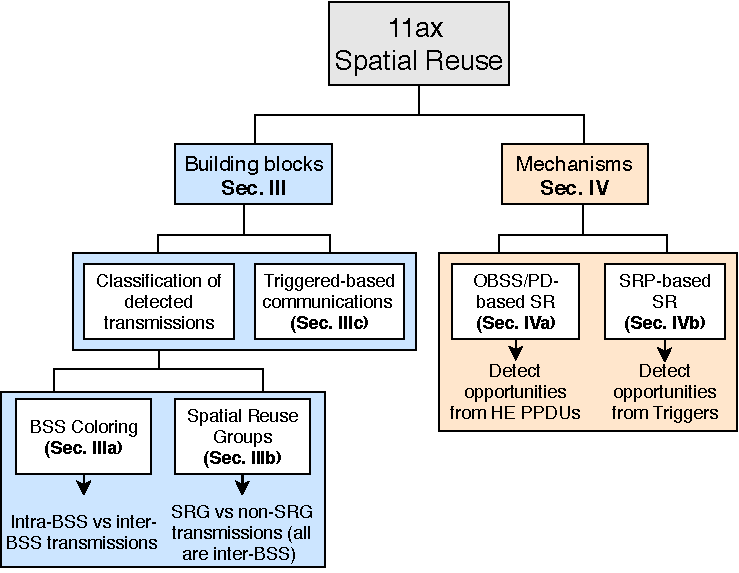
\includegraphics[width=0.7\columnwidth]{sr_summary}
	\caption{Summary of the 11ax SR operation.}
	\label{fig:sr_summary}
\end{figure}

To illustrate the potential SR enhancement in an OBSS, let us focus on Fig.~\ref{fig:spatial_reuse_11ax}. Unlike typical coverage representations in wireless networks, throughout this paper, we consider the carrier sense area of each device (instead of the generated interference). For that, our representation assumes that the transmission power used by any device is fixed and that all the BSSs use the same frequency channel, which allows focusing on the spatial interactions only. Accordingly, the dashed circles in Fig.~\ref{fig:spatial_reuse_11ax} indicate the transmitters that can be detected by the node of interest. In our example, both Access Points (APs) can simultaneously transmit to their corresponding stations (STAs), provided that they use the enhanced combination of CST and transmission power (bold line). In contrast, parallel transmissions are not possible when using the default configuration.
\begin{figure}[ht!]
	\centering
	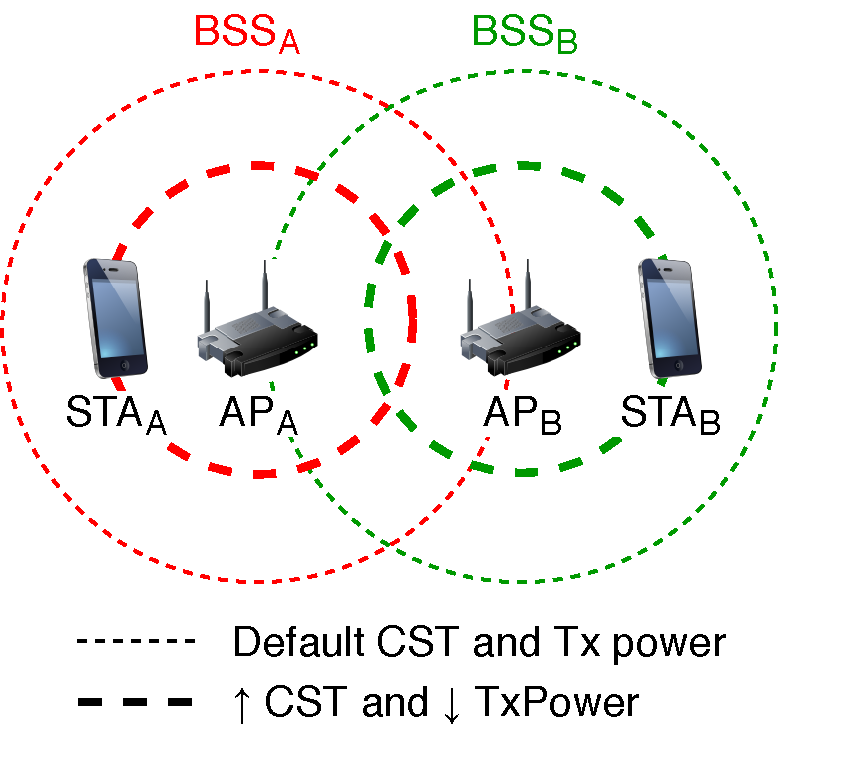
\includegraphics[width=0.5\textwidth]{fig_1.pdf}
	\caption{SR enhancement through CST adjustment and TPC. The carrier sensing area of each transmitter is graphically represented by the dashed lines.}
	\label{fig:spatial_reuse_11ax}
\end{figure}

In spite of the apparent benefits of the SR operation, its actual potential is still unknown. \textcolor{black}{The fact is that SR depends on multiple factors, such as the network topology, the type of propagation effects, or the type of radio used by devices \cite{guo2003spatial}. Moreover, sensitivity adjustment and power control may result in asymmetric links that can potentially lead to unfairness situations \cite{mhatre2007interference}.} In some cases, dynamic sensitivity and transmission power adjustment have been shown to significantly increase the network performance and to contribute to reducing the effects of the well-known hidden and exposed terminal problems \cite{zhou2005balancing}. However, in some other cases, these problems may be exacerbated \cite{wilhelmi2019potential}. Indeed, modifying either the CST or the transmit power can worsen the hidden/exposed terminal problems by generating flow starvation and asymmetries.

Figure \ref{fig:policies_sr} shows in an intuitive manner the effect of increasing and decreasing both the transmission power and the sensitivity in WLANs. For instance, increasing the sensitivity of a device may contribute to accessing the channel more often since the listening area is reduced. However, this can lead to observing a higher number of collisions by hidden-node. Moreover, using a more aggressive channel access policy may expose the receivers to a higher level of interference, thus requiring the utilization of more robust Modulation and Coding Scheme (MCS).
\begin{figure}[ht!]
	\centering
	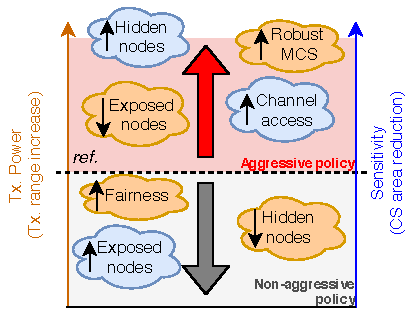
\includegraphics[width=0.5\textwidth]{policies_sr}
	\caption{Effects of different policies with regards to sensitivity adjustment and transmission power control.}
	\label{fig:policies_sr}
\end{figure}

As discussed, dealing with the spatial dimension has different kinds of implications and leads to complex inter-BSS interactions that are hard to predict beforehand. Indeed, the 11ax SR operation is one of the least studied features in next-generation WLANs and only a few works have devised its potential. Firstly, the authors in \cite{mori2014performance} evaluated the benefits of using dynamic sensitivity thresholds for inter-BSS transmissions, given a fixed transmit power. Secondly, the work in \cite{qu2018survey} exhaustively surveyed the 11ax amendment, thus providing an overview of the first drafted SR operation. Moreover, it provided some results on applying SR in both indoor and outdoor scenarios, showing a higher potential for indoor deployments. Similarly, the authors in \cite{shen2018research} introduced the contents of the 11ax SR as they are described in the amendment. In addition, they provided a performance evaluation based on the adjustment of the inter-BSS sensitivity threshold. Their results showed significant gains when applying SR, especially for dense scenarios. 

Unlike in \cite{mori2014performance, qu2018survey, shen2018research}, in this paper we delve into the 11ax SR operation in more detail since we consider the two different SR operations included in the 11ax amendment. In addition, our analysis of the 11ax SR is not limited to the technical information included in the amendment. Instead, we accompany our descriptions with illustrative use cases, thus bringing a new perspective that allows devising the real utility behind the operation. We thus go beyond the definition of the specification, shedding light on its purpose, benefits, and challenges.

% Contributions
Our aim in this paper is to provide a comprehensive tool for researchers interested in the topic and to analyze the potential of the SR operation in future WLANs. Besides, we focus on the potential gaps in the standard to be filled by the research community. The main contributions of this paper lie in the description, analysis, and evaluation of the 11ax SR operation. In particular:
\begin{enumerate}
	\item We provide a gentle, exhaustive, and comprehensive overview of the SR operation included in the 11ax amendment.
	\item We analytically model the 11ax SR operation for the sake of capturing the new kinds of inter-BSS interactions and understanding their implications. The results of this model are verified with the Komondor 11ax-based simulator \cite{barrachina2019komondor}.
	\item We study the potential performance gains of the 11ax SR operation through simulations. 
	\item We delve into the gaps and gray areas existing in the current 11ax SR operation and provide forecasts of future research directions in the field.
\end{enumerate}

% Document structure
The remainder of this document is structured as follows. Section \ref{section:previous_work_sr} surveys the related work on SR in WLANs. Section \ref{section:enablers_sr_11ax} describes the specifications and procedures to enable 11ax SR, whereas Section \ref{section:operation_sr_11ax} details the operation itself. Section~\ref{section:analytical_model} presents an analysis-based study of 11ax SR in simple scenarios, which is extended in Section~\ref{section:performance_evaluation} by simulating dense deployments. Section \ref{section:ways_forwad} identifies the gaps and research opportunities found within the 11ax SR operation and explores potential ways forward. Finally, Section~\ref{section:conclusions} provides some concluding remarks.

% ----------------------------------
% -
% 	-- Previous Work on SR --
% -
% ----------------------------------
\section{Spatial Reuse techniques in IEEE 802.11 WLANs}%\section{Related Work on Spatial Reuse in IEEE 802.11 WLANs}
\label{section:previous_work_sr}
 
The problem of dynamic sensitivity and transmission power adjustment has been previously addressed in multiple ways. On the one hand, we find centralized solutions such as the ones proposed in \cite{li2011achieving, jamil2016novel, nakahira2014centralized}, where the SR operation is controlled and mandated from the APs. Among these, we highlight \cite{jamil2016novel}, which uses a method based on Neural Networks (NN) to compute the best combination of sensitivity and transmit power to be used by all the BSSs in a given scenario. Nonetheless, centralized approaches require coordination and extra overhead, which is usually impractical.

On the other hand, SR has been addressed through a decentralized perspective in \cite{chevillat2005dynamic, tang2011improving, chau2017effective, wilhelmi2019collaborative, wilhelmi2019potential}. Most of the decentralized strategies rely on collecting feedback on several performance metrics (e.g., sensed interference, packets lost, etc.). While works such as \cite{chevillat2005dynamic, tang2011improving, chau2017effective} propose adaptive mechanisms to adjust the CST and/or the transmission power, some others like \cite{wilhelmi2019collaborative, wilhelmi2019potential} provide probabilistic approaches based on Reinforcement Learning (RL) for finding the best possible configuration.

Concerning IEEE 802.11ax WLANs, the Dynamic Sensitivity Control (DSC) scheme was proposed to be included in the standard, but it was never incorporated. The performance of DSC was evaluated in \cite{afaqui2015evaluation, afaqui2016dynamic, kulkarni2015taming}. Furthermore, the authors in \cite{selinis2016evaluation, selinis2017exploiting} combined DSC with BSS color schemes to devise further improvements in WLANs.

The current 11ax SR operation has nonetheless been studied to a lower extent. Based on the OBSS/PD-based SR operation, the work in \cite{selinis2018control} proposed a new mechanism to adjust the OBSS/PD threshold.\footnote{The OBSS/PD threshold refers to the sensitivity to be used for detected inter-BSS transmissions.} This mechanism, so-called Control OBSS/PD Sensitivity Threshold (COST), differs from DSC in terms of the information available in 11ax nodes. In this case, nodes need to be aware of changes in the neighboring BSSs. 

Unlike previous works, we focus on the IEEE 802.11ax SR operation defined in Draft v4.0 and delve into its potential through analytical modeling and a simulation tool. Moreover, we identify potential gaps and research opportunities with regard to the amendment.

% ----------------------------------
% -
% 	-- IEEE 802.11ax Preliminaries --
% -
% ----------------------------------
\section{IEEE 802.11ax Spatial Reuse Operation: Building Blocks}
\label{section:enablers_sr_11ax}
Before delving into the 11ax SR mechanisms, we first describe the enabling concepts and features. In particular, the 11ax SR operation can be understood through \textbf{BSS coloring} and \textbf{Spatial Reuse Groups (SRG)}. In addition, we introduce the \textbf{Triggered-based (TB) transmissions} upon which the PSR operation is based.

%% BSS COLORING
\subsection{BSS coloring}	
\label{section:bss_coloring}	
BSS coloring is a key enabler of the 11ax SR operation, whereby HE nodes can rapidly identify the source of a given transmission. In case that BSS coloring is adopted in an OBSS, a given device can effectively determine whether the channel is occupied by another device belonging to the same BSS (intra-BSS transmission, same color) or from a different one (inter-BSS transmission, different color). The BSS color, which is determined by the AP and is included in the preambles of Wi-Fi frames,\footnote{The \texttt{BSS color} field is included in the Physical Layer Convergence Procedure (PLCP) header. See Appendix \ref{section:frames} for further details.} is a value in the range of 1 to 63. It remains static until the AP considers to change it. When noticing a BSS color overlap (i.e., two different BSSs use the same color), a new color may be chosen by the affected APs. 

The method for selecting a new color is out of the scope of the 11ax amendment, but the advertising operation is actually defined. An HE AP may announce a new BSS color via the \texttt{BSS Color Change Announcement} element, which is carried in Beacon, Probe Response, and (Re)Association Response frames. 

% Intra-BSS and Inter-BSS frames
\subsubsection{BSS color-based channel access rules}
\label{section:bss_color_channel_access}
When detecting a transmission, an HE node can distinguish between intra and inter-BSS frames by rapidly inspecting the \texttt{BSS color} field that is carried in every HE PLCP Protocol Data Unit (PPDU).\footnote{If the \texttt{BSS color} is not announced, frames can be classified according to the \texttt{GROUP\_ID} and \texttt{PARTIAL\_AID} in VHT PPDUs, or the MAC address in the MAC header of legacy frames (i.e., predecessor amendments of the IEEE 802.11ac).} In particular, the default PD threshold (i.e., -82 dBm) is used for intra-BSS frames. So, from now onwards, we will refer to the default PD threshold simply as Clear Channel Assessment / Carrier Sense (CCA/CS). On the contrary, when inter-BSS frames are detected, more aggressive PD thresholds can be applied to increase the number of parallel transmissions. Those PD thresholds are termed \textbf{non-SRG OBSS/PD} and \textbf{SRG OBSS/PD}. The SRG OBSS/PD is used when spatial reuse groups are allowed, which is discussed in detail in Section \ref{section:srg}.

To illustrate how BSS coloring can help at enhancing SR, let us consider the scenario shown in Fig. \ref{fig:11ax_bss_coloring_a}. We consider that $\text{AP}_{A}$ is prone to suffer from flow starvation if it uses the default CCA/CS value, which entails being in the range of both $\text{AP}_B$ and $\text{AP}_C$. Note that simultaneous downlink transmissions can be held in both $\text{BSS}_B$ and $\text{BSS}_C$ because the transmitters are not in the range of each other. This may lead to flow-in-the-middle starvation in $\text{BSS}_A$. 

The flow-in-the-middle situation can be overtaken by $\text{AP}_{A}$ if using an OBSS/PD value higher than the CCA/CS for inter-BSS frames, which would allow ignoring the transmissions sensed from $\text{AP}_B$ and $\text{AP}_C$. This procedure is illustrated in Fig. \ref{fig:11ax_bss_coloring_b}, where $\text{AP}_A$ first identifies the source of a detected transmission by inspecting its headers. Then, after detecting the source of the ongoing transmissions (indicated by the color), the non-SRG OBSS/PD threshold is applied. If the OBSS/PD threshold is high enough to ignore inter-BSS transmissions, $\text{AP}_A$ can reset the PHY and continue the backoff procedure.

\begin{figure}[ht!]
	\centering
	\subfigure[Scenario]{\label{fig:11ax_bss_coloring_a}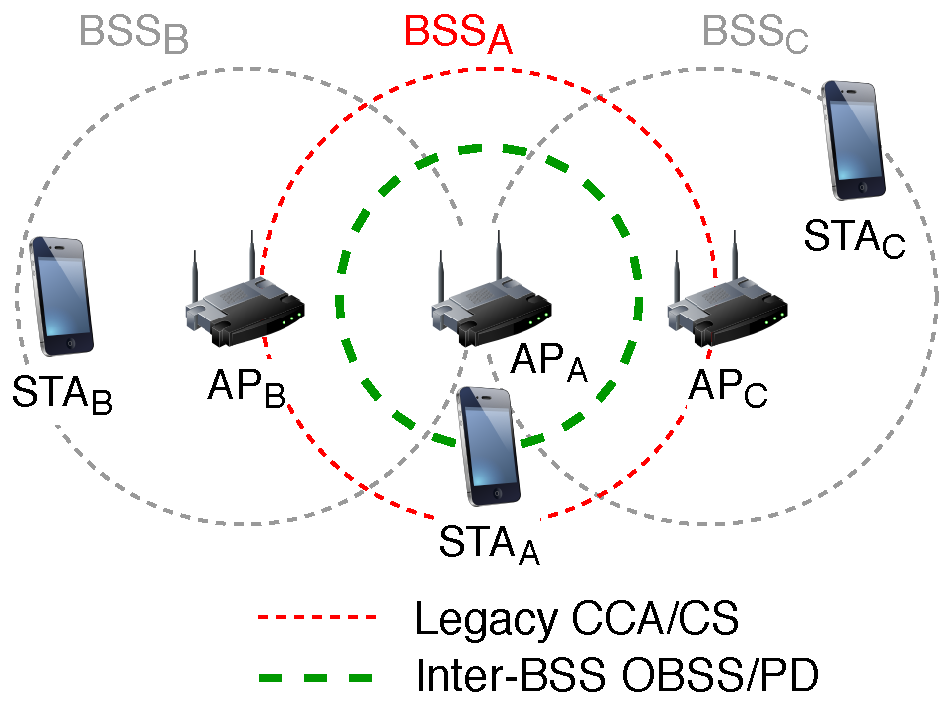
\includegraphics[width=0.45\textwidth]{fig_2a}}%
	%\hspace{1cm}%
	\subfigure[Packets exchange]{\label{fig:11ax_bss_coloring_b}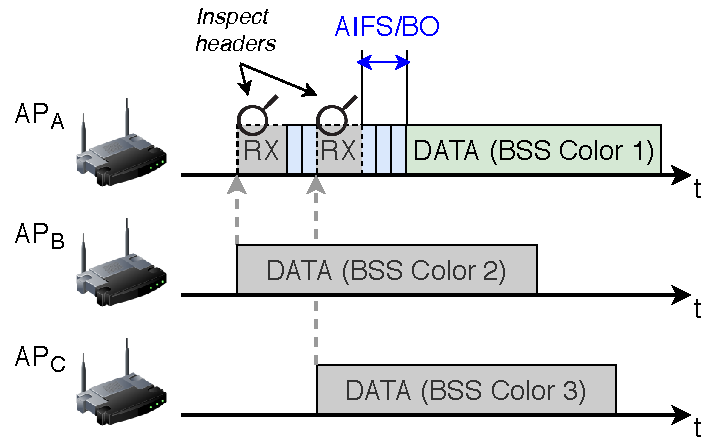
\includegraphics[width=0.5\textwidth]{fig_4b}}
	\caption{Channel access rules based on BSS coloring. In (b), the propagation delay is considered to be negligible.}
\end{figure}

% Two NAVs
\begin{figure*}[ht!]
	\centering
	\subfigure[Scenario]{\label{fig:fig_5_a}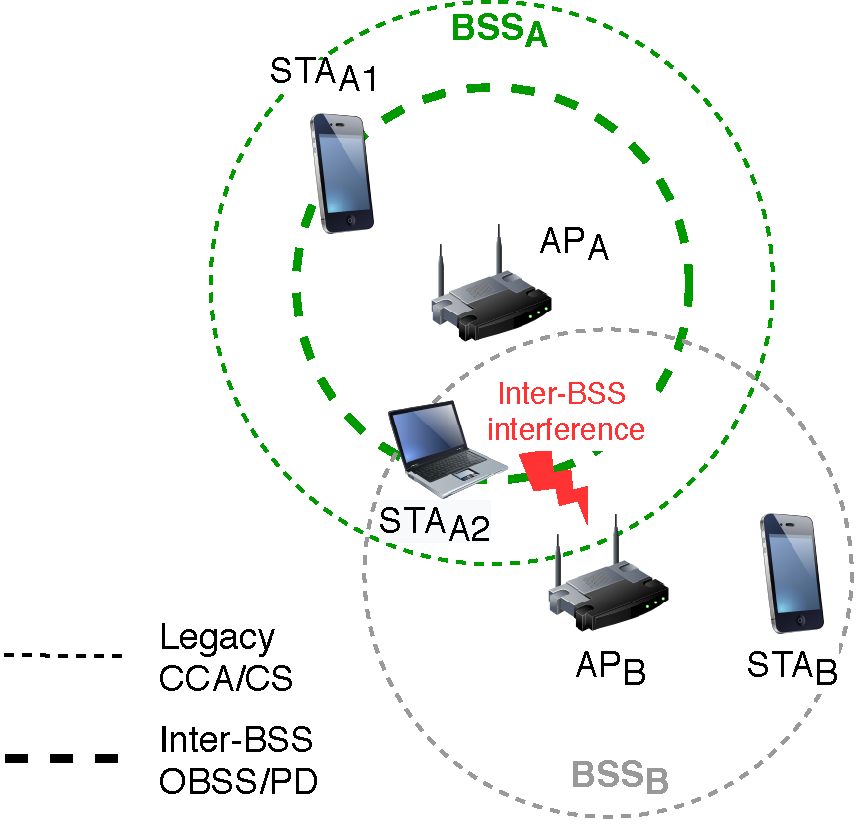
\includegraphics[width=0.4\textwidth]{fig_5_a}}
	\hspace{1cm}
	\subfigure[Packets exchange]{\label{fig:fig_5_b}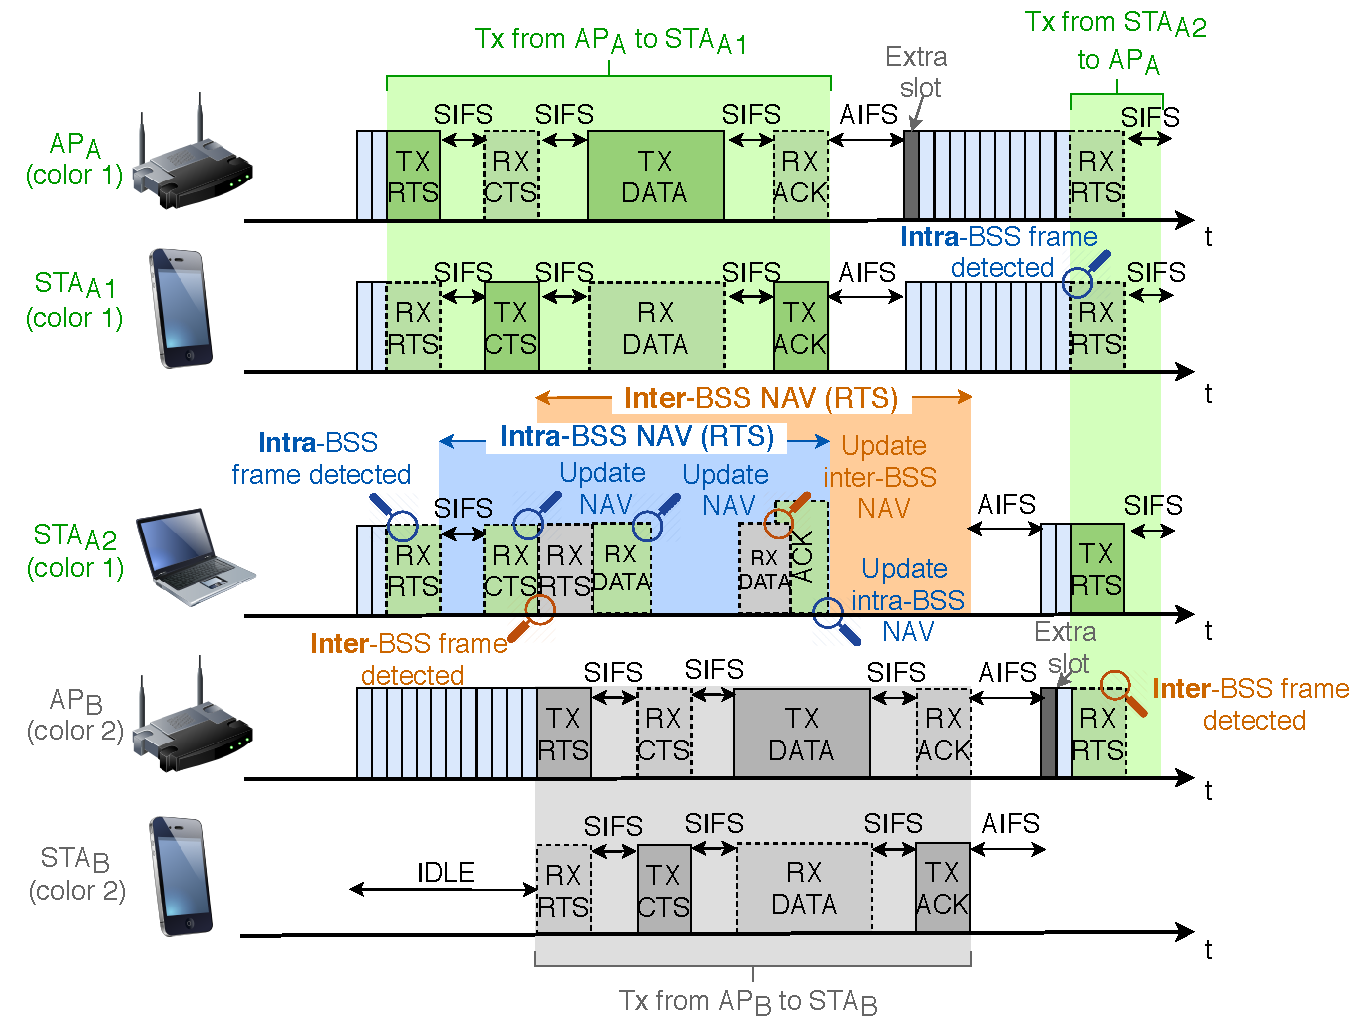
\includegraphics[width=.5\columnwidth]{fig_5_b}}
	\caption{Two NAVs operation in an OBSS.}
	\label{fig:two_navs}
\end{figure*}
\subsubsection{Two NAVs}
\label{section:two_navs}
The SR operation provides significant changes in the virtual carrier sensing procedure since two different Network Allocation Vectors (NAVs), i.e., \emph{intra-BSS NAV} and \emph{inter-BSS NAV}, have to be maintained for intra and inter-BSS frames, respectively. Accordingly, a given transmitter can decrease its backoff counter only if both NAV timers are set to zero. Otherwise, it must remain idle for at least the duration of the ongoing transmission(s),\footnote{The duration used for setting the NAV is indicated in the Duration field of RTS/CTS frames or Physical layer Service Data Units (PSDU).} which had previously activated the virtual carrier sensing. 

To showcase the utilization of two NAVs within the SR operation, we consider the scenario shown in Fig. \ref{fig:fig_5_a}, where packets are exchanged as illustrated in Fig. \ref{fig:fig_5_b}. In this scenario, $\text{BSS}_A$ and $\text{BSS}_B$ are within the same carrier sense area, provided that they both use the same CCA/CS value. In opposite, both BSSs can ignore each others' transmissions in case of using a higher OBSS/PD threshold.

Following the Distributed Coordination Function (DCF) operation, $\text{AP}_A$ initiates a downlink transmission to $\text{STA}_\text{A1}$ by first sending a Request-to-Send (RTS) frame. Then, $\text{STA}_\text{A2}$ decodes the RTS frame and realizes that it was sent by an intra-BSS device (the BSS color field matches with its own color). As a result, $\text{STA}_\text{A2}$ applies the default CCA/CS threshold to determine whether the channel remains idle or not. In this case, the sensed power is above the threshold, which makes $\text{STA}_\text{A2}$ to apply virtual carrier sensing. It is also worth mentioning that the NAV timer is confirmed in $\text{STA}_\text{A2}$ when $\text{STA}_\text{A1}$ sends the Clear-to-Send (CTS) frame to $\text{AP}_A$, because they are in the sensing range. 

In parallel to the abovementioned intra-BSS interactions, $\text{AP}_B$ starts its own downlink transmission to $\text{STA}_B$. The initiating RTS frame sent by $\text{AP}_B$ is also listened by $\text{STA}_\text{A2}$, which sets the inter-BSS NAV accordingly. On this occasion, the acknowledgments sent by $\text{STA}_B$ are ignored by $\text{STA}_\text{A2}$ due to the OBSS/PD threshold employed for inter-BSS transmissions. However, it has no impact on the modification of the inter-BSS NAV, which is properly set by the frames transmitted by $\text{AP}_B$.\footnote{Note, as well, that the amendment also allows resetting the NAV if no CTS frame is received (i.e., a timeout occurs).} After both intra and inter-BSS NAV timers are over, $\text{STA}_\text{A2}$ can perform an uplink transmission.

The utility behind maintaining two NAVs becomes evident for dense deployments. On the one hand, the intra-BSS NAV allows protecting STAs from intra-BSS transmissions, thus reducing the effect of certain anomalies such as the hidden-terminal problem. On the other hand, as a novelty, the inter-BSS NAV allows mitigating OBSS interference, which contributes to increasing the number of parallel transmissions. 

%%% SR groups
\subsection{Spatial Reuse Groups}
\label{section:srg}
To further enhance network efficiency, the 11ax amendment provides a mechanism for differentiating between two types of inter-BSS frames; that is to say, belonging or not to the same SRG. These groups can be formed by BSSs to achieve a more sophisticated SR operation. For instance, more aggressive channel access policies can be used for transmissions within the same SRG, in case that higher levels of interference could be supported by the nodes of the same SRG. Or it could be the other way around. A conservative policy can be employed for the sake of minimizing collisions by hidden nodes. 

Despite the formation of SRGs is out of the scope of the amendment, differentiating between two OBSS/PD thresholds can be useful for capturing more subtle inter-BSS interactions. Note, as well, that SRGs could be formed online to address some issues detected by an entity controlling a set of APs (e.g., belonging to the same operator).

Figure \ref{fig:fig_6} shows a deployment in which the formation of SRGs makes sense. In this case, the channel utilization can be enhanced by using the non-SRG OBSS/PD threshold to ignore inter-BSS transmissions (light dashed lines). However, using this threshold homogeneously leads $\text{STA}_C$ to suffer from packet losses. In particular, $\text{STA}_C$ cannot properly decode the information sent by $\text{AP}_C$ when $\text{AP}_A$ also occupies the channel. To solve this, $\text{BSS}_A$ and $\text{BSS}_C$ can form a group and employ a more conservative SRG OBSS/PD threshold to avoid simultaneous transmissions between the two BSSs. Notice that the non-SRG OBSS/PD threshold (which is more aggressive) can be still employed for transmissions held by any pair of BSSs involving $\text{BSS}_B$, thus increasing network efficiency. As shown, not only the formation of SRGs is a complex task, but also the definition of both non-SRG and SRG OBSS/PD thresholds.

\begin{figure}[ht!]
	\centering
	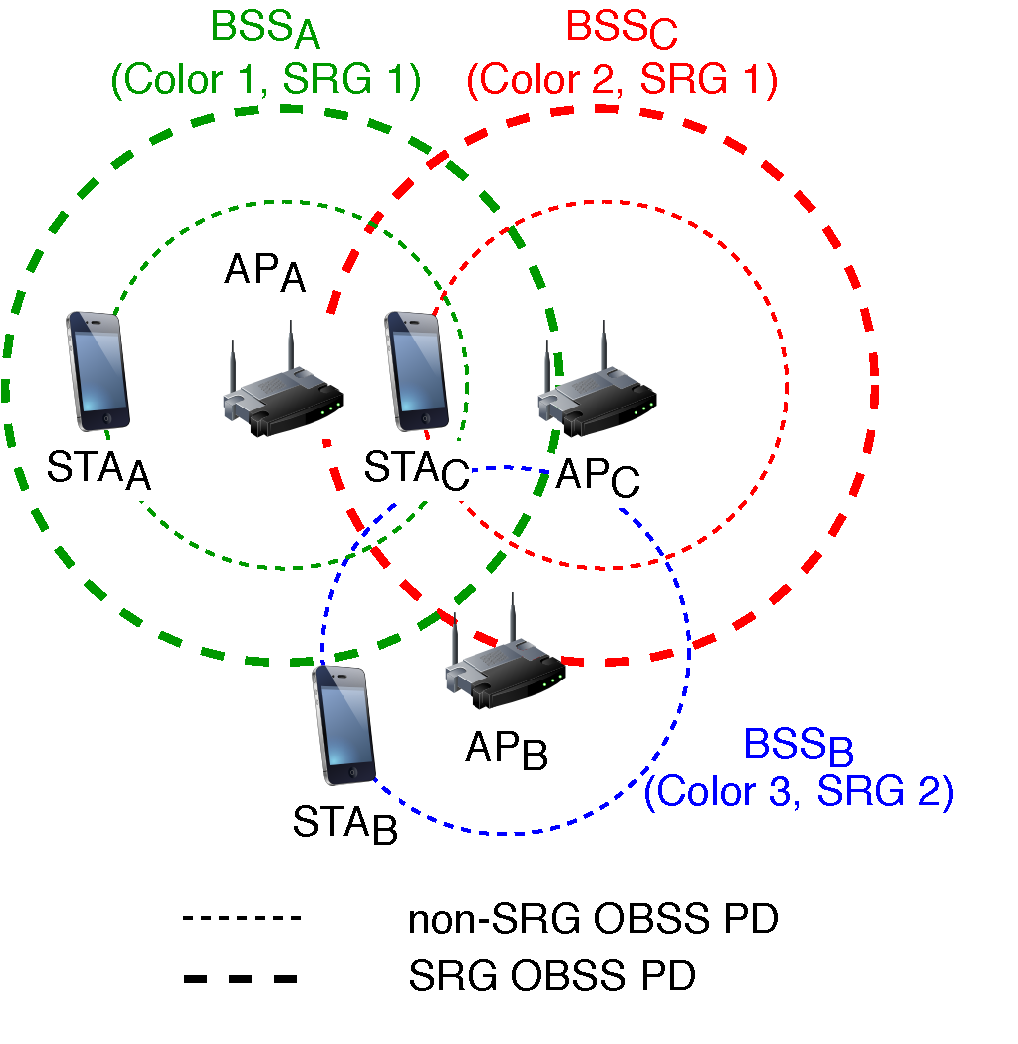
\includegraphics[width=0.5\textwidth]{fig_6}
	\caption{Spatial Reuse Groups in an OBSS.}
	\label{fig:fig_6}
\end{figure}

To apply the SR operation based on SRGs, the involved HE nodes must have indicated support for this feature. With regards to HE STAs, they enable the SRG operation upon the reception of an activating \texttt{Spatial Reuse Parameter Set} element (further described in Appendix \ref{section:srps}) from their AP. Then, for the following detected PPDUs, both HE APs and STAs may differentiate between SRG and non-SRG PPDUs. Note that 11ax devices can also identify the source of non-HE transmissions. Therefore, not only HE devices are supported but also legacy devices. The way of classifying frames according to the SRG is backward compatible with previous IEEE 802.11 amendments. Technically speaking, SRG identification is done as follows:
\begin{itemize}
	\item For HE PPDUs, an HE STA inspects the \texttt{BSS color} and checks if it belongs to the same SRG. This information is kept on the \texttt{SRG BSS Color Bitmap} of the \texttt{Spatial Reuse Parameter Set}, which stores the different BSS colors that belong to the same SRG. The AP of a given BSS is responsible for maintaining the SRG BSS Color Bitmap up to date, and to inform STAs in case of noticing any change.
	\item When it comes to VHT PPDUs, inter-BSS transmissions are considered to belong to the same SRG if the \texttt{GROUP\_ID} parameter (included in the \texttt{RXVECTOR}\footnote{The RXVECTOR constitutes a set of parameters that the PHY layer delivers to the MAC on receiving a PPDU.}) has a value of 0, and the bit in the \texttt{SRG Partial BSSID Bitmap} field corresponding to the numerical value of \texttt{PARTIAL\_AID}\footnote{The \texttt{PARTIAL\_AID} is an identifier which, similarly to the BSS color, is used by IEEE 802.11ac WLANs to quickly identify the source of a given transmission.} (also included in the \texttt{RXVECTOR}) is set to 1. 
	\item Finally, regarding other types of PPDUs, they are classified as SRG PPDUs if the BSSID information from a MAC Protocol Data Unit (MPDU) of the PPDU is correctly received and the bit in the \texttt{SRG Partial BSSID Bitmap} field corresponding to the numerical value of BSSID is 1.
\end{itemize}

% SRG and non-SRG frames
\subsubsection{SRG-based Channel Access Rules}
\label{section:srg_channel_access}
Differentiating between SRGs may provide further SR enhancements than considering only one type of inter-BSS frame. Despite the specific utilization of SRGs is also out of the scope of the 11ax amendment, we devise several situations where its application can be useful. As previously pointed out, one possibility is to establish groups for BSSs whose transmissions need to be protected. In other words, an HE STA detecting an SRG frame can implement a more conservative channel access policy. Conversely, a more aggressive policy can be applied for non-SRG PPDUs, thus increasing the number of parallel transmissions. 

To illustrate the SRG-based channel access rules, let us retake the scenario shown in Fig. \ref{fig:fig_6}, where three overlapping BSSs potentially share the medium. While $\text{BSS}_A$ and $\text{BSS}_B$ belong to SRG 1, $\text{BSS}_C$ belongs to SRG 2. Accordingly, different OBSS/PD thresholds are applied by $\text{BSS}_A$ when detecting inter-BSS frames belonging to groups 1 or 2 (note that all the BSSs use different BSS colors).

\begin{figure}[ht!]
	\centering
	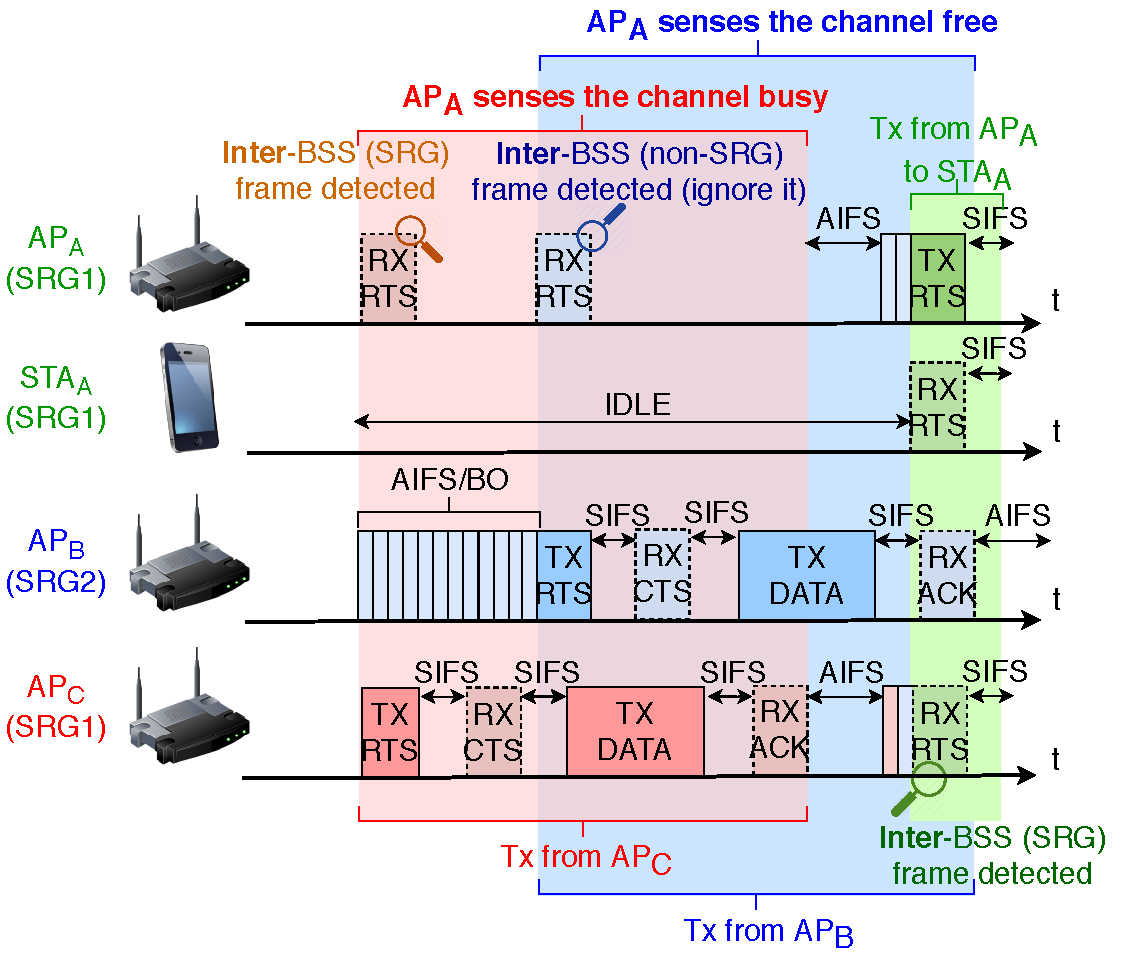
\includegraphics[width=.6\columnwidth]{fig_7}
	\caption{Packets exchange based on SRG channel access rules.}
	\label{fig:srg_channel_access}
\end{figure} 

As shown in Fig. \ref{fig:srg_channel_access}, transmissions from $\text{BSS}_C$ (in blue) provoke that $\text{AP}_A$ senses the channel busy. In contrast, packets detected from $\text{BSS}_B$ (in red) are ignored by $\text{AP}_A$ after PHY headers are properly inspected. In this example, a less restrictive OBSS/PD threshold is applied for SRG transmissions than for non-SRG ones. The fact is that $\text{STA}_B$ is sufficiently far away from $\text{AP}_A$. Therefore, simultaneous transmissions between $\text{BSS}_A$ and $\text{BSS}_B$ are completely feasible. The opposite occurs for $\text{BSS}_A$-$\text{BSS}_C$ interactions. Note that collisions may occur at STA$_C$ if simultaneous transmissions among the abovementioned BSSs are held, thus requiring additional protection.

%% TB communications
\subsection{Triggered-based communications}
\label{section:tb_communication}
As previously pointed out, one of the 11ax SR mechanisms relies on TB transmissions \cite{bellalta2019ap}. Roughly, in a TB communication, an AP schedules UL transmissions from one or more STAs. To that purpose, a Trigger Frame (TF) is sent by a given AP to indicate the group of users that are allowed to transmit during the current Transmission Opportunity (TXOP), along with other relevant information. 

Fig. \ref{fig:TB_transmission_example} illustrates an example of a TB transmission. After gaining access to the channel, the AP first sends a TF packet, which is received by HE STAs. Upon successful reception of the TF, STAs start simultaneous TB UL transmissions, which can be enabled by using multiple antenna technologies (i.e., MU-MIMO) or different OFDMA subcarriers. Once all the UL transmissions finish, the AP acknowledges all the packets with a multi-station block ACK (MACK).

\begin{figure}[ht!]
	\centering
	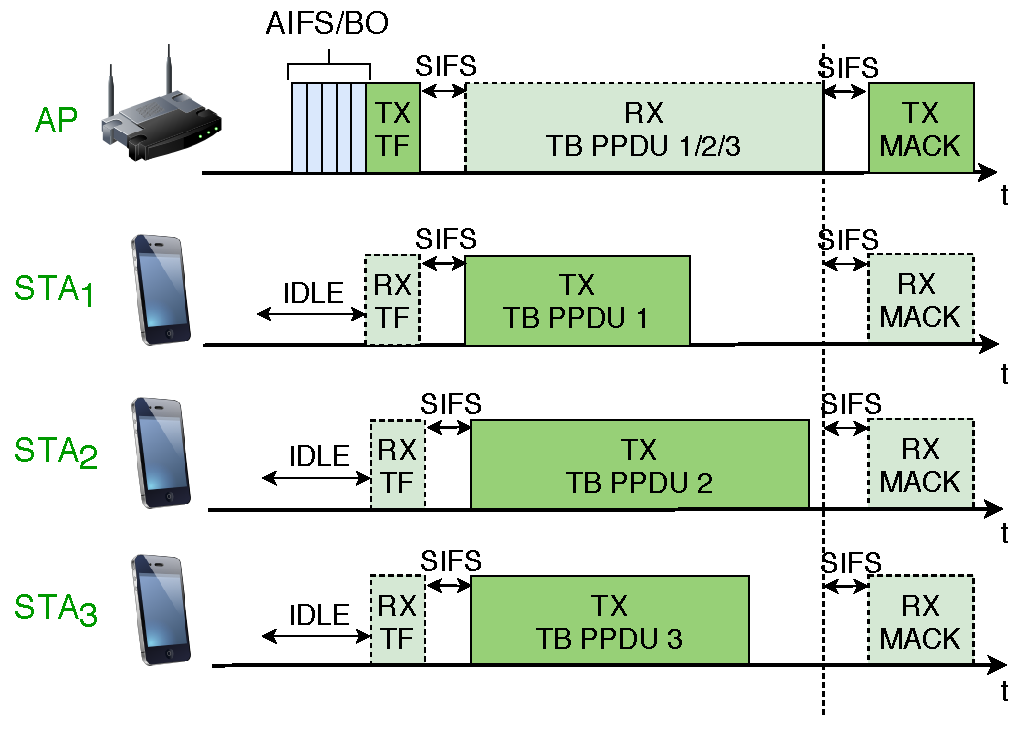
\includegraphics[width=.55\textwidth]{fig_8}
	\caption{TB UL transmission held in a BSS.}
	\label{fig:TB_transmission_example}
\end{figure}

SR in 11ax takes advantage of TB communications for detecting the so-called PSR opportunities. By inspecting an inter-BSS TF packet, an HE STA implementing PSR can determine the maximum allowed interference supported by the inter-BSS AP scheduling the transmission. As a result, it can transmit during the TXOP at a regulated transmission power. Further details on PSR are provided in Section \ref{section:srp_based}.

Finally, it is worth mentioning that, before scheduling a UL transmission, APs can cancel the virtual carrier sensing of their STAs by sending a Contention Free End (CF-End) control frame. This is done to reduce the idle periods provoked by inter-BSS transmissions, thus enhancing network efficiency. 

% ----------------------------------
% -
% 	-- IEEE 802.11ax --
% -
% ----------------------------------

\section{IEEE 802.11ax Spatial Reuse Operation}
\label{section:operation_sr_11ax}
The IEEE 802.11ax SR operation is divided into two different mechanisms: \emph{i)} \textbf{OBSS/PD-based SR} and \emph{ii)} \textbf{PSR}. So far, we have described the elements that enable both operations, thus providing insights on the potential of applying SR. In this Section, we show the technical details of IEEE 802.11ax SR, thus embodying the concepts that have been previously introduced in Section \ref{section:enablers_sr_11ax}.

%% OBSS_PD-BASED SR
\subsection{OBSS/PD-based Spatial Reuse}
\label{section:obss_pd_based}
The OBSS/PD-based SR operation is based on CST and transmit power adjustment for detected inter-BSS frames. By knowing the source of an ongoing transmission, an HE STA may employ higher CST values for the sake of improving the probability of accessing the channel. In particular, upon PPDU reception, the MAC layer of a given device receives a notification from the PHY. At that moment, the node inspects the packet and, among several operations, it determines whether the PPDU is an intra-BSS or an inter-BSS frame. The latter may be subdivided into SRG or non-SRG frames, provided that SRGs are enabled.

% General constraints
\subsubsection{General constraints}
As a general rule, the OBSS/PD threshold that is used for detected inter-BSS frames cannot exceed a certain value. This upper bound is illustrated in Fig. \ref{fig:fig_7}, and is defined as follows:
\begin{align}\nonumber \text{OBSS/PD} \leq & \max\Big(\text{OBSS/PD}_{\min}, \min\big(\text{OBSS/PD}_{\max},\\ & \text{OBSS/PD}_{\min} + (\text{TX\_PWR}_{\text{ref}}-\text{TX\_PWR})\big)\Big), \nonumber \end{align}
where $\text{OBSS/PD}_{\min}$ and $\text{OBSS/PD}_{\max}$ are set to $-82$ dBm and $-62$ dBm, respectively, the reference power $\text{TX\_PWR}_{\text{ref}}$ is set to 21 or 25 dBm, based on the
capabilities of the device,\footnote{The $\text{TX\_PWR}_{\text{ref}}$ is set to 21 dBm at HE nodes which \texttt{Highest NSS Supported M1} field is equal or less than 1. Otherwise, the  $\text{TX\_PWR}_{\text{ref}}$ is set to 25 dBm. The \texttt{Highest NSS Supported M1} subfield is part of the \texttt{Tx Rx HE MCS Support} field of the \texttt{HE Capabilities element}.} and $\text{TX\_PWR}$ is the transmission power at the antenna connector in dBm of the HE node that identifies the SR-based opportunity.
\begin{figure}[ht!]
	\centering
	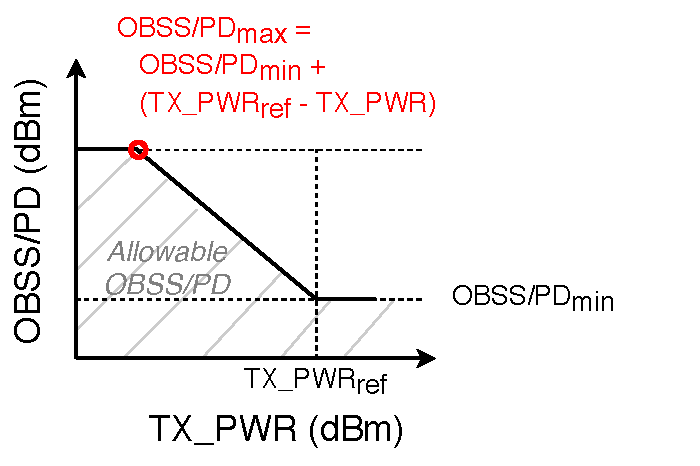
\includegraphics[width=0.6\textwidth]{fig_10}
	\caption{Graphical representation of the adjustment rules for OBSS/PD and transmission power \cite{tgax2019draft}.}
	\label{fig:fig_7}
\end{figure}

Note that the $\text{OBSS/PD}$ is defined for 20 MHz PPDUs received on the primary channel, but, in general, this value depends on the bandwidth used. In particular, the $\text{OBSS/PD}$ increases 3 dB each time the channel width is doubled, as shown in Table \ref{tbl:sensitivity_channel_width}.
\begin{table}[ht!]
	\centering
	\begin{tabular}{|c|c|}
		\hline
		\textbf{Channel width} & \textbf{OBSS/PD} \\ \hline
		40 MHz & $\text{OBSS/PD}_{20 \text{MHz}}$ + 3 dB \\ \hline
		80 MHz & $\text{OBSS/PD}_{20 \text{MHz}}$ + 6 dB \\ \hline
		160 MHz or 80+80 MHz &  $\text{OBSS/PD}_{20 \text{MHz}}$ + 9 dB \\ \hline
	\end{tabular}
	\caption{Effect of the channel width on the OBSS/PD threshold.}
	\label{tbl:sensitivity_channel_width}
\end{table}

% SRG constraints
\subsubsection{SRG-based constraints}	
In addition to the general rules for the OBSS/PD, further constraints apply when using SRGs. In particular, an AP can define certain tolerance margins for setting both the SRG and the non-SRG OBSS/PD (see Tables \ref{tbl:non-srg} and \ref{tbl:srg}). Those margins are referred to as minimum and maximum OBSS/PD offsets, respectively, and must verify:
\begin{itemize}
	\item -82 dBm $\leq$ -82 dBm + SRG OBSS/PD Min Offset dBm $\leq$ -62 dBm 
	\item SRG OBSS/PD Min Offset $\leq$ SRG OBSS/PD Max Offset
	\item SRG OBSS/PD Max Offset + -82 dBm $\leq$ -62 dBm 
	\item Non-SRG OBSS/PD Max Offset + -82 dBm $\leq$  -62 dBm
\end{itemize}

\begin{table}[ht!]
\resizebox{\columnwidth}{!}{\begin{tabular}{|c|c|c|c|}
	\hline
	\begin{tabular}[c]{@{}c@{}}\textbf{OBSS/PD SR} \\\textbf{disallowed}\end{tabular} & \textbf{Non-SRG Offset} & \begin{tabular}[c]{@{}c@{}}\textbf{Non-SRG} \\\textbf{OBSS/PD Min}\end{tabular} & \begin{tabular}[c]{@{}c@{}}\textbf{Non-SRG} \\\textbf{OBSS/PD Max}\end{tabular} \\ \hline
	Unspecified & Unspecified & -82 & -62 \\ \hline
	0 & 0 & -82 & -62 \\ \hline
	0 & 1 & -82 & \begin{tabular}[c]{@{}c@{}}-82 + Non-SRG\\ OBSS/PD Max off.\end{tabular}\\ \hline
	1 & Don't care & -82 & -82 \\ \hline
\end{tabular}}
	\caption{Minimum and maximum non-SRG OBSS/PD threshold (in dBm) to be used by a given HE STA, according to the information provided by the AP in parameters \texttt{OBSS/PD SR Disallowed} and \texttt{Non-SRG Offset Present}.}
	\label{tbl:non-srg}
\end{table}

\begin{table}[ht! ]
	\centering
	%\resizebox{\columnwidth}{!}{}
	\begin{tabular}{|c|c|c|}
			\hline
			\textbf{SRG field} & \textbf{SRG OBSS/PD Min} & \textbf{SRG OBSS/PD Max} \\ \hline	\begin{tabular}[c]{@{}c@{}}Unspecified\end{tabular} & N/A & N/A \\ \hline
			0 & N/A & N/A \\ \hline
			1 & \begin{tabular}[c]{@{}c@{}}-82 + SRG OBSS/PD\\ Min Offset\end{tabular} & \begin{tabular}[c]{@{}c@{}}-82 + SRG OBSS/PD\\ Max Offset\end{tabular} \\ \hline
	\end{tabular}
	\caption{Minimum and maximum SRG OBSS/PD values (in dBm) to be used by a given HE STA, according to the information provided by the \texttt{SRG} field. If SRG is not activated (or its value is unspecified), PPDU frames cannot be classified as SRG frames.}
	\label{tbl:srg}
\end{table}

Note, as well, that the way of computing the exact SRG and non-SRG OBSS/PD values is not defined in the standard, thus opening the door to new contributions. In relation to this, the authors of \cite{tgax2016obss_pd_evaluation} proposed using the Received Signal Strength Indicator (RSSI) of received beacons to compute it, so that $\text{OBSS/PD} =  \text{RSSI} - \text{OBSS/PD}_{\text{margin}}$. This approach is similar to the DSC procedure described in Section \ref{section:previous_work_sr}.

% Tx Power restriction
\subsubsection{Transmit power restriction}	\label{section:tx_power_restriction}
So far, we have referred to CST adjustment, but transmit power limitation is also an important part of the SR operation. In particular, a power restriction is imposed for any transmission occurring as a result of a detected SR opportunity (i.e., after ignoring a given inter-BSS frame through the OBSS/PD-based SR operation). By applying a power restriction, the standard aims to reduce the impact of these transmissions on other ongoing ones. The allowed transmit power is related to the $\text{OBSS/PD}$ employed for detecting the SR opportunity. Simply put, the more inter-BSS transmissions can be ignored (by increasing the OBSS/PD), the less interference should be generated. The transmission power restriction lasts until the end of the SR opportunity identified by an HE node, which starts when its backoff reaches zero. Notice that this period depends on the duration of the active transmission(s) used for detecting the SR opportunities. The maximum allowed transmission power ($\text{TX\_PWR}_{\max}$) is given by:
\begin{equation}
\resizebox{0.9\textwidth}{!}{%
	$\text{TX\_PWR}_{\max} = \text{TX\_PWR}_{\text{ref}} - (\text{OBSS/PD} -\text{OBSS/PD}_{\min})$}
\label{eq:power_restriction}
\end{equation}

The previous equation holds for $\text{OBSS/PD}_{\max} \geq \text{OBSS/PD} > \text{OBSS/PD}_{\min}$. Otherwise, the maximum transmission power is unconstrained.

\subsubsection{Example of OBSS/PD Spatial Reuse}
% EXAMPLES
To illustrate the OBSS/PD-based SR operation in detail, we propose the scenario shown in Fig. \ref{fig:fig_8_a}, from which we focus on $\text{STA}_\text{C2}$. In this scenario, several potential interfering devices (belonging to $\text{BSS}_A$ and $\text{BSS}_B$) surround $\text{STA}_\text{C2}$. In particular, when using the default CCA/CS, all the APs are able to transmit simultaneously. However, $\text{STA}_\text{C2}$ may suffer flow starvation because of its unprivileged location.
\begin{figure}[ht!]
	\centering
	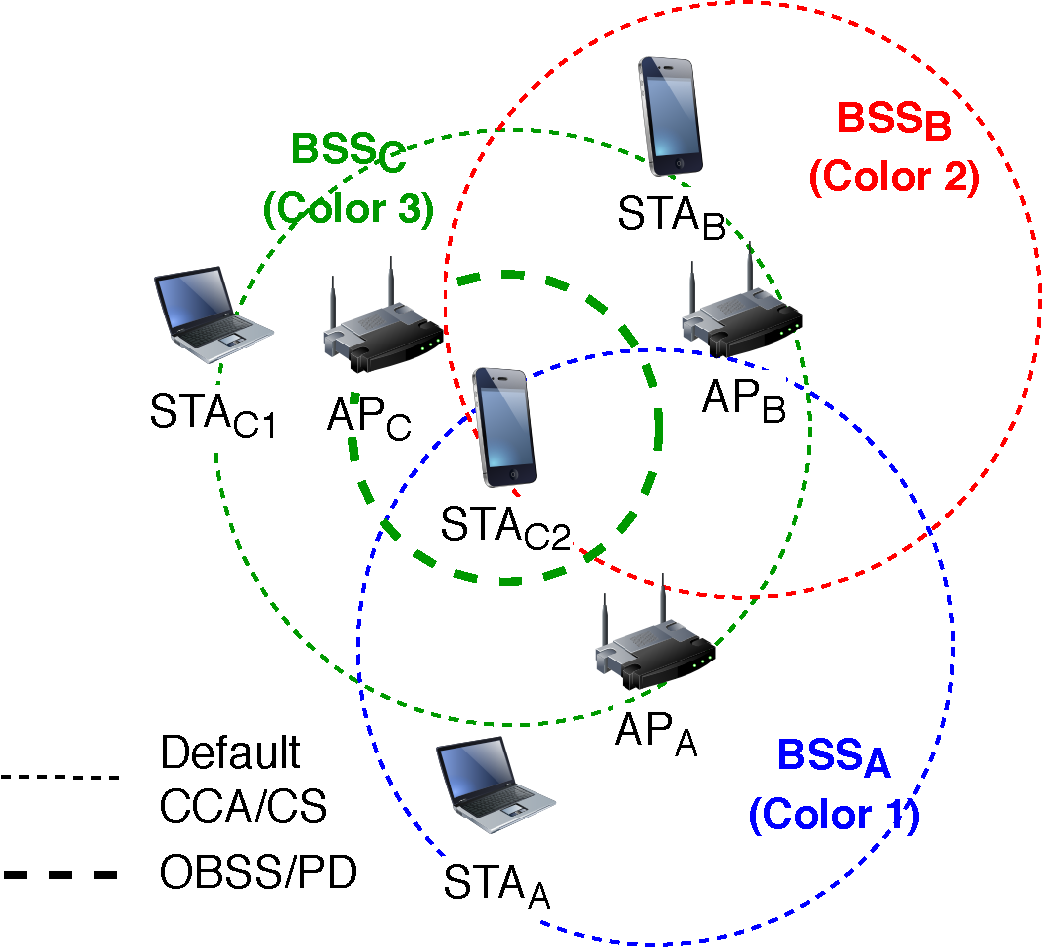
\includegraphics[width=0.55\textwidth]{fig_11}
	\caption{Scenario for showcasing the OBSS/PD SR operation.}
	\label{fig:fig_8_a}
\end{figure}

To overcome the flow starvation issue, $\text{STA}_\text{C2}$ can ignore inter-BSS transmissions, provided that the appropriate OBSS/PD value is used. Through OBSS/PD-based SR, $\text{STA}_\text{C2}$ can detect SR opportunities when nodes from $\text{BSS}_A$ and $\text{BSS}_B$ transmit. Notice that any detected SR opportunity is subject to a power restriction. Since different OBSS/PD thresholds can be maintained for different inter-BSS transmissions (of SRG and non-SRG type), different power restrictions can be used. This has to be considered before transmitting, i.e., the most restrictive power limitation should be applied when accessing the channel.

Fig. \ref{fig:fig_12} illustrates an example of packets exchange when OBSS/PD-based SR is enabled. The following particular interactions (displayed in yellow) are given:
\begin{enumerate}
	\item $\text{STA}_\text{C2}$ analyzes the RTS frame sent by $\text{AP}_A$ and classifies it as an inter-BSS frame. As a result, it applies a given OBSS/PD value that allows sensing the channel idle ($\text{RSSI}_{A \rightarrow \text{C2}} < \text{OBSS/PD}$). However, $\text{STA}_\text{C2}$ must take into account a first power restriction, which is given by Equation \eqref{eq:power_restriction}.
	\item The same procedure is followed at $\text{STA}_\text{C2}$ when detecting the RTS frame transmitted by $\text{AP}_C$. However, the transmission cannot be ignored this time because the source is an intra-BSS device (the default CCA/CS threshold is applied).
	\item As for points 1) and 2), $\text{AP}_B$'s transmission is ignored by $\text{STA}_\text{C2}$ because $\text{RSSI}_{B \rightarrow \text{C2}} < \text{OBSS/PD}$. Again, a new power restriction is considered.
	\item Finally, $\text{STA}_\text{C2}$ transmits by taking advantage of the detected SR opportunities. The transmission is nonetheless subject to a transmit power limitation, which is the more restrictive one among all the collected power restrictions (PRs). In particular, $\text{TX PWR}_{max} = \min(\text{PR}_1, \text{PR}_2)$.\footnote{Notice that, once $\text{STA}_\text{C2}$ transmits under the power restriction, the ACK sent by $\text{STA}_B$ can be ignored, so that a new power restriction is not defined.}
\end{enumerate}

\begin{figure}[ht!]
	\centering
	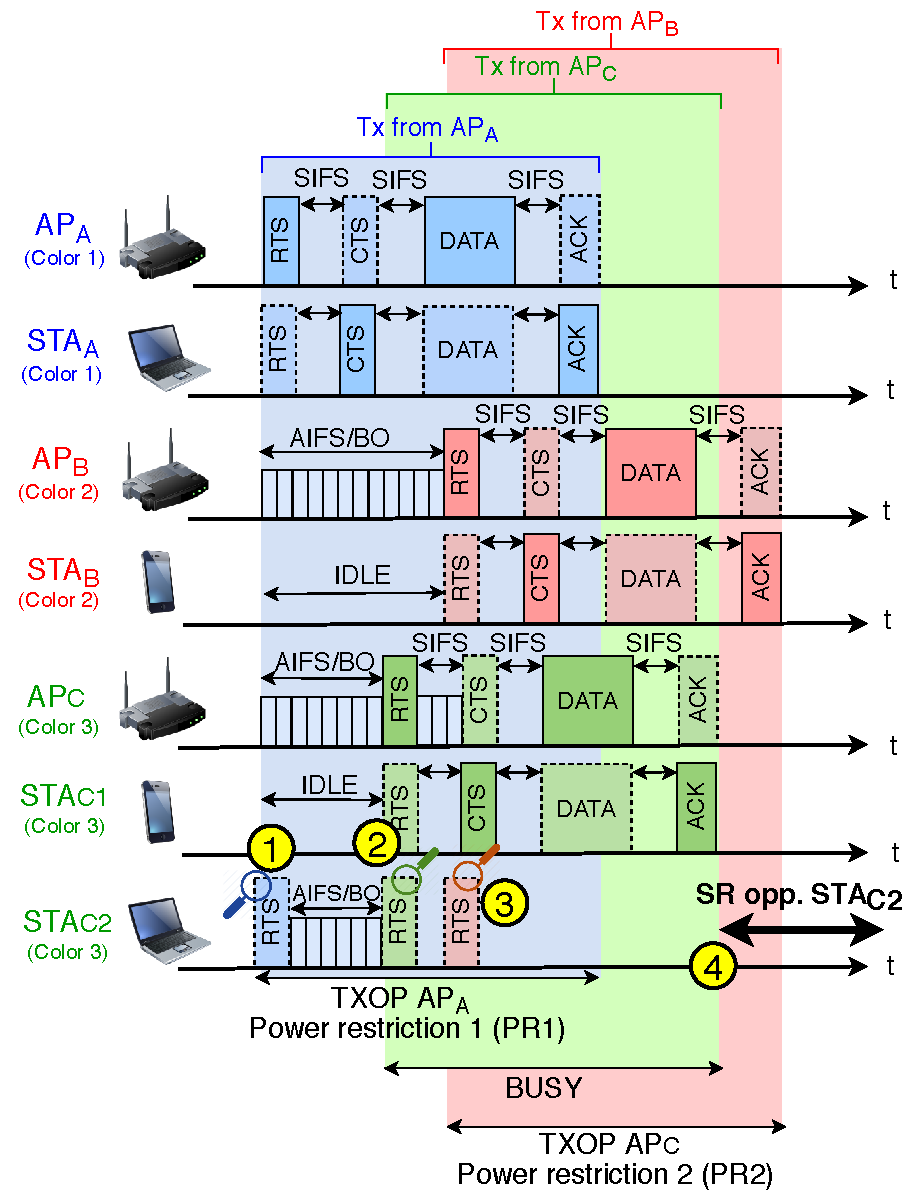
\includegraphics[width=.6\columnwidth]{fig_12}
	\caption{Example of the OBSS/PD-based SR operation. $\text{STA}_\text{C2}$ applies different OBSS/PD values according to the source of detected transmissions.}
	\label{fig:fig_12}
\end{figure}

%%% PSR
\subsection{Parametrized Spatial Reuse}
\label{section:srp_based}	
The PSR operation is based on TB transmissions and requires cooperation among the participating BSSs. On the one hand, we find nodes taking advantage of PSR opportunities (i.e., the \emph{opportunists}). These nodes identify PSR opportunities from detected TB transmissions. On the other hand, we find the \emph{transmission holders}, which perform TB transmissions and indicate support for the PSR operation. Notice that PSR opportunities can only be detected from the transmission holders that explicitly indicate support for the operation (e.g., in the headers of a TF).

When it comes to identifying PSR opportunities, an opportunist must check whether the TB PPDUs that follow a given TF packet can be ignored or not. To do so, the intended transmission power at the opportunist must not exceed the requirements imposed by the transmission holder. Those requirements are encapsulated by the latter through the \texttt{PSR\_INPUT} parameter. This parameter is indicated in the TF and can take any of the discrete values shown in Table \ref{tbl:sr_subfield_encoding_TB_ppdu}. The PSR INPUT is computed as follows:
\begin{equation}
\text{PSR INPUT} = \text{TX PWR}_\text{AP} + \text{I}_\text{AP}^{\max},
\label{eq:srp_input}
\nonumber
\end{equation}
where $\text{TX PWR}_\text{AP}$ is the normalized transmit power in dBm at the output of the antenna connector, and $\text{I}_\text{AP}^{\max}$ is a normalized value in dB that captures the maximum allowed interference at the transmission holder.\footnote{In particular, $\text{I}_\text{AP}^{\max}$ is computed as the target RSSI indicated in the TF minus the minimum SNR granting a 10\% PER (based on the highest MCS to be used for transmitting the UL HE TB PPDU). A safety margin (set by the AP) is also included not to exceed 5 dB.}

\begin{table}[ht!]
	\centering			
	\resizebox{.7\columnwidth}{!}{
		\begin{tabular}{|c|c|c|c|}
			\hline
			\textbf{Value} & \textbf{Meaning} & \textbf{Value} & \textbf{Meaning} \\ \hline
			0 & PSR\_DISALLOW & 8 & PSR = -44 dBm \\ \hline
			1 & PSR = -80 dBm & 9 & PSR = -41 dBm \\ \hline
			2 & PSR = -74 dBm & 10 & PSR = -38 dBm \\ \hline
			3 & PSR = -68 dBm & 11 & PSR = -35 dBm \\ \hline
			4 & PSR = -62 dBm & 12 & PSR = -32 dBm \\ \hline
			5 & PSR = -56 dBm & 13 & PSR = -29 dBm \\ \hline
			6 & PSR = -50 dBm & 14 & PSR $\geq$ -26 dBm \\ \hline		7 & PSR = -47 dBm & 15 & \begin{tabular}[c]{@{}c@{}}PSR\_AND\_NON-\\ SRG\_OBSS-PD\_\\ PROHIBITED\end{tabular} \\ \hline
	\end{tabular}}
	\caption{PSR subfield encoding for Trigger and HE TB PPDU frames \cite{tgax2019draft}.}
	\label{tbl:sr_subfield_encoding_TB_ppdu}
\end{table}

Once an opportunist inspects the PSR value of the detected TF\footnote{The PSR can be extracted either from the \texttt{SPATIAL REUSE} field, which is included in the \texttt{Common Info} field of the Trigger frame, or the \texttt{SIG-A PSR} field of the HE TB PPDU.} and confirms that the intended transmission power is acceptable, it transmits during the duration of the TB PPDU(s) (indicated in the \texttt{Common Info} field). In particular, the intended transmission power must be below the value of PSR minus the Received Power Level (RPL), which is measured from the legacy portion of the TF (i.e., from PHY headers).

\begin{figure}[ht!]
	\centering
	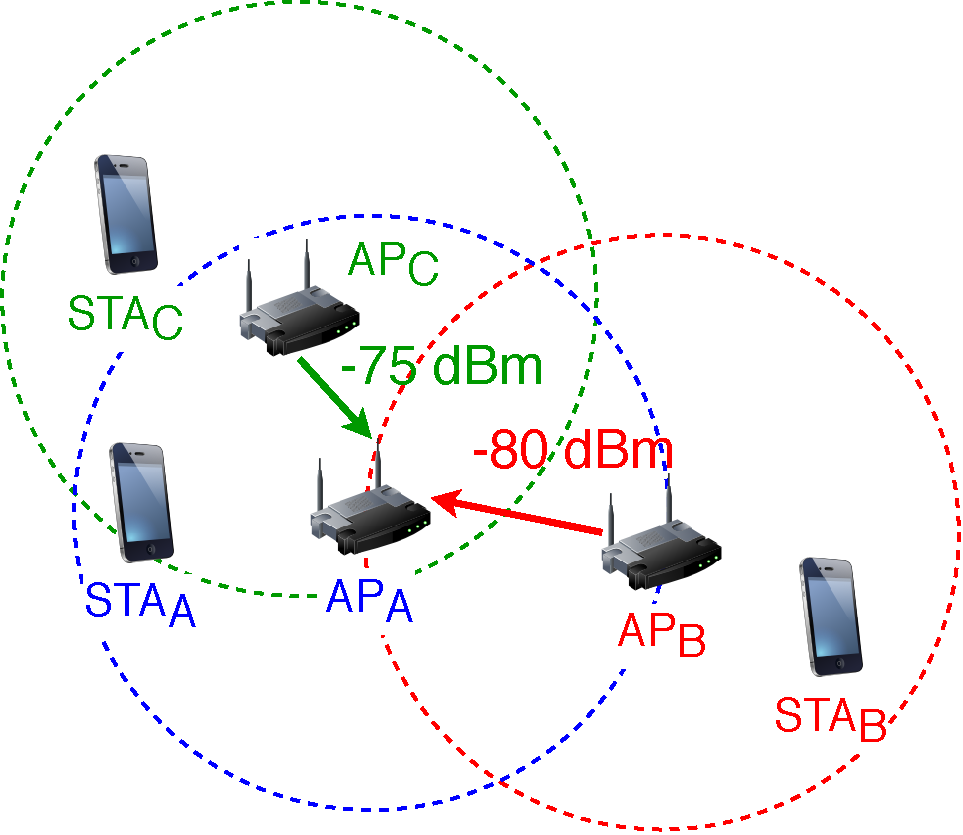
\includegraphics[width=0.5\textwidth]{fig_13a}
	\caption{Scenario for showcasing the PSR operation.}
	\label{fig:fig_13a}
\end{figure}

\begin{figure}[ht!]
	\centering
	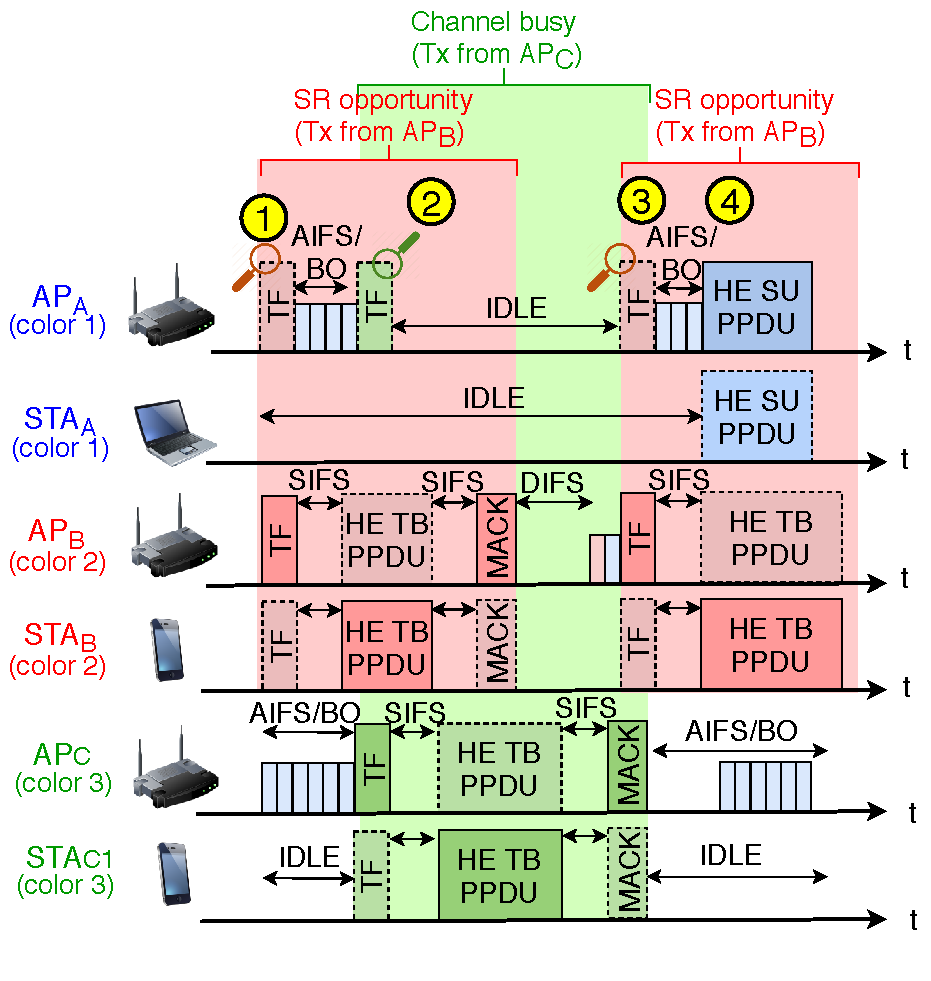
\includegraphics[width=.6\textwidth]{fig_13b}
	\caption{Packets exchange according to the PSR operation.}
	\label{fig:fig_13b}
\end{figure}

In order to illustrate the PSR operation, refer to the scenario that is shown in Fig. \ref{fig:fig_13a}, where we focus on $\text{AP}_A$. The interference sensed in that AP from the overlapping transmitters, i.e. $\text{AP}_B$ and $\text{AP}_C$, is -80 dBm and -75 dBm, respectively. According to that, Fig. \ref{fig:fig_13b} shows an example of packets exchange when applying PSR in $\text{AP}_A$. The key actions (displayed in yellow) are as follows:
\begin{enumerate}
	\item $\text{AP}_A$ detects a PSR opportunity from $\text{AP}_B$'s TF packet. Notice that the intended transmit power for the next queued packet of $\text{AP}_A$ must be lower than the indicated PSR by $\text{AP}_B$ minus the RPL. If so, $\text{AP}_A$'s backoff keeps counting down.
	\item As soon as $\text{AP}_C$ transmits a TF, the PSR opportunity previously detected by $\text{AP}_A$ is canceled because the transmit power condition no longer holds. As a result, the channel is marked as busy and the backoff countdown is frozen.
	\item For a new transmission held by $\text{AP}_B$, a PSR opportunity is detected again, even if $\text{BSS}_C$ is still transmitting. That opportunity may be used by $\text{AP}_A$ as soon as $\text{BSS}_C$'s transmission finishes.
	\item Once $\text{BSS}_C$'s transmission is over, $\text{AP}_A$ keeps the backoff countdown and transmits according to the last detected PSR opportunity.
\end{enumerate}

% ----------------------------------
% -
% 	-- Analytical Framework --
% -
% ----------------------------------
\section{Model and Simulation of the 11ax Spatial Reuse Operation}
\label{section:analytical_model}

Characterizing the IEEE 802.11ax SR operation is crucial to fully understand its implications and potential gains. However, it turns out to be a challenging task due to the complex (and still unknown) inter-BSS interactions generated by adjusting the sensitivity and the transmission power. To the best of our knowledge, none of the previous works have attempted to model the 11ax SR operation. \textcolor{black}{Nevertheless, we find other works that analyze the impact of sensitivity adjustment and transmit power control in wireless networks. In this regard, we find SINR-based methods \cite{gupta2000capacity, guo2003spatial}, which allow characterizing radio links. However, these methods typically consider the worst-case interference (i.e., nodes are assumed to transmit permanently). This entails neglecting spectrum access coordination and hence losing insights on the MAC operation.}

\textcolor{black}{Another field that is attracting a lot of attention is Stochastic Geometry (SG), which models the random nature of dense wireless networks. In particular, SG allows defining a random set of nodes (typically, based on random point processes) and deriving statistical properties on them. In telecommunications, stochastic geometry has been widely applied to model the behavior of users and to estimate metrics such as the outage probability or the throughput per area \cite{elsawy2016modeling}. Concerning SR, the works in \cite{zhao2016stochastic, zhang2015stochastic, iwata2019stochastic} apply SG to model the effect of tuning the sensitivity threshold in WLANs. However, SG models are mainly focused on PHY layer effects and fail to capture the asymmetries that may take place on applying the SR operation.}

\textcolor{black}{To address the limitations posed by the abovementioned models, we propose characterizing SR through Continuous Time Markov Networks (CTMNs) \cite{bellalta2014throughput, bellalta2017throughput}, which allow capturing both the PHY and MAC layers on estimating the throughput of a CSMA/CA network.} The analytical model presented in this work aims to provide further insight into the effects of applying SR in next-generation BSSs.

Apart from the analytical model, we introduce the 11ax SR operation in the Komondor simulator \cite{barrachina2019komondor}.\footnote{The implementation of SR can be found in Komondor v3.0, available in \url{https://github.com/wn-upf/Komondor/releases/tag/v3.0}.} The Komondor simulator was conceived, among other purposes, to allow the low-cost integration of novel mechanisms included in new IEEE 802.11 standards. This is the case of 11ax SR, which has not been yet fully implemented in any other well-known simulator. At the time of publishing this article, SR is still being developed for ns-3.\footnote{It is planned to be included in the following repository: \url{https://gitlab.com/nsnam/ns-3-dev}.} By comparing our simulation results with the analytical model, we expect to shed some light on the effects of using 11ax SR, particularly with regard to inter-BSS interactions. \textcolor{black}{The simulation of SR allows addressing the assumptions done by the CTMNs model and extend the provided results in more realistic dense environments.}

Before getting into the analysis of 11ax SR through CTMNs, it is important to mention that we have focused on the OBSS/PD-based operation described in Section \ref{section:obss_pd_based}, which has drawn much more attention than PSR. Therefore, from now onwards, we may refer to the OBSS/PD-based SR operation simply as SR. The implementation and modeling of PSR is left as future work.

\subsection{Introduction to Continuous Time Markov Networks}
The CTMN model captures the CSMA/CA operation used in IEEE 802.11 WLANs through states, which represent the set of potentially overlapping BSSs that are active at a given moment. Transitions between states occur when BSSs become active (i.e., they gain access to the medium) or when they abandon the channel (i.e., their transmission is finished). It is worth pointing out some assumptions made by the CTMN model. \textcolor{black}{First, downlink traffic is considered and the interference produced in uplink transmissions (e.g., ACKs) is not considered. Second, the backoff procedure for accessing the medium is continuous in time. Thus, collisions due to backoff expiring at the same instant are not captured by the model. Despite those are unrealistic assumptions, the model is particularly useful to depict inter-AP interactions.}

\begin{figure}[h!!!!]	
	\centering
	
\includegraphics[width=0.25\textwidth]{ctmn}
	\caption{CTMN of $\text{BSS}_A$.} 
	\label{fig:ctmn}
\end{figure}

\begin{figure*}[h!]
	\centering
	% Situation 1
	\subfigure[Sensing area (OBSS/PD = -82 dBm)]{\label{fig:cs_toy_scenario_1a}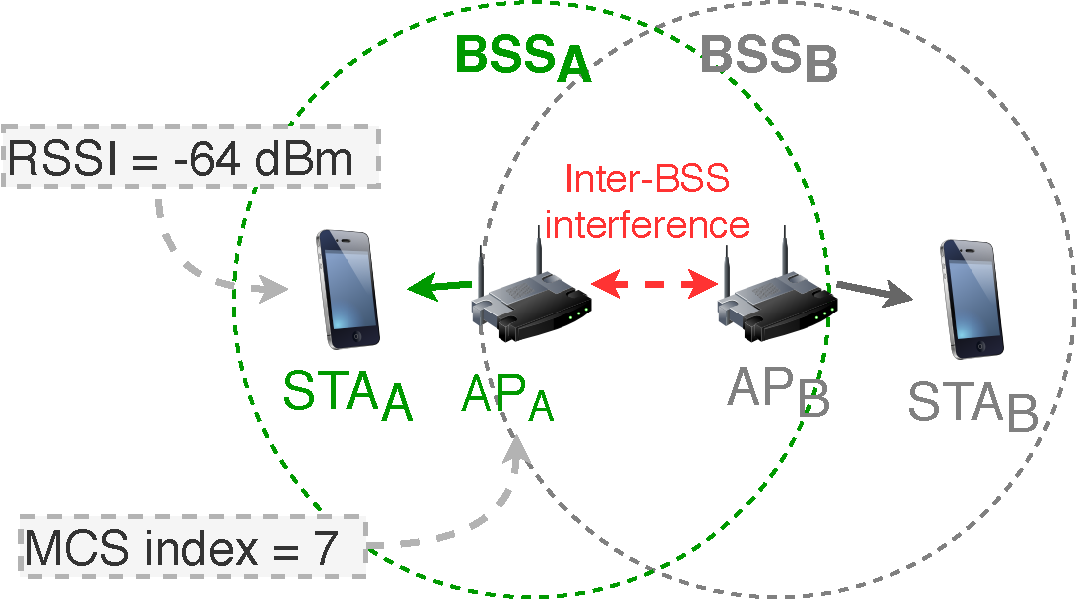
\includegraphics[width=0.4\textwidth]{fig_15a}}
	\hspace{1cm}
	% CTMN 1
	\subfigure[CTMN (OBSS/PD = -82 dBm)]{\label{fig:ctmn_toy_scenario_1a}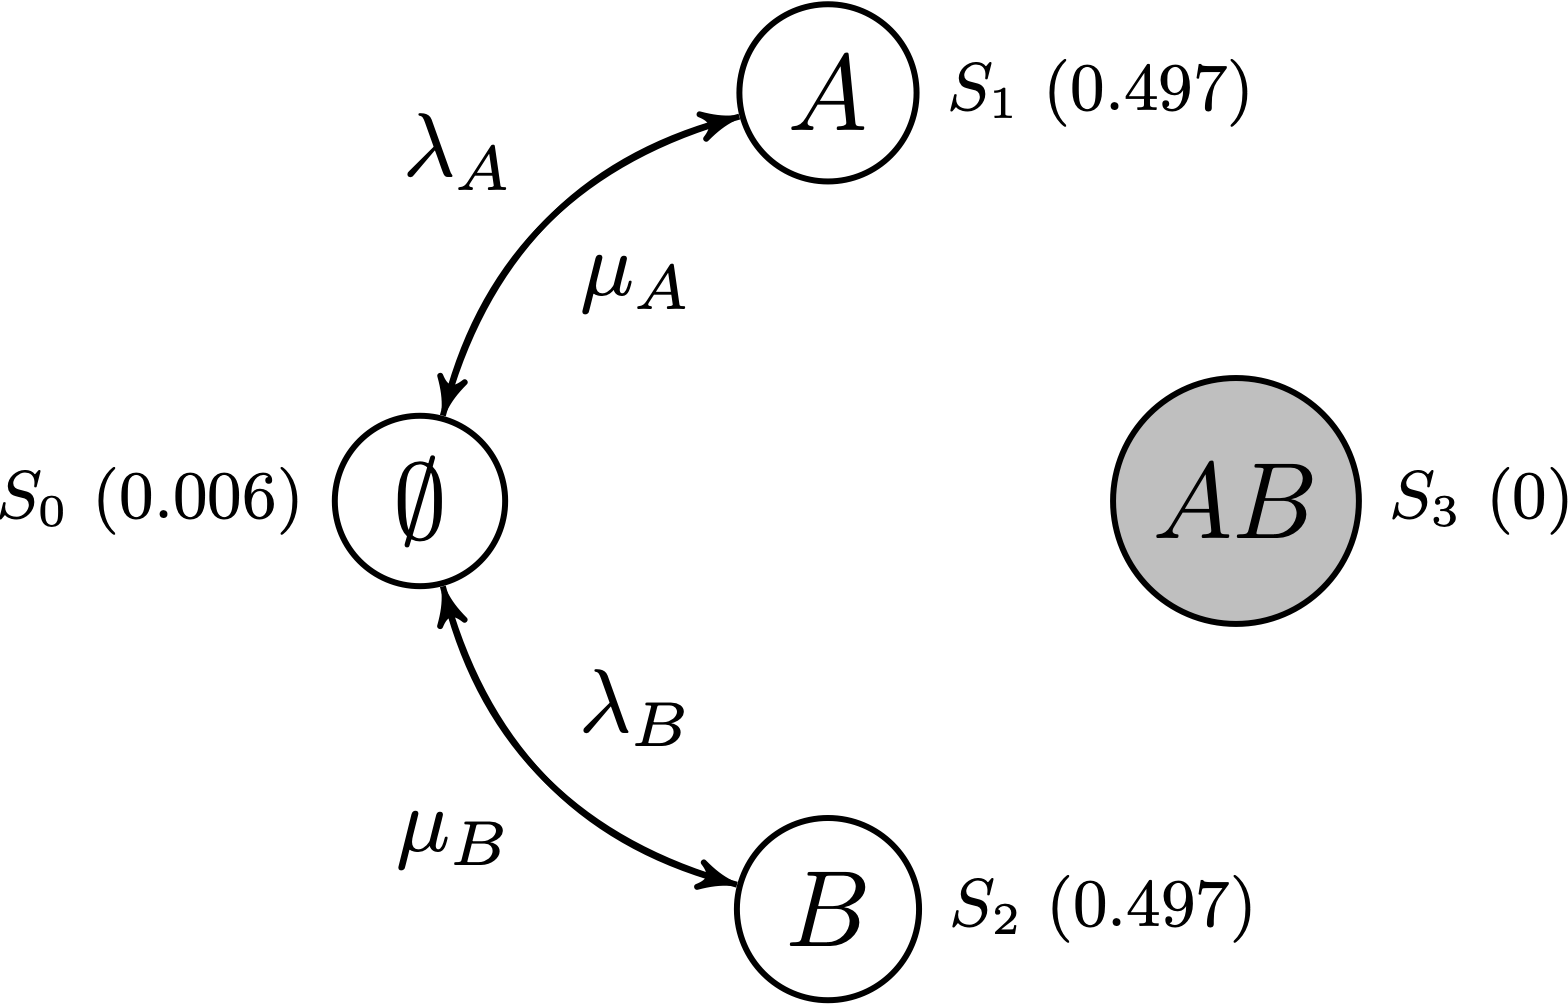
\includegraphics[width=0.4\textwidth]{ctmn_toy_scenario_1a}}\\
	% Situation 2
	\subfigure[Sensing area (OBSS/PD = -78 dBm)]{\label{fig:cs_toy_scenario_1b}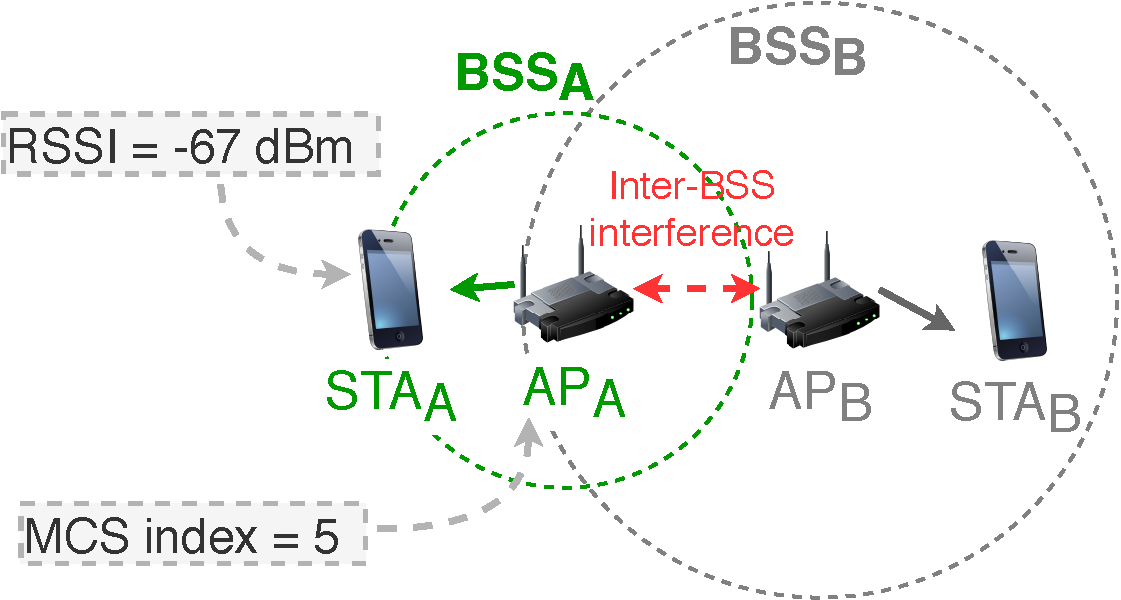
\includegraphics[width=0.4\textwidth]{fig_15c}}
	\hspace{1cm}
	% CTMN 2
	\subfigure[CTMN (OBSS/PD = -78 dBm)]{\label{fig:ctmn_toy_scenario_1b}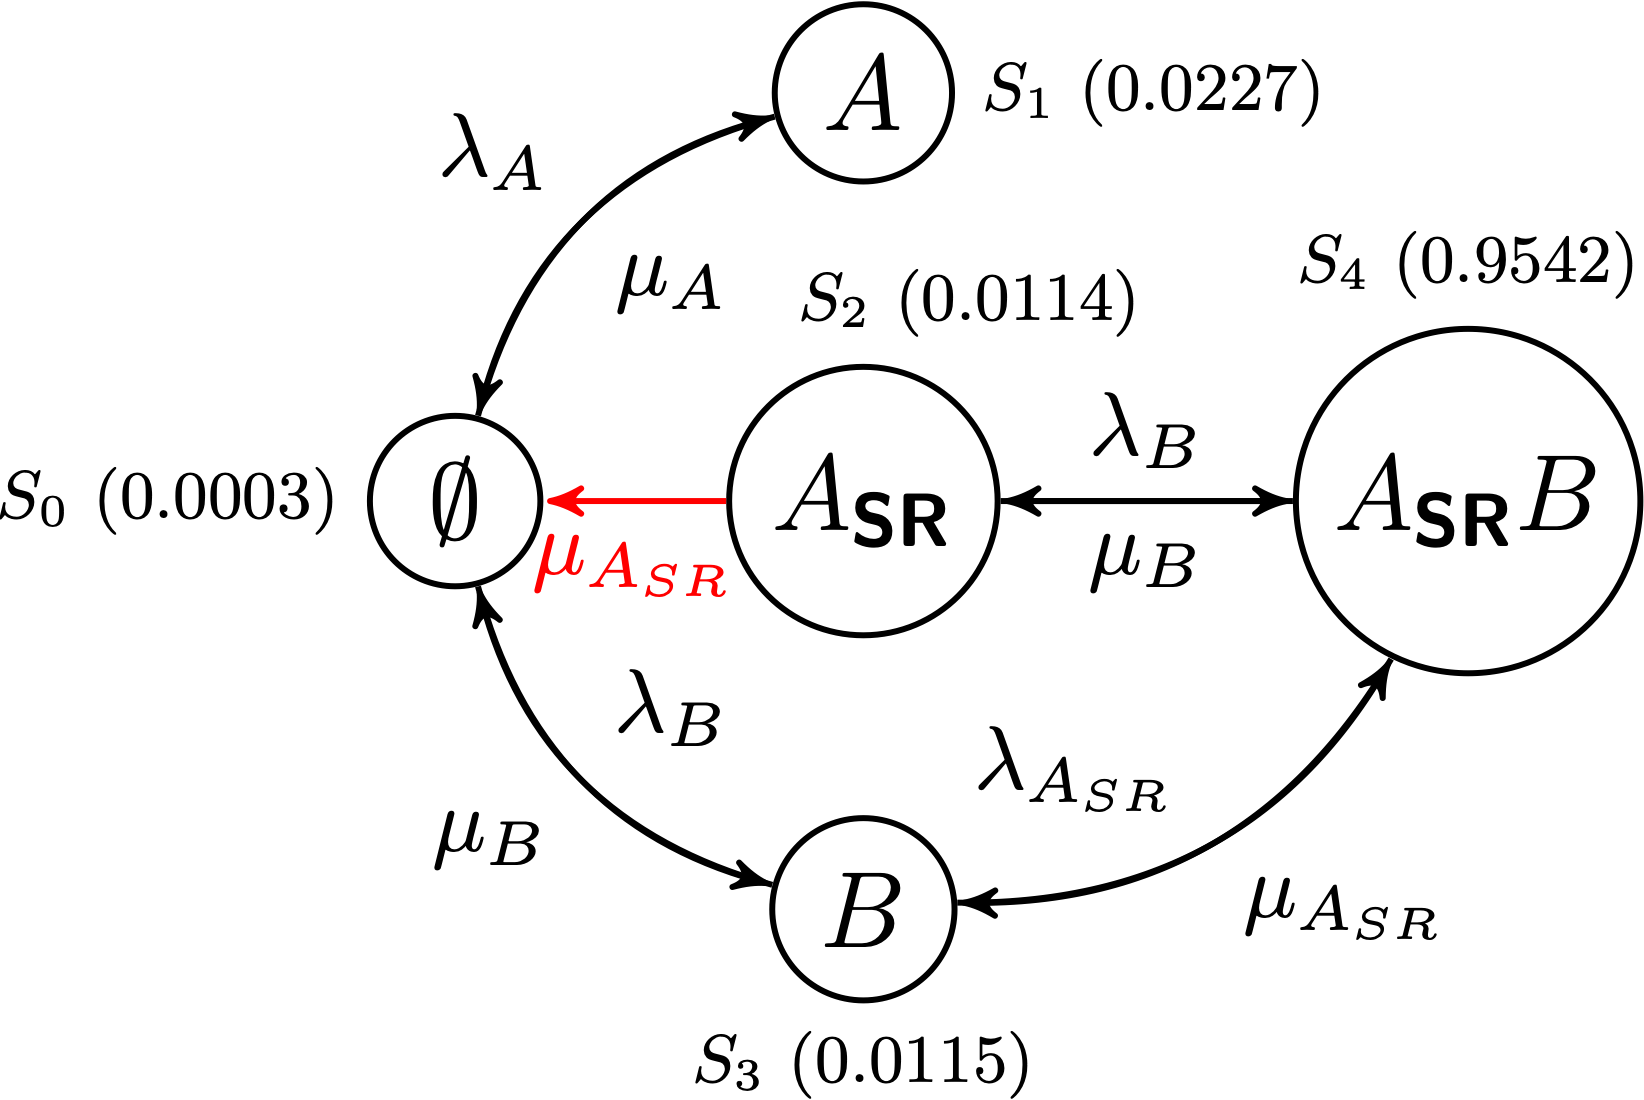
\includegraphics[width=0.4\textwidth]{ctmn_toy_scenario_1b}}%\\
	\caption{Representation of \emph{Toy scenario 1} for different settings. (a) and (c) illustrate the inter-BSS sensing area of each transmitter for OBSS/PD equal to -82 dBm and -78 dBm, respectively, whereas (b) and (d) illustrate the corresponding inter-BSS interactions through CTMNs (unidirectional transitions are shown in red).}
	\label{fig:toy_scenario_1b}
\end{figure*}

For the sake of illustration, let us consider Fig. \ref{fig:ctmn}, which represents the CTMN of a single BSS, namely $\text{BSS}_A$. In the CTMN, $s_0$ is the empty state (the channel is idle) and $s_1$ indicates that $\text{BSS}_A$ is transmitting in a given channel. Regarding the transition rates between states, we find two different types: \emph{i)} AP activates, and \emph{ii)} AP finishes a transmission. While \emph{i)} is related to the necessary time for a given node to access the channel (characterized by the arrival rate $\lambda$), \emph{ii)} depends on the time spent by a given node for transmitting data (characterized by the service rate $\mu$). Based on the transition probabilities, one can obtain the probability of every state, which allows computing the long-term throughput experienced by the different BSSs.

In this work, the 11ax SR operation has been implemented as part of the Spatial Flexible Continuous Time Markov Network (SFCTMN) framework \cite{barrachina2019dynamic, barrachina2019overlap, wilhelmi2019potential}.\footnote{A dedicated Github branch of SFCTMN has been provided for single-channel spatial reuse \cite{wilhelmi2019sfctm_spatial_reuse}.} This framework allows generating the CTMN of a given WLAN deployment, based on the spatial distribution of nodes and their configuration (e.g., range of channels used, transmission power, sensitivity, etc.). It is important to remark that additive interference is considered, which results from the combination of different simultaneous interfering transmissions. Accordingly, we are able to characterize real deployments where spatially-distributed interactions occur. Moreover, traffic is considered to be saturated in all the nodes, so that pure SR-based interactions become more apparent.

Concerning the 11ax SR operation, we have considered new states to represent the different sensitivity levels that each BSS can use based on the type of ongoing transmissions. Furthermore, the maximum allowed transmission power depends on the selected OBSS/PD threshold, which is also captured in the new SR states. Accordingly, the varying transmission capabilities of a given node (which depend on the MCS used) are represented.

%%% Simple OBSS/PD-based interactions
\subsection{Simple inter-BSS interactions}
\label{section:simple_interactions}
Through our proposed SR model, we start depicting the inter-BSS interactions that occur between two BSSs. With this aim, we introduce \emph{Toy scenario 1}, in which only $\text{BSS}_A$ implements SR. Fig. \ref{fig:cs_toy_scenario_1a} and Fig. \ref{fig:cs_toy_scenario_1b} illustrate the carrier sense areas that result from the default and the SR settings, respectively. The CTMNs capturing the inter-BSS interactions taking place in each setting are shown in Fig. \ref{fig:ctmn_toy_scenario_1a} and Fig. \ref{fig:ctmn_toy_scenario_1b}, respectively. Notice that the long-term probability of each state is shown in parentheses.

As shown in Fig. \ref{fig:cs_toy_scenario_1a} (CCA/CS is applied by both BSSs), $\text{AP}_A$ and $\text{AP}_B$ are in the carrier sense range of each other, so that parallel transmissions are not possible. This can also be noticed in the CTMN representation (see Fig. \ref{fig:ctmn_toy_scenario_1a}), where state $s_3$ (AB) cannot be reached from any other state. Nevertheless, both APs can transmit at a high rate because the maximum transmission power is used when accessing the medium. In particular, the STA in $\text{BSS}_A$ observes an RSSI of -64 dBm, which allows $\text{AP}_A$ using the MCS 7 for 20 MHz transmissions.

When it comes to the SR setting, it is possible to have simultaneous transmissions, provided that $\text{BSS}_A$ uses an OBSS/PD value greater or equal than -79 dBm. As shown in Fig. \ref{fig:cs_toy_scenario_1b}, $\text{AP}_A$ reduces its sensitivity area in case of detecting any transmission from $\text{BSS}_B$. However, ignoring inter-BSS transmissions entails a transmit power limitation. This results in poorer signal strength at the STA (RSSI = -67 dBm when the transmit power used by AP$_A$ is 17 dBm), thus forcing to use a lower data rate. The SR operation is represented through the CTMN's model in Fig. \ref{fig:ctmn_toy_scenario_1b}, where new states appear (i.e. $s_2$ and $s_4$). These new states capture the situations in which the transmitter of $\text{BSS}_A$ uses a higher OBSS/PD to ignore $\text{BSS}_B$'s transmissions (mode $A_\text{SR}$ is used, instead of $A$). In particular, state $s_2$ ($A_\text{SR}$) can never be reached from the empty state since $\text{BSS}_A$ is always expected to transmit under its default operation when the channel is idle.

The throughput achieved by $\text{BSS}_A$ and $\text{BSS}_B$ is shown Fig. \ref{fig:toy_scenario_1_results} (left side), for each possible OBSS/PD value. The transmit power limitation that is imposed on each BSS is also illustrated (right side).  
\begin{figure}[ht!]
	\centering
	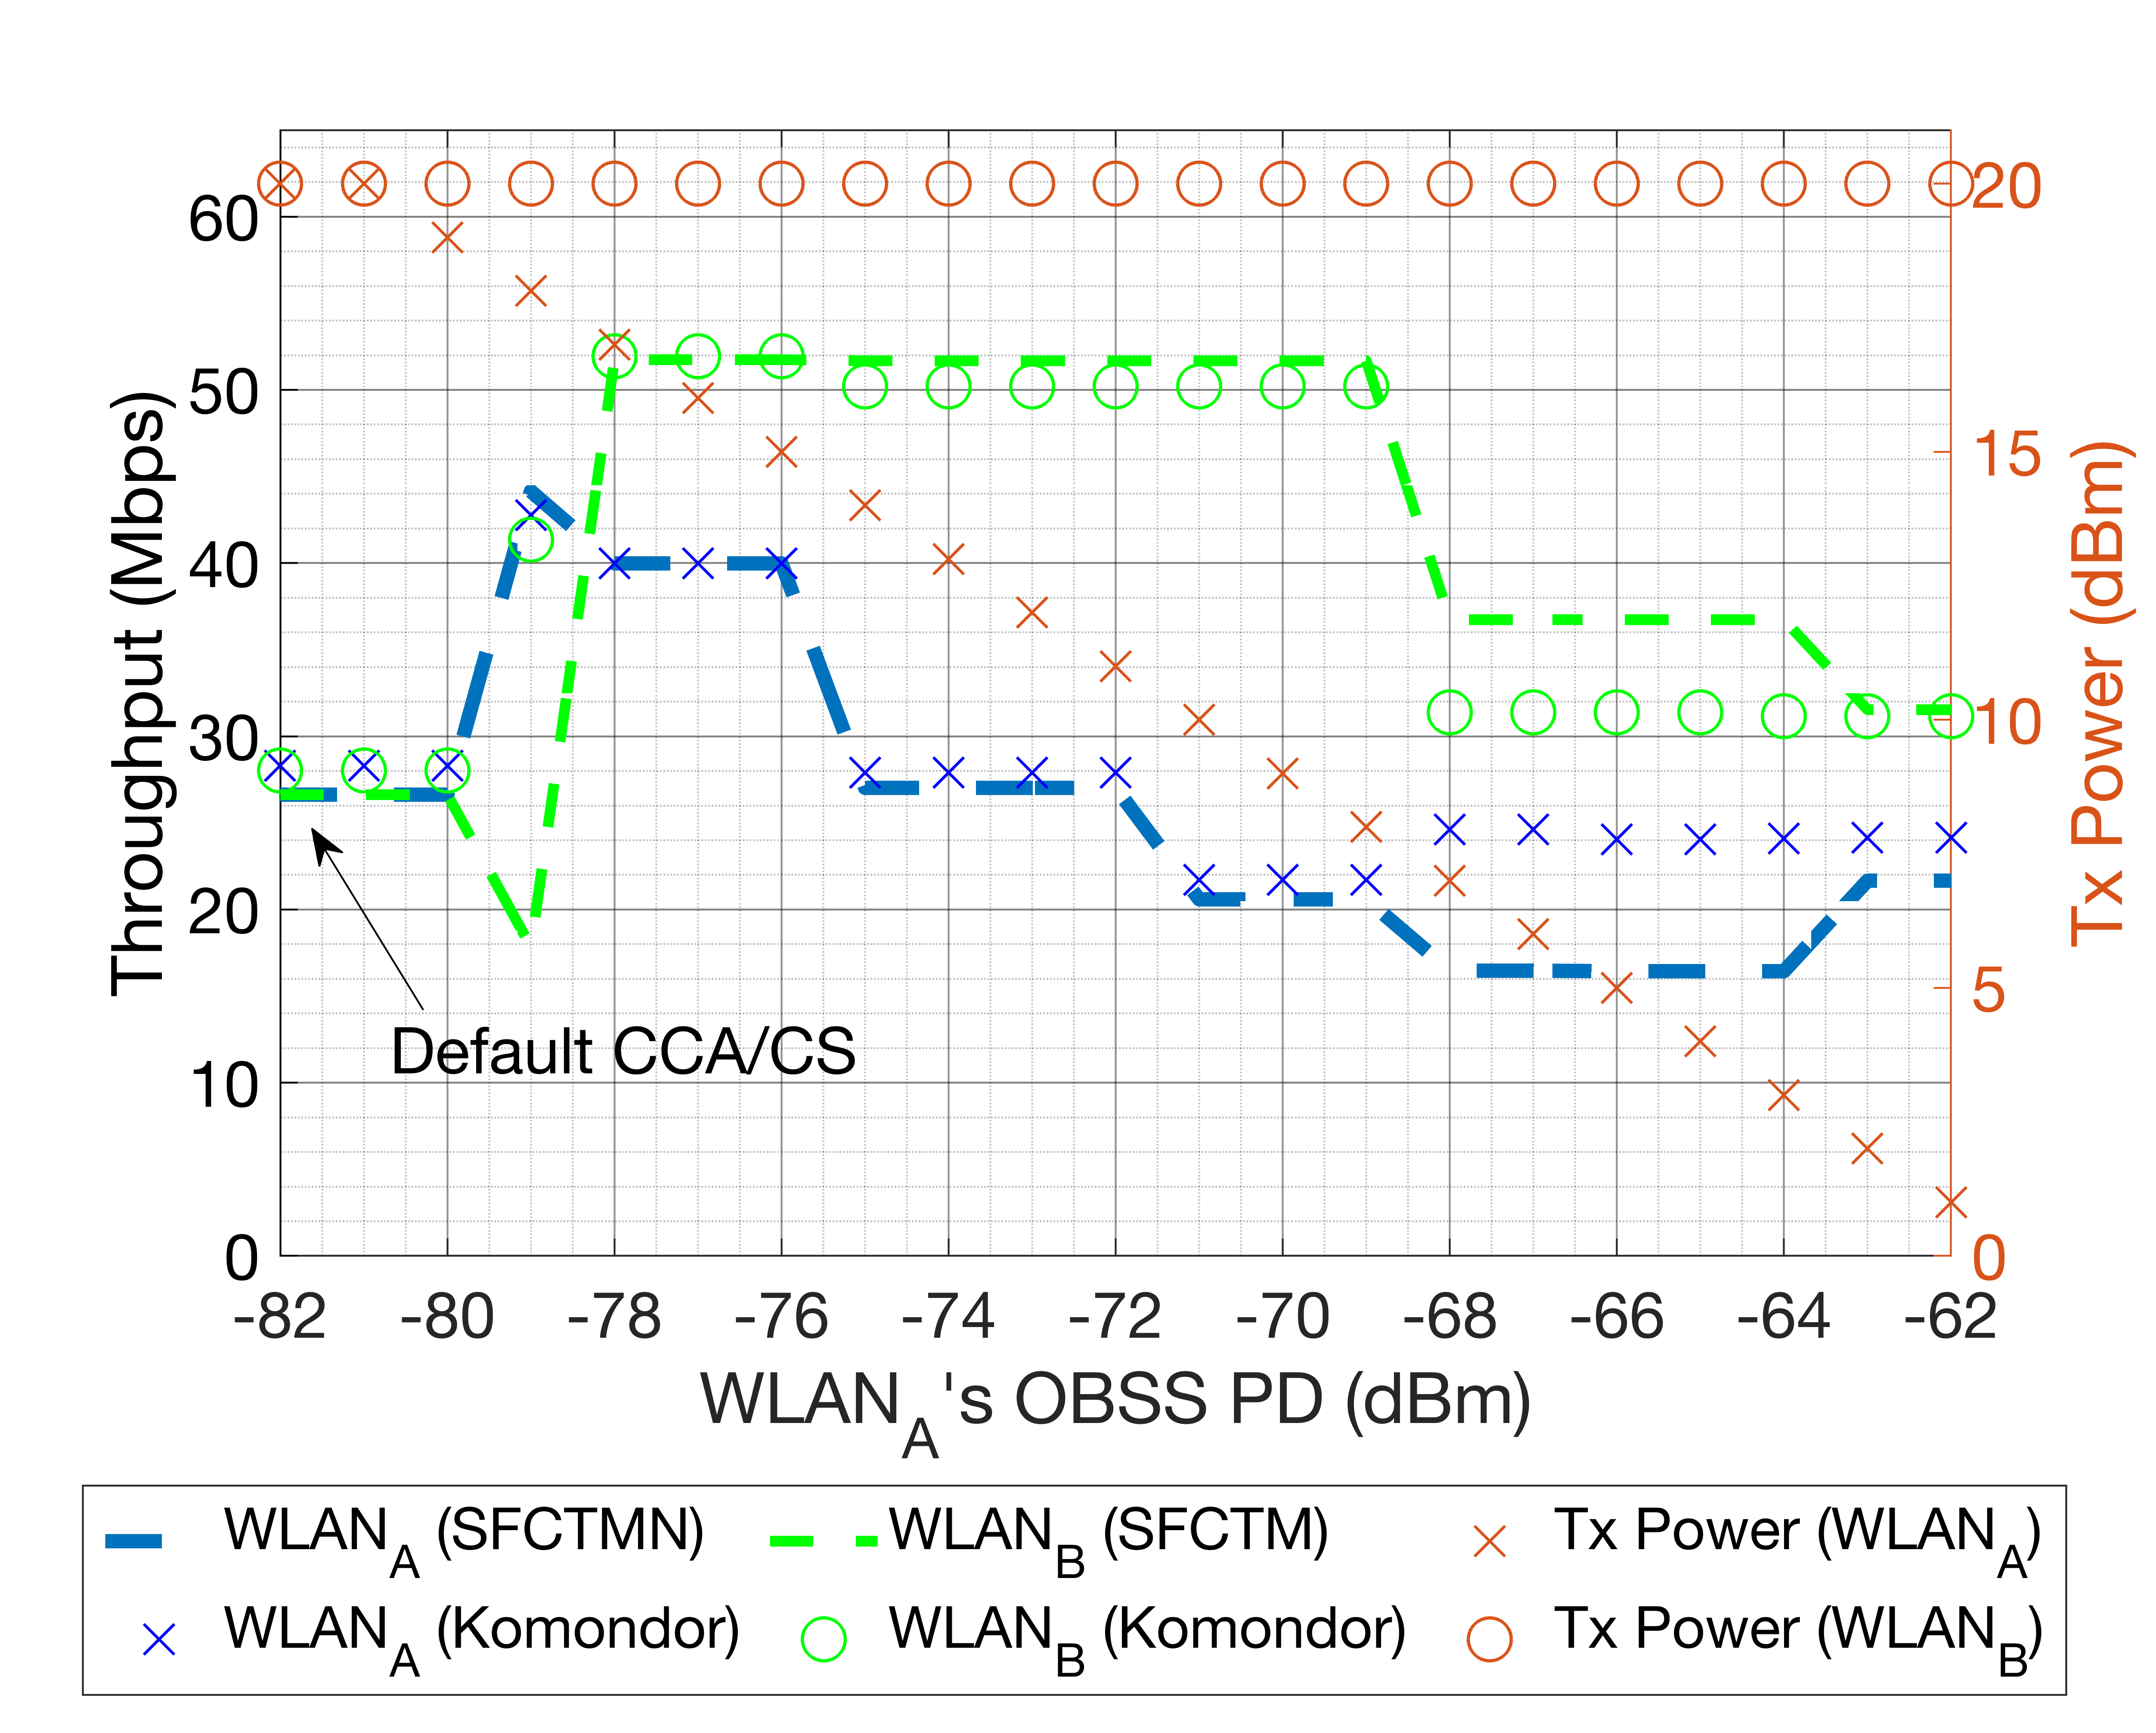
\includegraphics[width=0.6\columnwidth]{SIM_1_1}
	\caption{Effects of applying OBSS/PD-based SR in $\text{BSS}_A$ of \emph{Toy scenario 1}, for each possible OBSS/PD value. The transmission power is shown in red. Results are shown for both SFCTMN and Komondor.}		\label{fig:toy_scenario_1_results}
\end{figure}

As shown, both BSSs obtain the same performance for OBSS/PD $<$ -79 dBm (they share the channel). To that point onwards, $\text{BSS}_A$ is able to ignore $\text{BSS}_B$'s transmissions due to the SR operation. However, what might seem a worthy strategy for $\text{BSS}_A$ turns out to be more beneficial to $\text{BSS}_B$. The latter, except for OBSS/PD = -79 dBm,\footnote{At that point, the transmission power limitation for OBSS/PD = -79 dBm is insufficient, so $\text{BSS}_B$ senses the channel busy when $\text{BSS}_A$ transmits under the SR mode.} enjoys the highest possible throughput when $\text{BSS}_A$ applies the SR operation. The fact is that $\text{BSS}_A$ is forced to use a lower transmission power in case of transmitting when $\text{BSS}_B$ is occupying the channel. Therefore, $\text{BSS}_B$ will keep sensing the channel idle once its transmission finishes, provided that $\text{BSS}_A$ is still subject to the transmission power restriction.

It is important to note that, in Fig. \ref{fig:toy_scenario_1_results}, there is a region (from OBSS/PD = -68 dBm to OBSS/PD = -64 dBm, both included) in which the SFCTMN is less accurate at capturing the actual OBSS behavior on using SR. For these OBSS/PD values, $\text{STA}_A$ cannot decode any transmission from $\text{AP}_A$ in state $A_\text{SR}B$. In turn, it can do that for the $A_\text{SR}$ state. In particular, the transmit power limitation used by $\text{AP}_A$ in the SR mode makes that $\text{STA}_A$ perceives an insufficient signal-to-noise-plus-interference ratio (SINR) when $\text{BSS}_B$ is also occupying the channel. The main reason is that the SFCTMN model considers that the throughput obtained in every state is independent of the others, and this condition does not hold for states $A_\text{SR}B$ and $A_\text{SR}$. In reality, $\text{AP}_A$ is expected to abandon its transmission in state $A_\text{SR}B$ as soon as a timeout is noticed, thus spending a few time in the SR mode (transition $A_\text{SR}B$ to $A_\text{SR}$ is unlikely). In contrast, the SFCTMN considers that much more time is spent in state $A_\text{SR}$ since transmissions at that point are successful (but slow due to the low MCS used).

Now, let us consider the case where both BSSs apply the SR operation simultaneously. The CTMN for OBSS/PD $\geq$ -79 dBm is shown in Fig. \ref{fig:ctmn_toy_scenario_1c}. For the sake of illustration, only transitions between states $s_0$ and $s_1$ are provided. As shown, both BSSs can act by using the default or the SR modes, thus generating a symmetric CTMN. In particular, we find two dominant states: $s_5$  and $s_6$. These states are visited with the same probability (0.4482), which indicates that both BSSs alternate the default and the SR modes, thus obtaining the same throughput. However, in reality, one of the BSSs may monopolize the channel through under the default mode, while the other operates under the transmit power-constrained SR mode. 

\begin{figure}[ht!]
	\centering    
	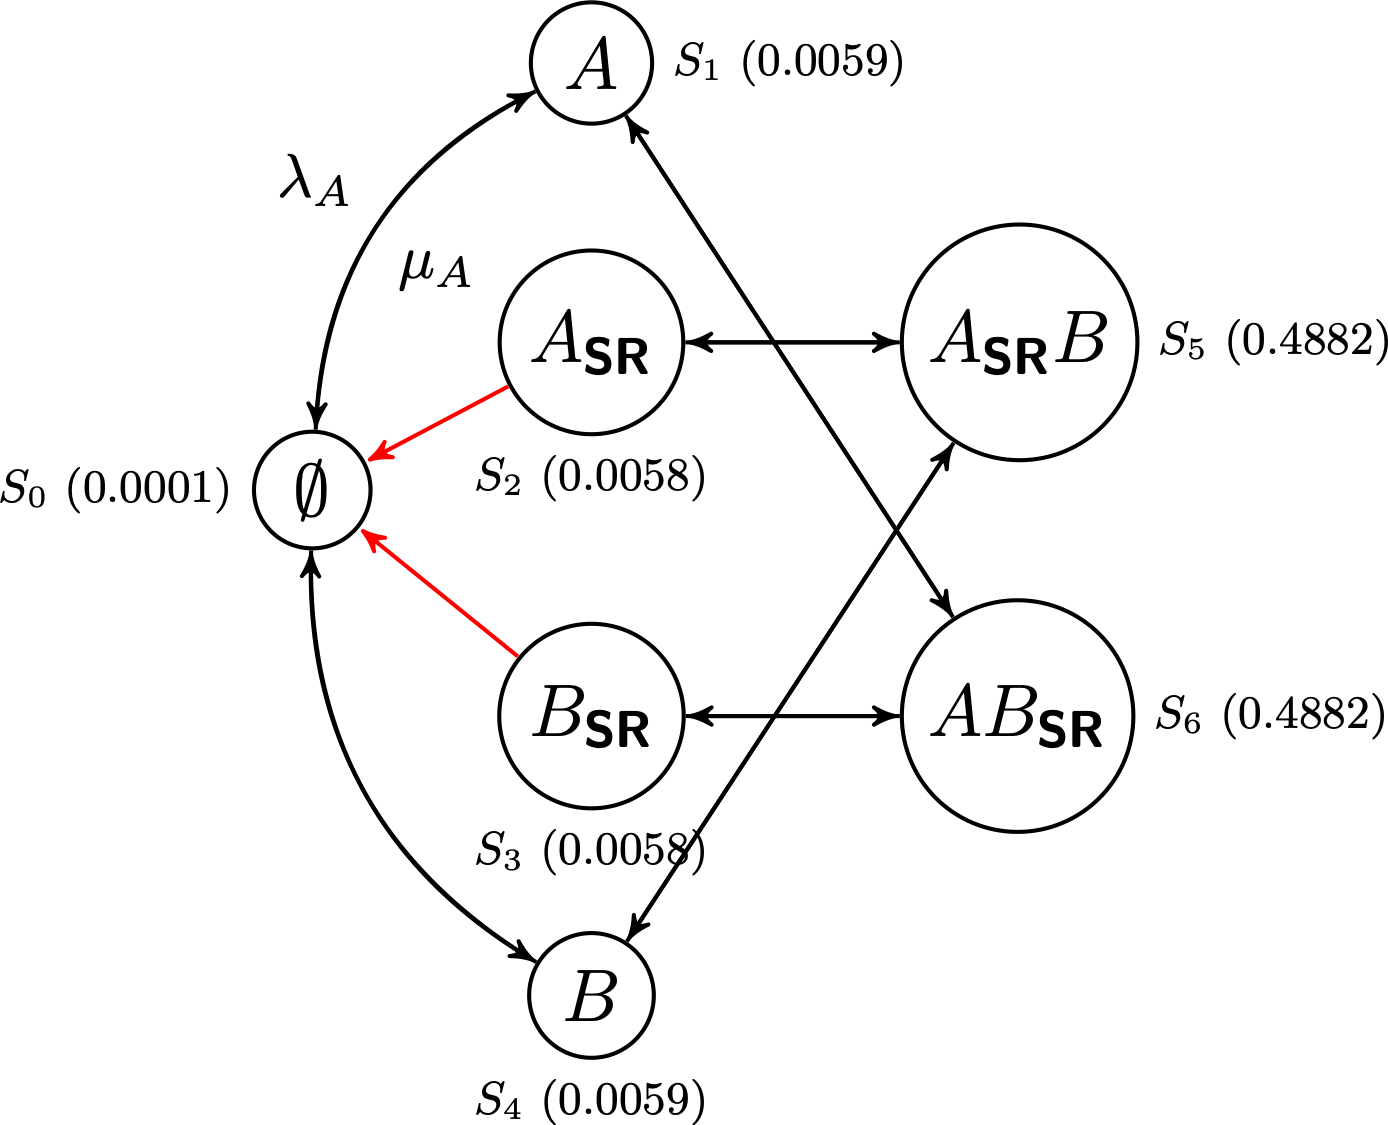
\includegraphics[width=.6\textwidth]{ctmn_toy_scenario_1c}
	\caption{CTMN of \emph{Toy scenario 1} when both BSSs apply OBSS/PD-based SR with OBSS/PD~$\geq$~-79~dBm (unidirectional transitions are marked in red).}
	\label{fig:ctmn_toy_scenario_1c}
\end{figure}

This phenomenon is properly captured in the Komondor simulator, where SR opportunities are identified on a per-packet basis. In this case, the BSS that accesses to the channel for the first time (e.g., $\text{BSS}_A$) is most likely to enjoy the maximum throughput. In contrast, the other BSS (e.g., $\text{BSS}_B$) transmits under the SR mode almost all the time (as a result of $\text{BSS}_A$'s activity), until they alternate roles. Notice that a single state between $s_5$  and $s_6$ is more likely to be monopolized as the transmission time becomes longer than the idle periods. In our case, we have very long transmission times in comparison to the idle time since we assume full-buffer traffic, packet aggregation, and short contention window (CW) values.

%\begin{figure}[ht!]
%	\centering
%	\subfigure[CTMN representation]{\label{fig:ctmn_toy_scenario_1c}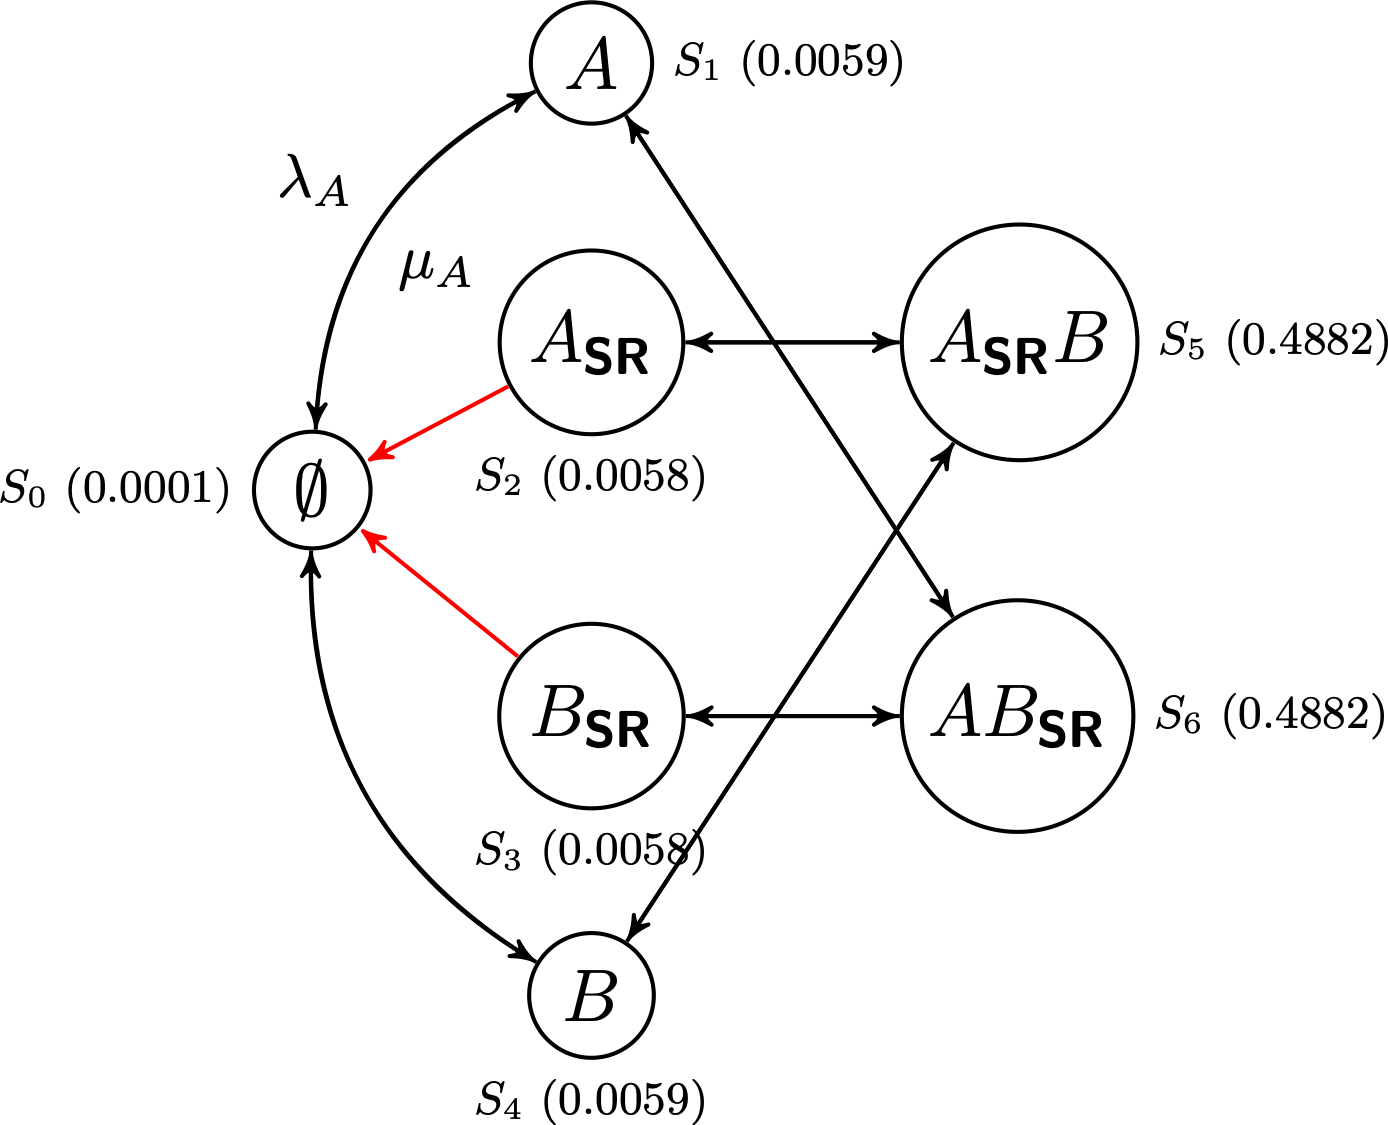
\includegraphics[width=.9\textwidth]{ctmn_toy_scenario_1c}}
%	\subfigure[Throughput]{\label{fig:toy_scenario_1c_results}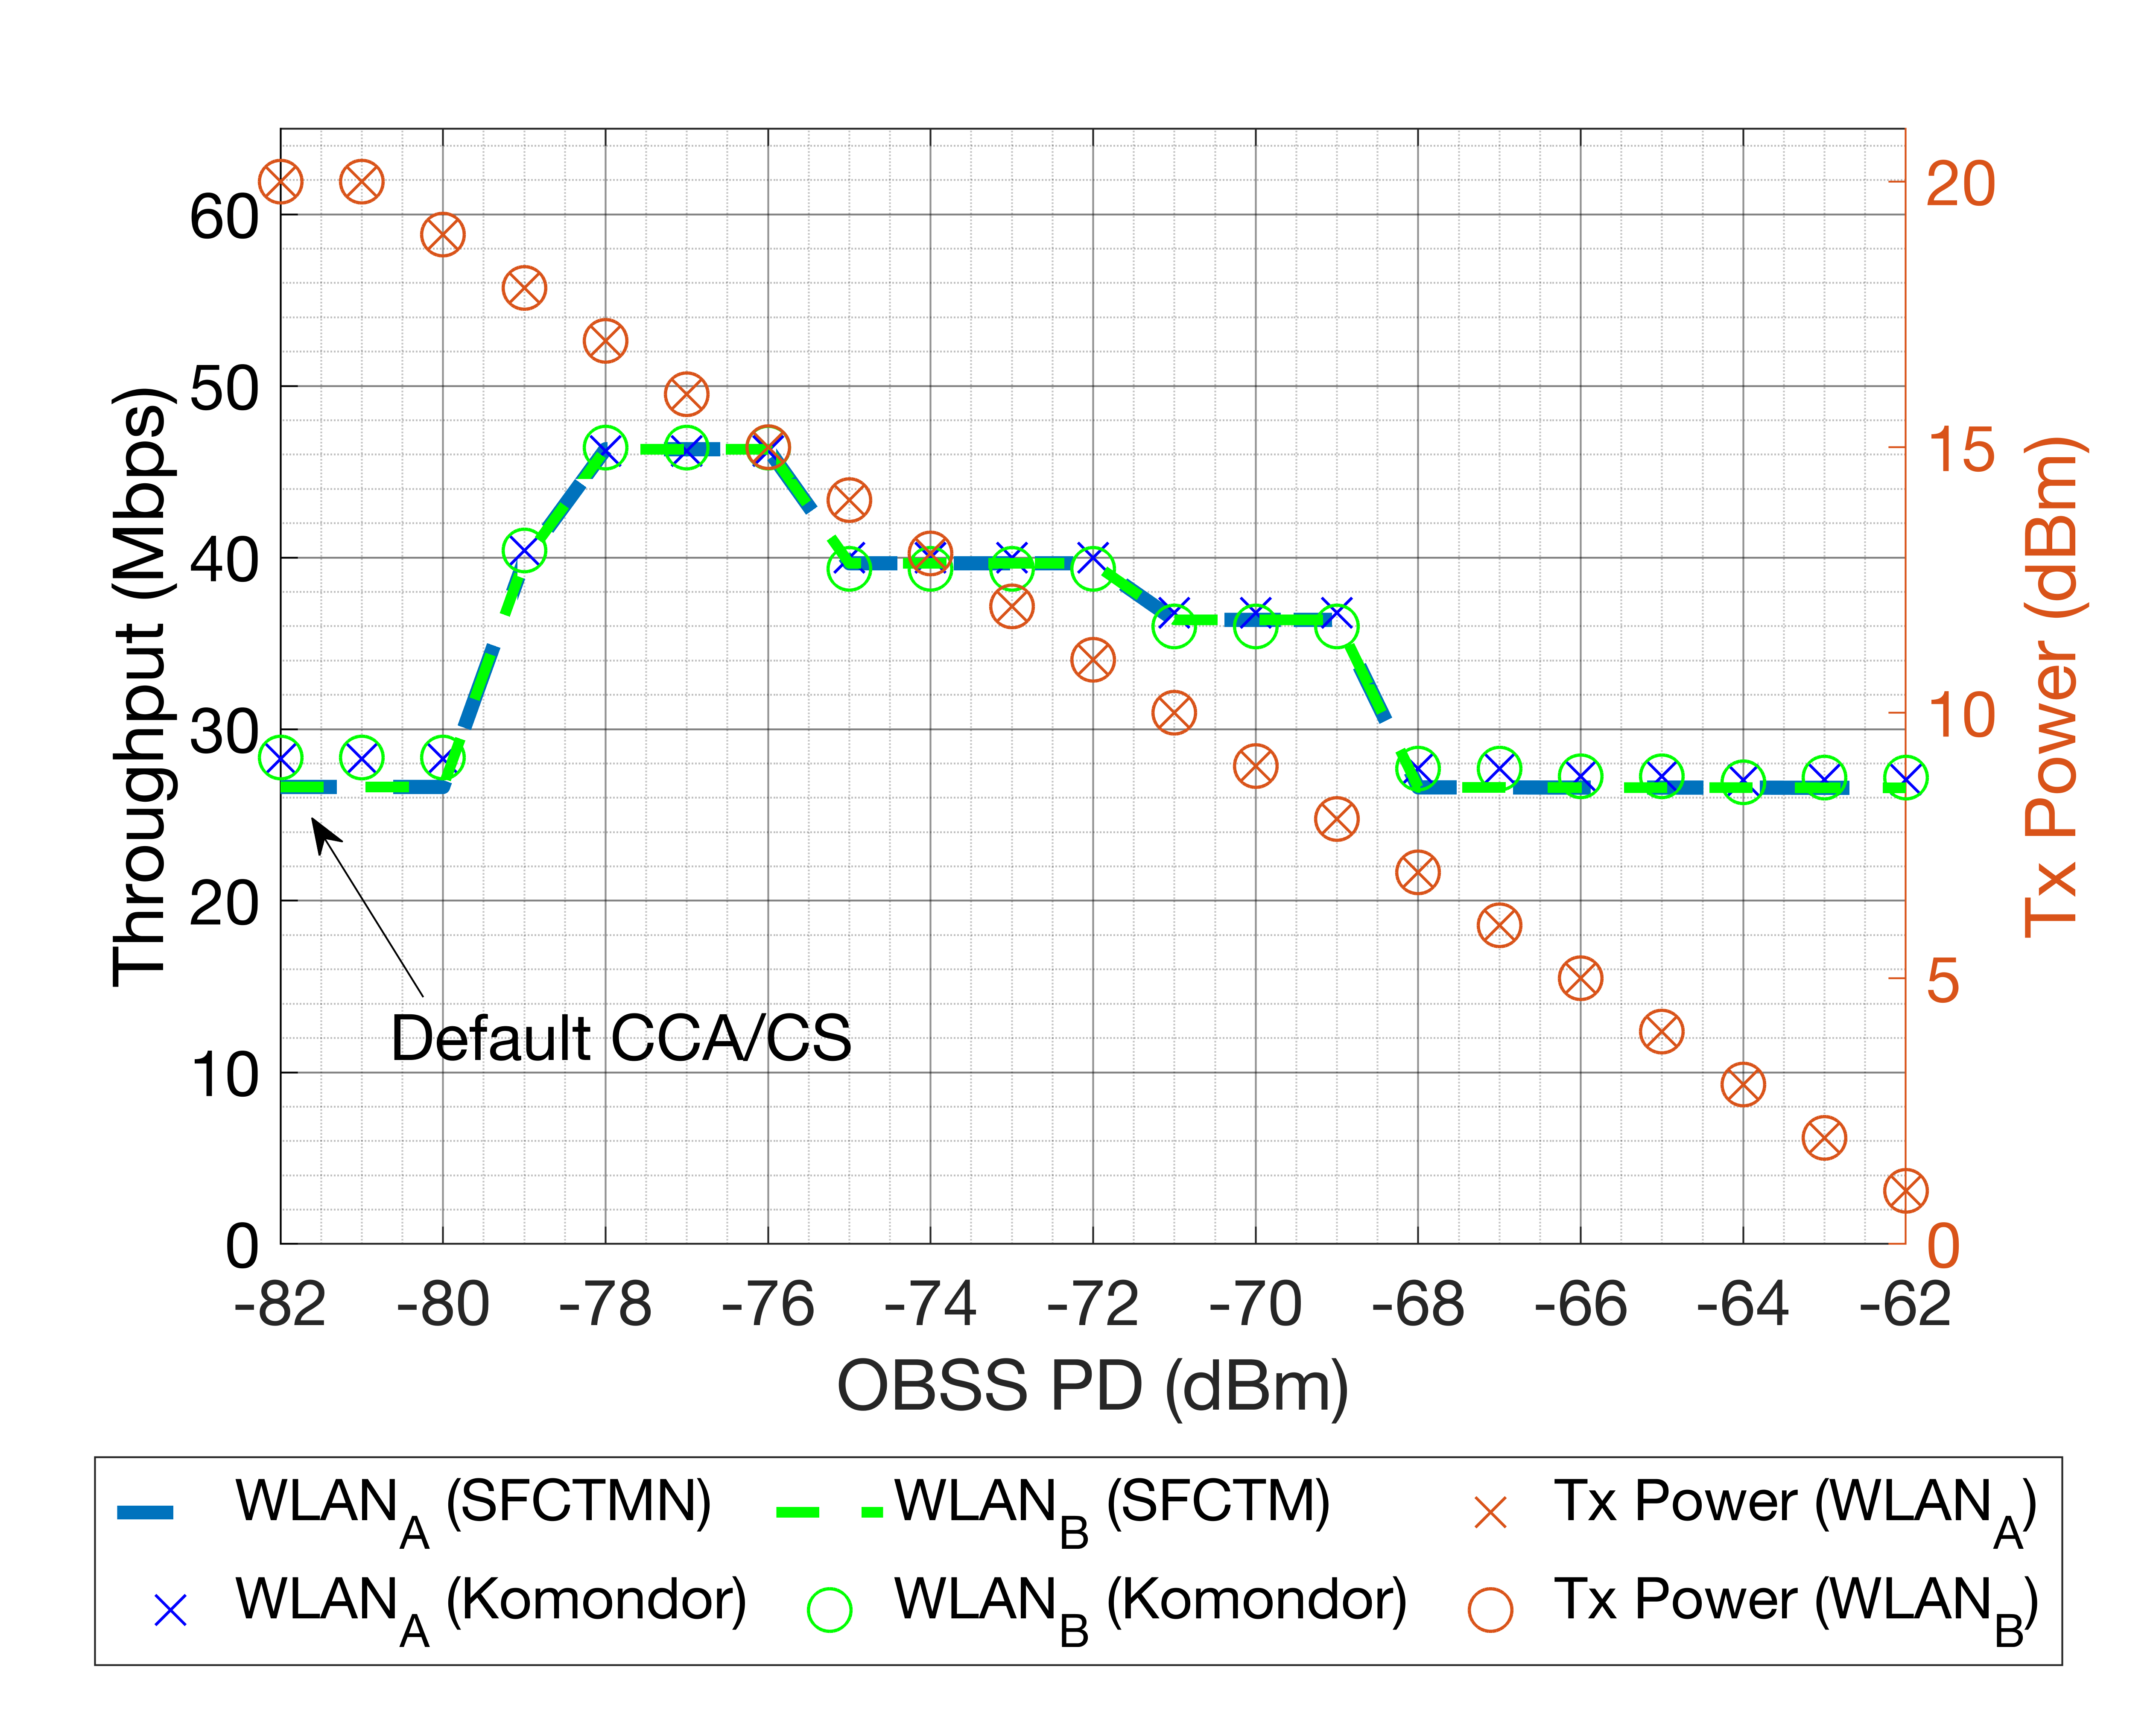
\includegraphics[width=\columnwidth]{SIM_1_1b}}
%	\caption{Effects of applying OBSS/PD-based SR in both BSSs of \emph{Toy scenario 1}. (a) CTMN for OBSS/PD~$\geq$~-79~dBm (unidirectional transitions are marked in red), and (b) throughput obtained for each OBSS/PD value. In (b), the transmission power is shown in red, and results are shown for both SFCTMN and Komondor.}
%	\label{fig:toy_scenario_1c}
%\end{figure}

Fig. \ref{fig:toy_scenario_1c_results} shows the throughput achieved by each BSS when both apply SR, and for each OBSS/PD threshold. Again, the results have been extracted from both SFCTMN and Komondor. In order to show the long-term performance of each BSS in the Komondor simulator, we have displayed the average values obtained from 100 simulations. As shown, the performance achieved by both BSSs is totally fair, due to the symmetry of the scenario. In particular, states in which SR is used are alternated, thus allowing each BSS to access the channel while the other is transmitting. As a result, the throughput of both BSSs can be further increased with respect to the case in which only one BSS applies SR. However, unlike the previous case, the long-term throughput never reaches the maximum possible throughput in isolation (the transmission power limitation prevents to do so).

\begin{figure}[ht!]
	\centering
	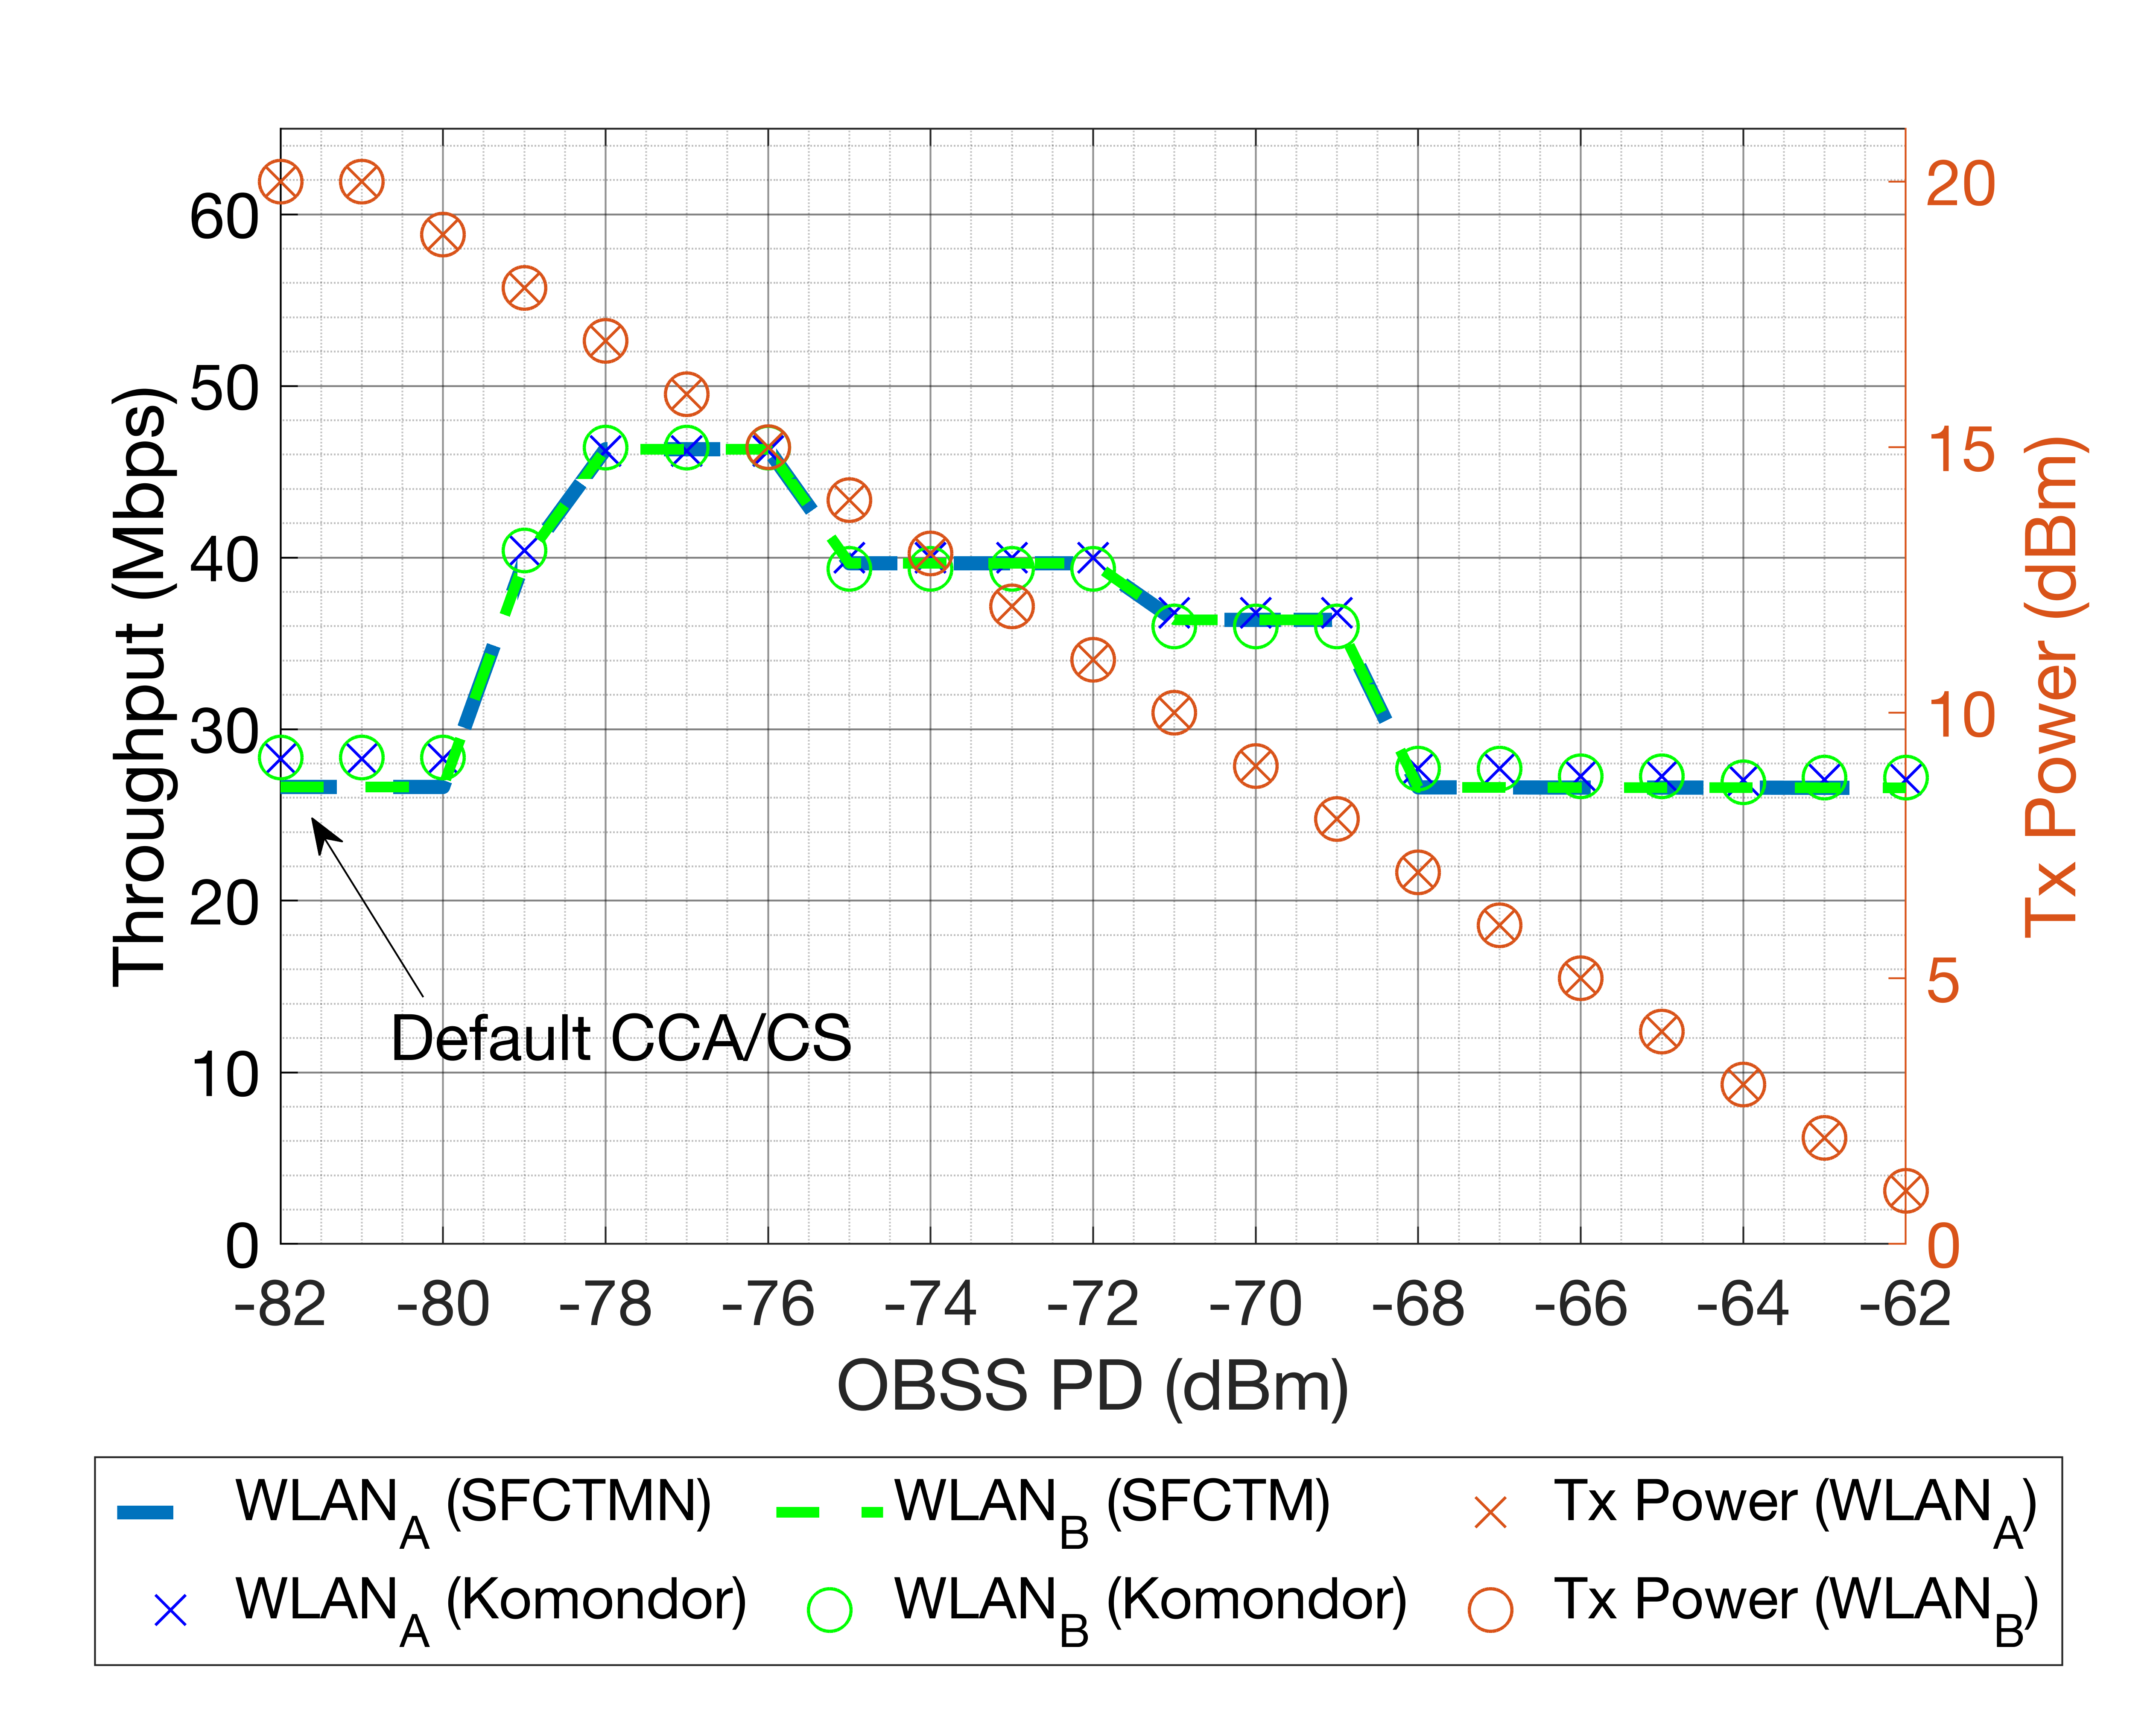
\includegraphics[width=.6\columnwidth]{SIM_1_1b}
	\caption{Effects of applying OBSS/PD-based SR in both BSSs of \emph{Toy scenario 1}, for each possible OBSS/PD value. The transmission power is shown in red. Results are shown for both SFCTMN and Komondor.}		
	\label{fig:toy_scenario_1c_results}
\end{figure}

%%% Complex OBSS/PD-based interactions
\subsection{Interactions among Spatial Reuse groups}
\label{section:advanced_interactions}
Differentiating between SRGs may potentially enhance spectral efficiency due to the further inter-AP interactions that can be generated with an additional OBSS/PD threshold. In practice, devices belonging to the same SRG use a dedicated OBSS/PD threshold, namely SRG OBSS/PD. For the rest of inter-BSS transmissions, the non-SRG OBSS/PD threshold is used instead. One possible use case may lie in residential building apartments, where BSSs belonging to the same building form an SRG. For the rest of networks (e.g., public Wi-Fi in the street), other SRGs can be considered.

To illustrate the implications of using SR based on SRGs, let us focus on \emph{Toy scenario 2}, which is depicted in Fig. \ref{fig:toy_scenario_2}. In this deployment, all the BSSs apply the SR operation and two different SRGs are created. In particular, BSSs belonging to the same SRG (i.e., $\text{BSS}_A$ and $\text{BSS}_B$) are close to each other, such as in a residential building. Apart from that, $\text{BSS}_C$, belongs to another SRG. 

\begin{figure}[ht!]
	\centering
	\subfigure[Scenario]{\label{fig:toy_scenario_2}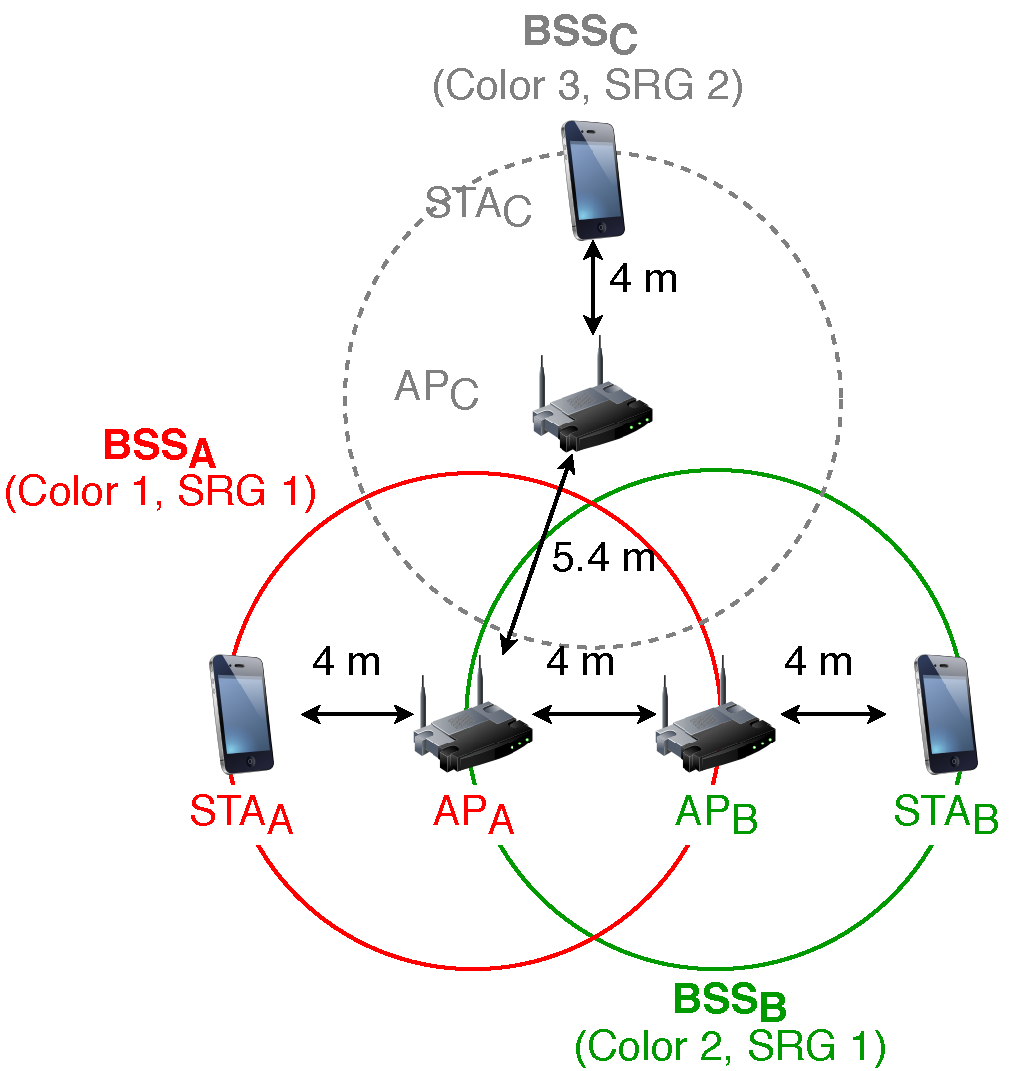
\includegraphics[width=0.38\textwidth]{fig_18}}%
	\hspace{1cm}%
	\subfigure[Results]{\label{fig:SIM_1_3_individual}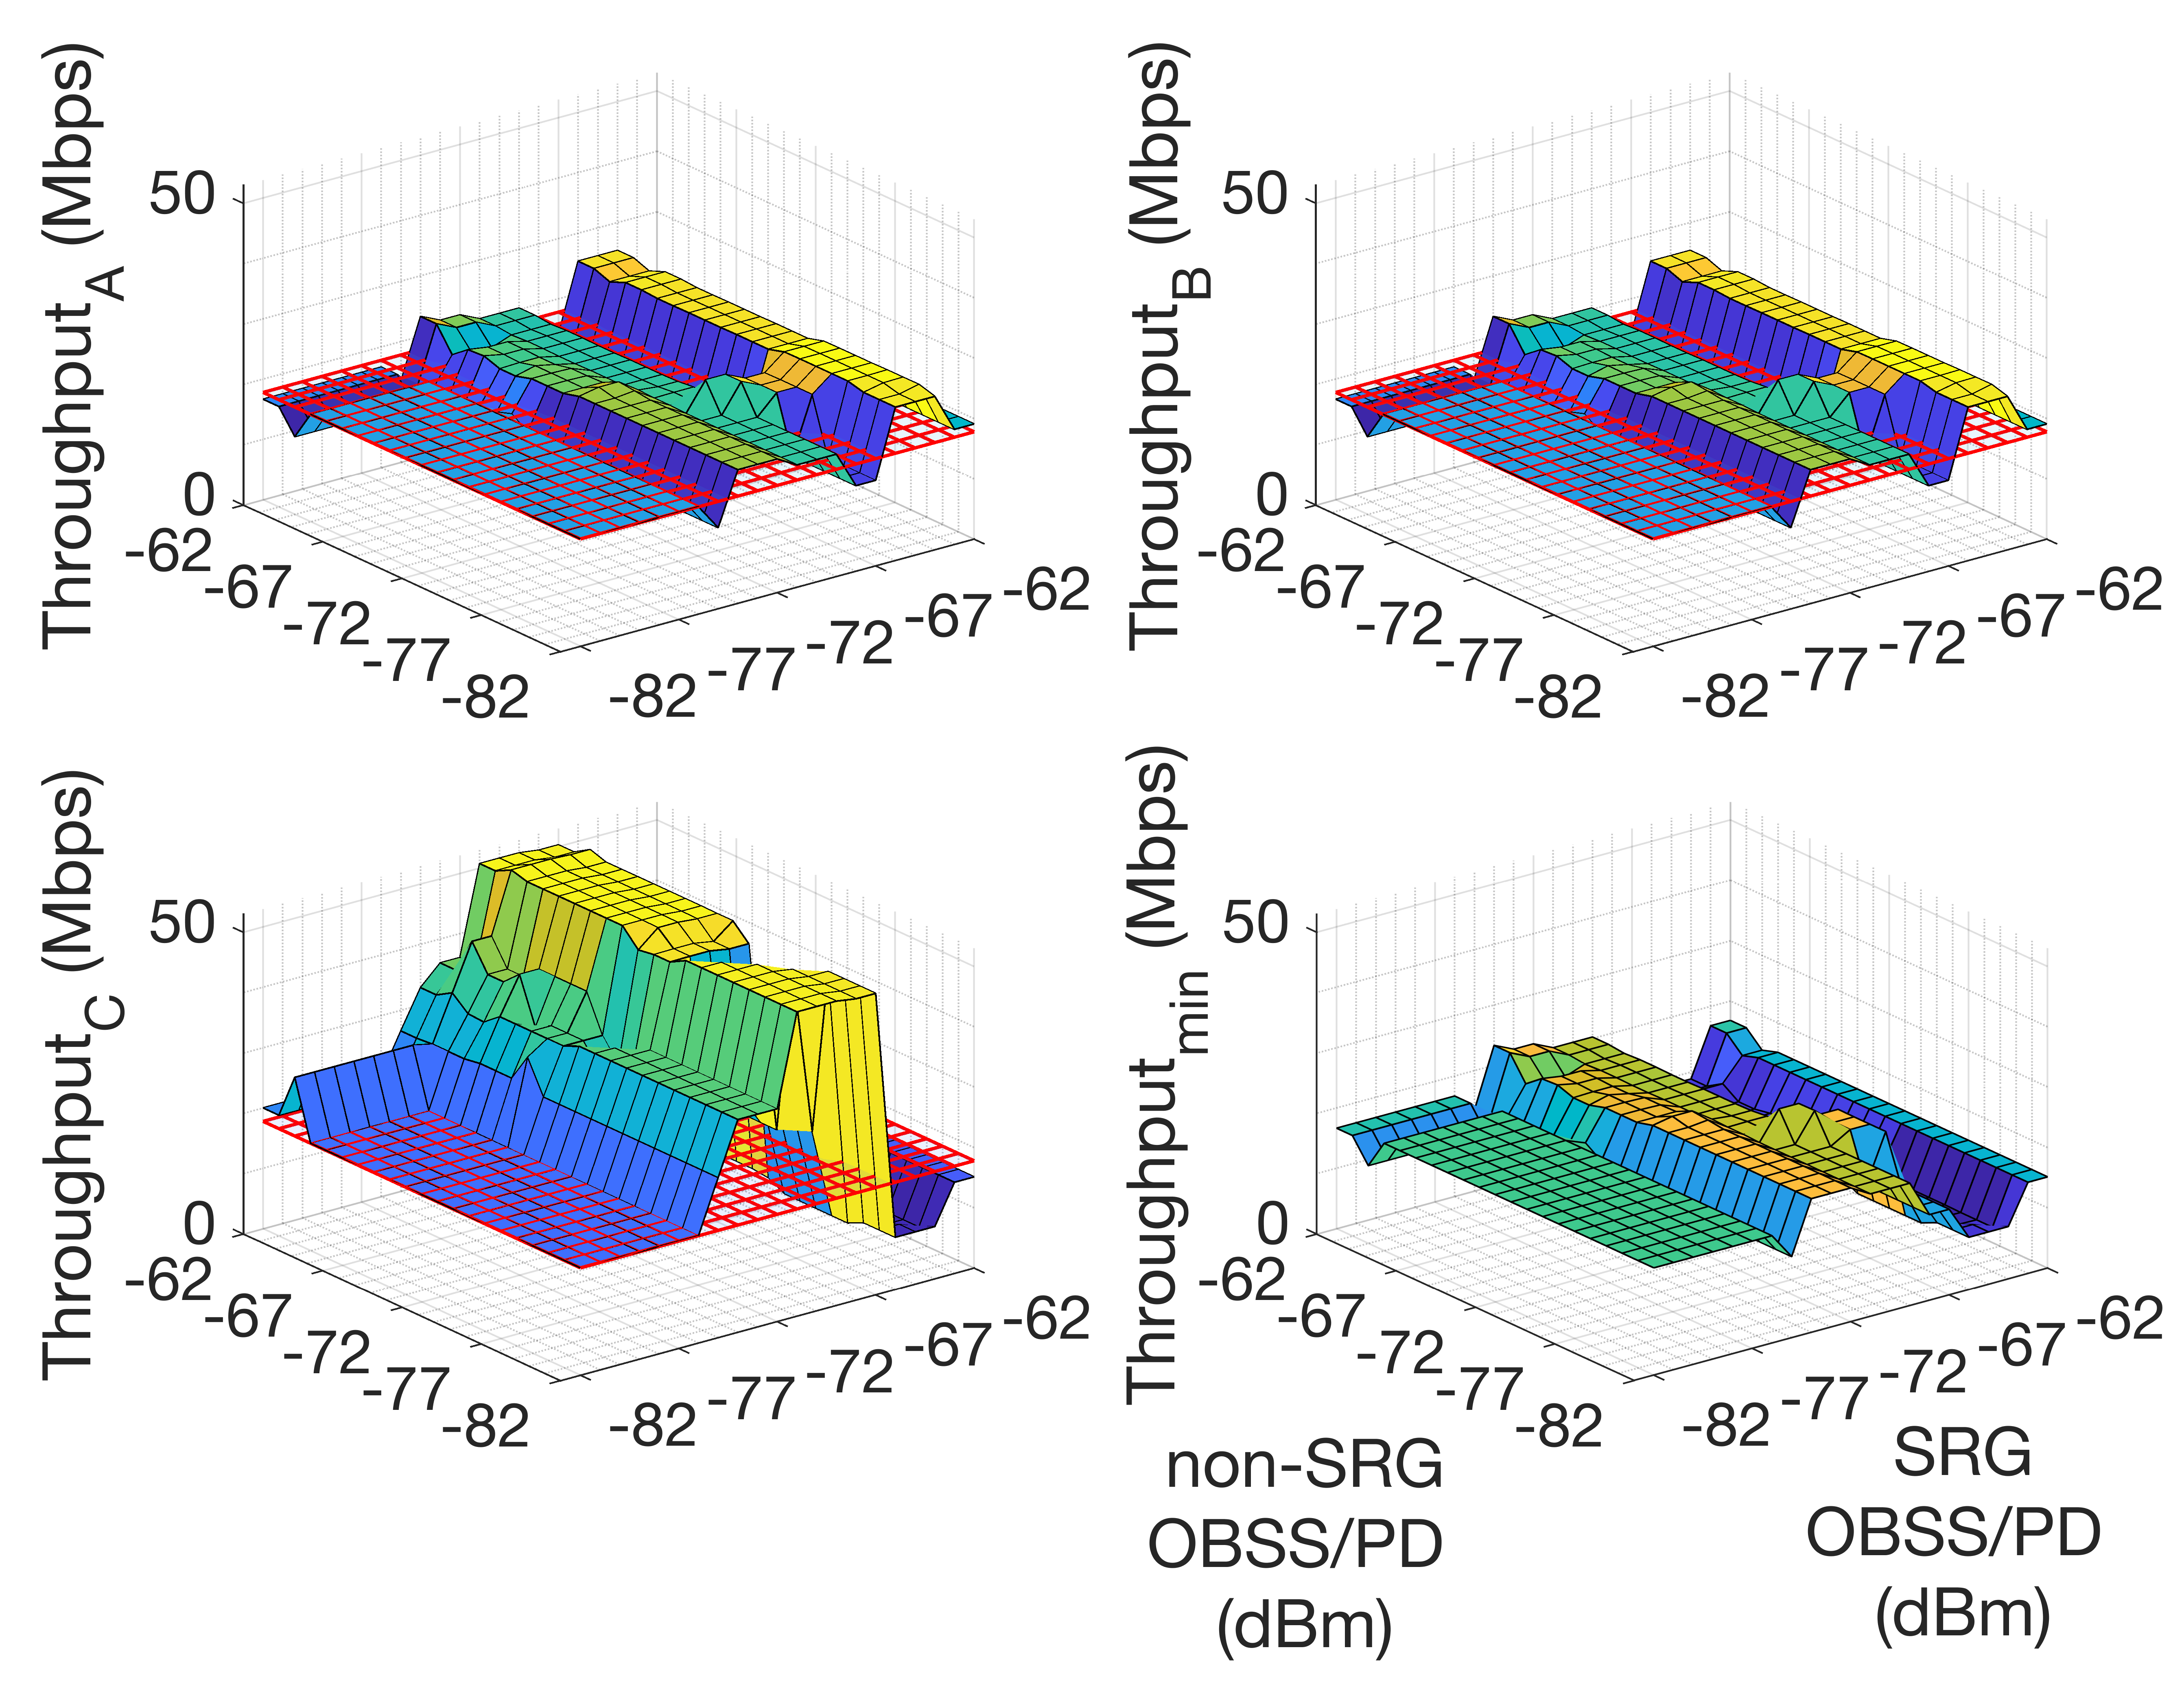
\includegraphics[width=.52\columnwidth]{SIM_1_2}}
	\caption{Results of applying the OBSS/PD-based SR operation in \emph{Toy scenario 2}. In (b), the individual and max-min throughput are shown for each SRG and non-SRG OBSS/PD threshold. The red mesh indicates the performance achieved by using the default CCA/CS.}
	\label{fig:fig:17}
\end{figure}

The result of jointly applying OBSS/PD-based SR in \emph{Toy scenario 2} is illustrated in Fig. \ref{fig:SIM_1_3_individual}, which plots the throughput achieved by each of the three BSSs, for each combination of SRG and non-SRG OBSS/PD thresholds. Notice that we have considered that all the BSSs use the same OBSS/PD values since the number of total combinations grows exponentially and is unfeasible to be plotted.

As shown, the throughput achieved by each BSS follows an irregular pattern due to the complex inter-BSS interactions that take place in this scenario. Moreover, it can be appreciated the clashing interests of each BSS, where the individual performance is sometimes maximized at the expense of reducing the throughput of the others. For instance, if we focus on $\text{BSS}_C$, it obtains the maximum throughput when flow starvation is generated to $\text{BSS}_A$ (the same occurs for $\text{BSS}_B$). However, this is not optimal in terms of fairness. The CTMN resulting from the flow starvation situation is shown in Fig. \ref{fig:ctmn_scenario_2}, which is given when all the BSSs use non-SRG OBSS/PD = -82 dBm and SRG OBSS/PD = -73 dBm.\footnote{The CTMN model captures the utilization of different OBSS/PD thresholds by considering that each BSS acts in three different ways (states), as a result of the employed OBSS/PD threshold: \emph{i)} default CCA/CS, \emph{ii)} SRG OBSS/PD, and \emph{iii)} non-SRG OBSS/PD.}

In case of considering the optimal max-min performance\footnote{The max-min throughput corresponds to the solution that maximizes the minimum throughput achieved by a set of BSSs.}, a completely different situation is observed. In this case, the max-min throughput is increased when every BSS can overtake a single detected inter-BSS transmission (regardless of its source) and access to the channel. This situation is fair and at the same time increases the overall performance. However, it occurs when all the inter-BSS transmissions are equally treated. Using SRGs can therefore improve the performance of certain nodes (belonging to the same group), but potentially leads to unfairness. 
\begin{figure}[ht]
	\centering
	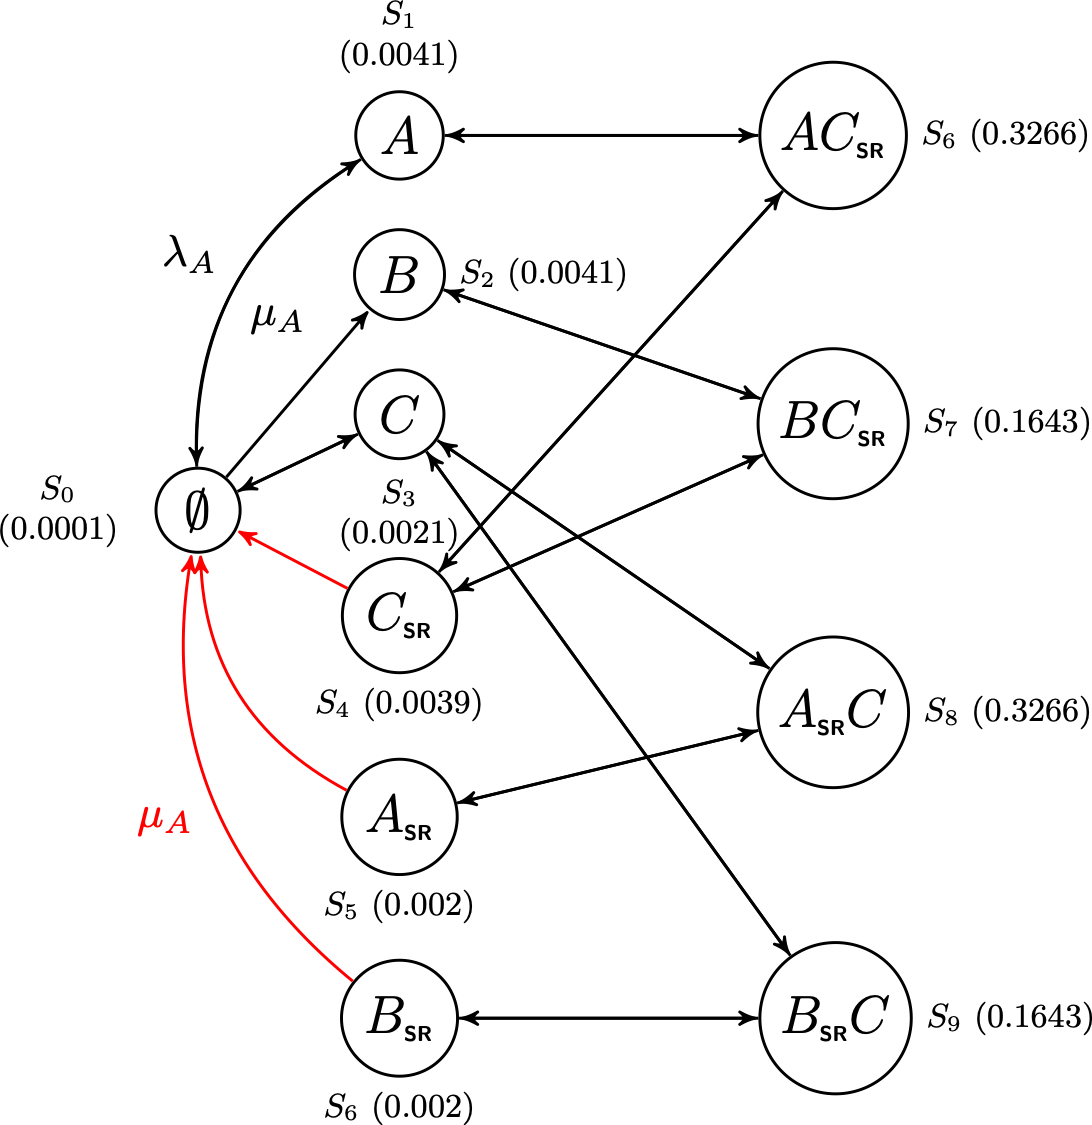
\includegraphics[width=.5\textwidth]{ctmn_scenario_2}
	\caption{CTMN of \emph{Toy scenario 2}, for non-SRG OBSS/PD = -73 dBm and SRG OBSS/PD = -82 dBm. The unidirectional transitions are marked in red, and subindex \emph{SR} indicates the use of the non-SRG OBSS/PD threshold.}
	\label{fig:ctmn_scenario_2}
\end{figure}

Table \ref{tbl:cross_validation} provides a verification, for both SFCTMN and Komondor, of the results obtained in \emph{Toy scenario 2}. For the sake of representation, we show the Root Mean Square Error (RMSE) for all the considered SRG and non-SRG OBSS/PD threshold values. As shown, the error for $\text{BSS}_A$ and $\text{BSS}_B$ is relatively small. In contrast, a higher error is obtained for $\text{BSS}_C$. This is strongly related to the fact that $\text{BSS}_C$ belongs to a different SRG than $\text{BSS}_A$ and $\text{BSS}_B$, which leads to different inter-BSS interactions. Moreover, dominant states may lead to situations that cannot be captured by the SFCTMN, as previously shown for \emph{Toy scenario 1}. In particular, $\text{BSS}_C$ in \emph{Toy scenario 2} is prone to participate in these states because of its asymmetric location with respect to $\text{BSS}_A$ and $\text{BSS}_B$.
\begin{table}[ht!]
	\centering
	\resizebox{0.4\textwidth}{!}{	
	\begin{tabular}{|c|c|c|c|}
		\hline
		& $\text{BSS}_A$ & $\text{BSS}_B$ & $\text{BSS}_C$ \\ \hline
		\begin{tabular}[c]{@{}c@{}}RMSE \\ (Mbps)\end{tabular} & 6.02 & 6.03 & 18.42 \\ \hline
	\end{tabular}}
	\caption{Verification of the results obtained in \emph{Toy scenario 2} from the SFCTMN and Komondor.}
	\label{tbl:cross_validation}
\end{table}

% ----------------------------------
% -
% 	-- Performance Evaluation --
% -
% ----------------------------------

\section{Performance Evaluation}
\label{section:performance_evaluation}

In this Section, we study the potential gains of SR in large-scale WLAN scenarios. With this aim, we leave the CTMNs-based analysis out and concentrate on simulation results. For the rest of this Section, each BSS is considered to be composed by an AP and a single STA, which are placed uniformly at random, as shown in Fig. \ref{fig:random_scenario}. 

\begin{figure}[ht!]
	\centering
	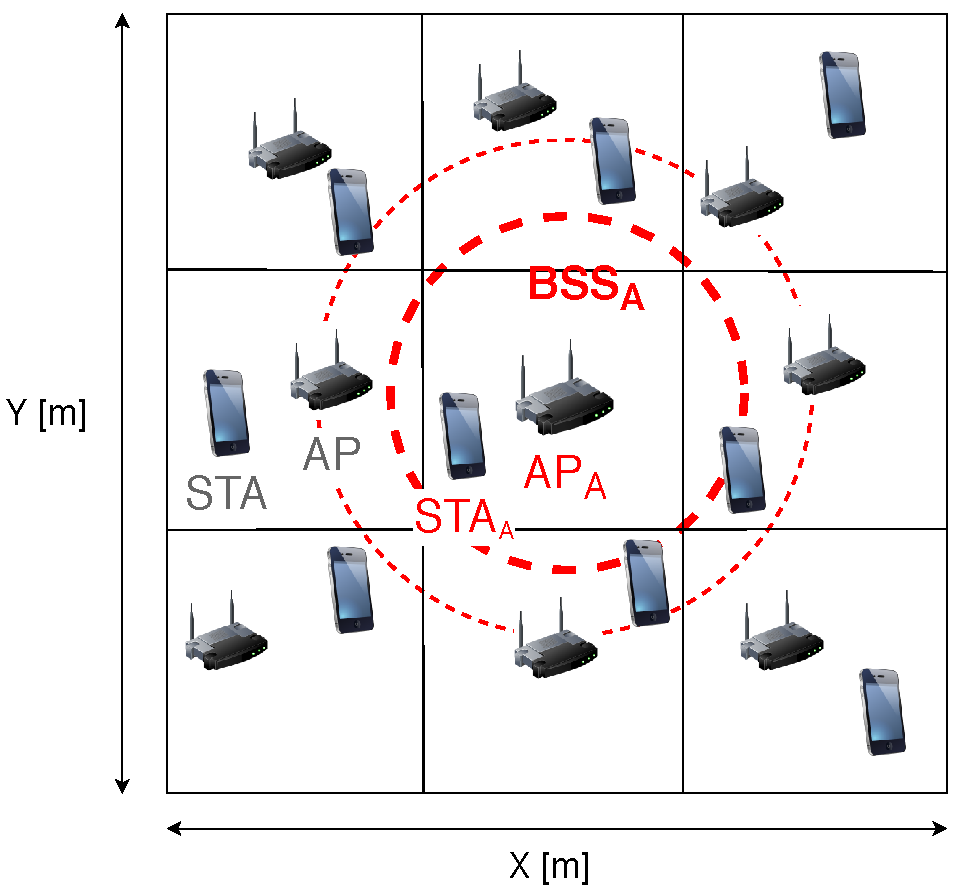
\includegraphics[width=0.5\textwidth]{random_scenario}
	%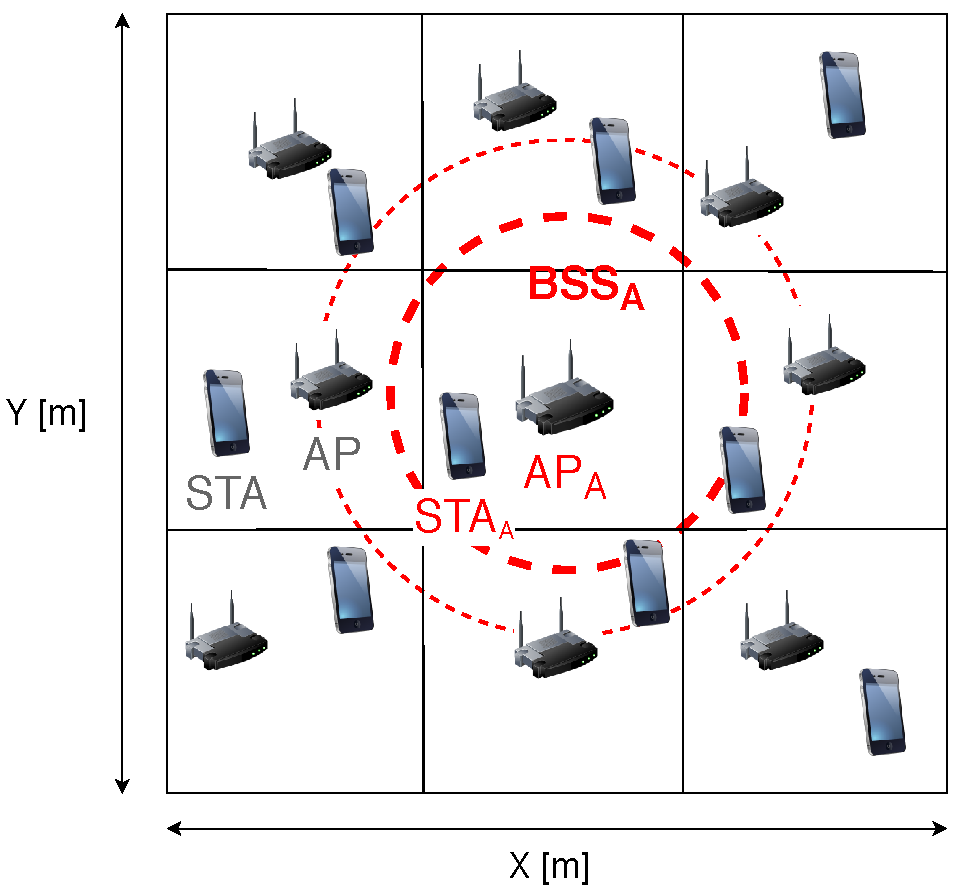
\epsfig{file=random_scenario.pdf, width=5.5cm}
	\caption{Random grid scenario containing 9 BSSs. The location of $\text{BSS}_A$ is fixed at the center for the sake of analysis.}
	\label{fig:random_scenario}
\end{figure}

The simulation parameters are provided in Table \ref{table:parameters}. The scenario is divided into 9 cells, but the location of $\text{BSS}_A$ is always fixed at the center of the scenario. For the rest of the APs and STAs, their position is randomly selected within their corresponding cell. The configuration of each BSS is set homogeneously, i.e., they all use the same channel, the default sensitivity is set to -82 dBm, and the default transmission power is set to 20 dBm. Notice that, for dense deployments, $\text{BSS}_A$ is expected to suffer a higher level of interference than the others, which allows us to assess the effectiveness of the SR operation in crowded environments.

\begin{table}[h]
	\centering
	\resizebox{.8\columnwidth}{!}{
		\begin{tabular}{c|l|l|}
			\cline{2-3}
			\multicolumn{1}{l|}{} & \textbf{Parameter} & \textbf{Value}
			\\ \hline
			% PHY
			\multicolumn{1}{|c|}{\multirow{9}{*}{\rotatebox[origin=c]{90}{PHY}}} & Central frequency, $f_c$ & 5 GHz \\ \cline{2-3} 
			\multicolumn{1}{|c|}{} & Transmission gain, $G_{tx}$ & 0 dB \\ \cline{2-3} 
			\multicolumn{1}{|c|}{} & Reception gain, $G_{rx}$ & 0 dB \\ \cline{2-3} 
			\multicolumn{1}{|c|}{} & Path-loss (residential scenario), $\text{PL}(d)$ & See (\cite{pathloss11ax})  \\ \cline{2-3}
			\multicolumn{1}{|c|}{} & Background noise level, $N$ & -95 dBm \\ \cline{2-3}
			\multicolumn{1}{|c|}{} & Legacy OFDM symbol duration, $\sigma_\text{leg}$ & 4 \textmu s \\
			\cline{2-3}
			\multicolumn{1}{|c|}{} & OFDM symbol duration (GI-32), $\sigma$ & 16 \textmu s \\ 				\cline{2-3}
			\multicolumn{1}{|c|}{} & Number of subcarriers (20 MHz), $N_{sc}$ & 234   \\
			\cline{2-3}
			\multicolumn{1}{|c|}{} & Number of spatial streams, $N_{ss}$ & 1  \\
			\cline{2-3}
			\multicolumn{1}{|c|}{} & Transmit power levels, $\mathcal{T}$ & 1 to 20 dBm (1 dBm steps) \\
			\hline
			% MAC
			\multicolumn{1}{|c|}{\multirow{16}{*}{\rotatebox[origin=c]{90}{MAC}}} & Empty slot duration, $\text{T}_e$ & 9 $\mu$s\\ 
			\cline{2-3} 
			\multicolumn{1}{|c|}{} & SIFS duration, $T_\text{SIFS}$ & 16 \textmu s  \\
			\cline{2-3} 
			\multicolumn{1}{|c|}{} & DIFS/AIFS duration, $T_\text{DIFS/AIFS}$ & 34 \textmu s \\
			\cline{2-3} 
			\multicolumn{1}{|c|}{} & PIFS duration, $T_\text{PIFS}$  & 25 \textmu s \\
			\cline{2-3} 
			\multicolumn{1}{|c|}{} & Legacy preamble duration, $T_\text{PHY-leg}$ & 20 \textmu s  \\
			\cline{2-3}
			\multicolumn{1}{|c|}{} & HE single-user field duration, $T_\text{HE-SU}$ & 100 \textmu s \\
			\cline{2-3} 
			\multicolumn{1}{|c|}{} & ACK duration, $T_\text{ACK}$ & 28 \textmu s\\
			\cline{2-3} 
			\multicolumn{1}{|c|}{} & Block ACK duration, $T_\text{BACK}$ & 32 \textmu s \\
			\cline{2-3} 
			\multicolumn{1}{|c|}{} &  Size OFDM symbol (legacy), $L_{s,l}$ & 24 bits \\
			\cline{2-3} 
			\multicolumn{1}{|c|}{} & Length of data packets, $\text{L}_{d}$ & 12,000 bits \\
			\cline{2-3} 
			\multicolumn{1}{|c|}{} & No. of frames in an A-MPDU, $N_{\text{agg}}$ & 64 \\
			\cline{2-3} 
			\multicolumn{1}{|c|}{} & Length of an RTS packet, $L_\text{RTS}$ & 160 bits \\
			\cline{2-3} 
			\multicolumn{1}{|c|}{} & Length of a CTS packet, $L_\text{CTS}$ & 112 bits \\
			\cline{2-3} 
			\multicolumn{1}{|c|}{} & Length of service field, $L_\text{SF}$ & 16 bits  \\
			\cline{2-3} 
			\multicolumn{1}{|c|}{} & Length of MAC header, $L_\text{MH}$ & 320 bits \\
			\cline{2-3} 
			\multicolumn{1}{|c|}{} & Contention window (fixed), $\text{CW}$ & 15 \\
			\cline{2-3} 
			\multicolumn{1}{|c|}{} & Allowed sensitivity levels, $\mathcal{S}$ & -82 to -62 (1 dBm steps) \\
			\hline
			% Other
			\multicolumn{1}{|c|}{\multirow{2}{*}{\centering\rotatebox[origin=c]{90}{Misc.  }}} & Traffic model, $\Lambda$ & Downlink (UDP)\\
			\cline{2-3} 
			\multicolumn{1}{|c|}{} & Traffic generation ratio, $l$ & 1,000, 2,000, 10,000 pkts/s\\ 
			\cline{2-3} 
			\multicolumn{1}{|c|}{} & Map area (random scenario), $A$ & 625, 400, 225, 100 m$^2$\\
			\hline
	\end{tabular}}
	\caption{Simulation parameters.}
	\label{table:parameters}
\end{table}

%%% DENSITY
\subsection{Network Density}
\label{section:random_scenarios_density}
To analyze SR based on the network density, we consider four different map sizes: sparse ($25\times25$ m), semi-dense ($20\times20$ m), dense ($15\times15$ m) and ultra-dense ($10\times10$ m). For each type of scenario, we provide 50 different deployments, in which APs and STAs are placed uniformly at random within their corresponding cell. $\text{BSS}_A$ is the only one applying the SR operation. Since we compute all the possible OBSS/PD values to be used by $\text{BSS}_A$, each random deployment leads to $21\times4\times50$ = 4,200 different scenarios.

Figure \ref{fig:SIM_2_1} shows the average throughput achieved under the default and SR settings. In particular, we differentiate between the individual throughput of $\text{BSS}_A$ and the average throughput of the other BSSs. For each network density, we have tried all the possible OBSS/PD values and compared the best one to the default CCA/CS.

\begin{figure}[ht!]
	\centering		
	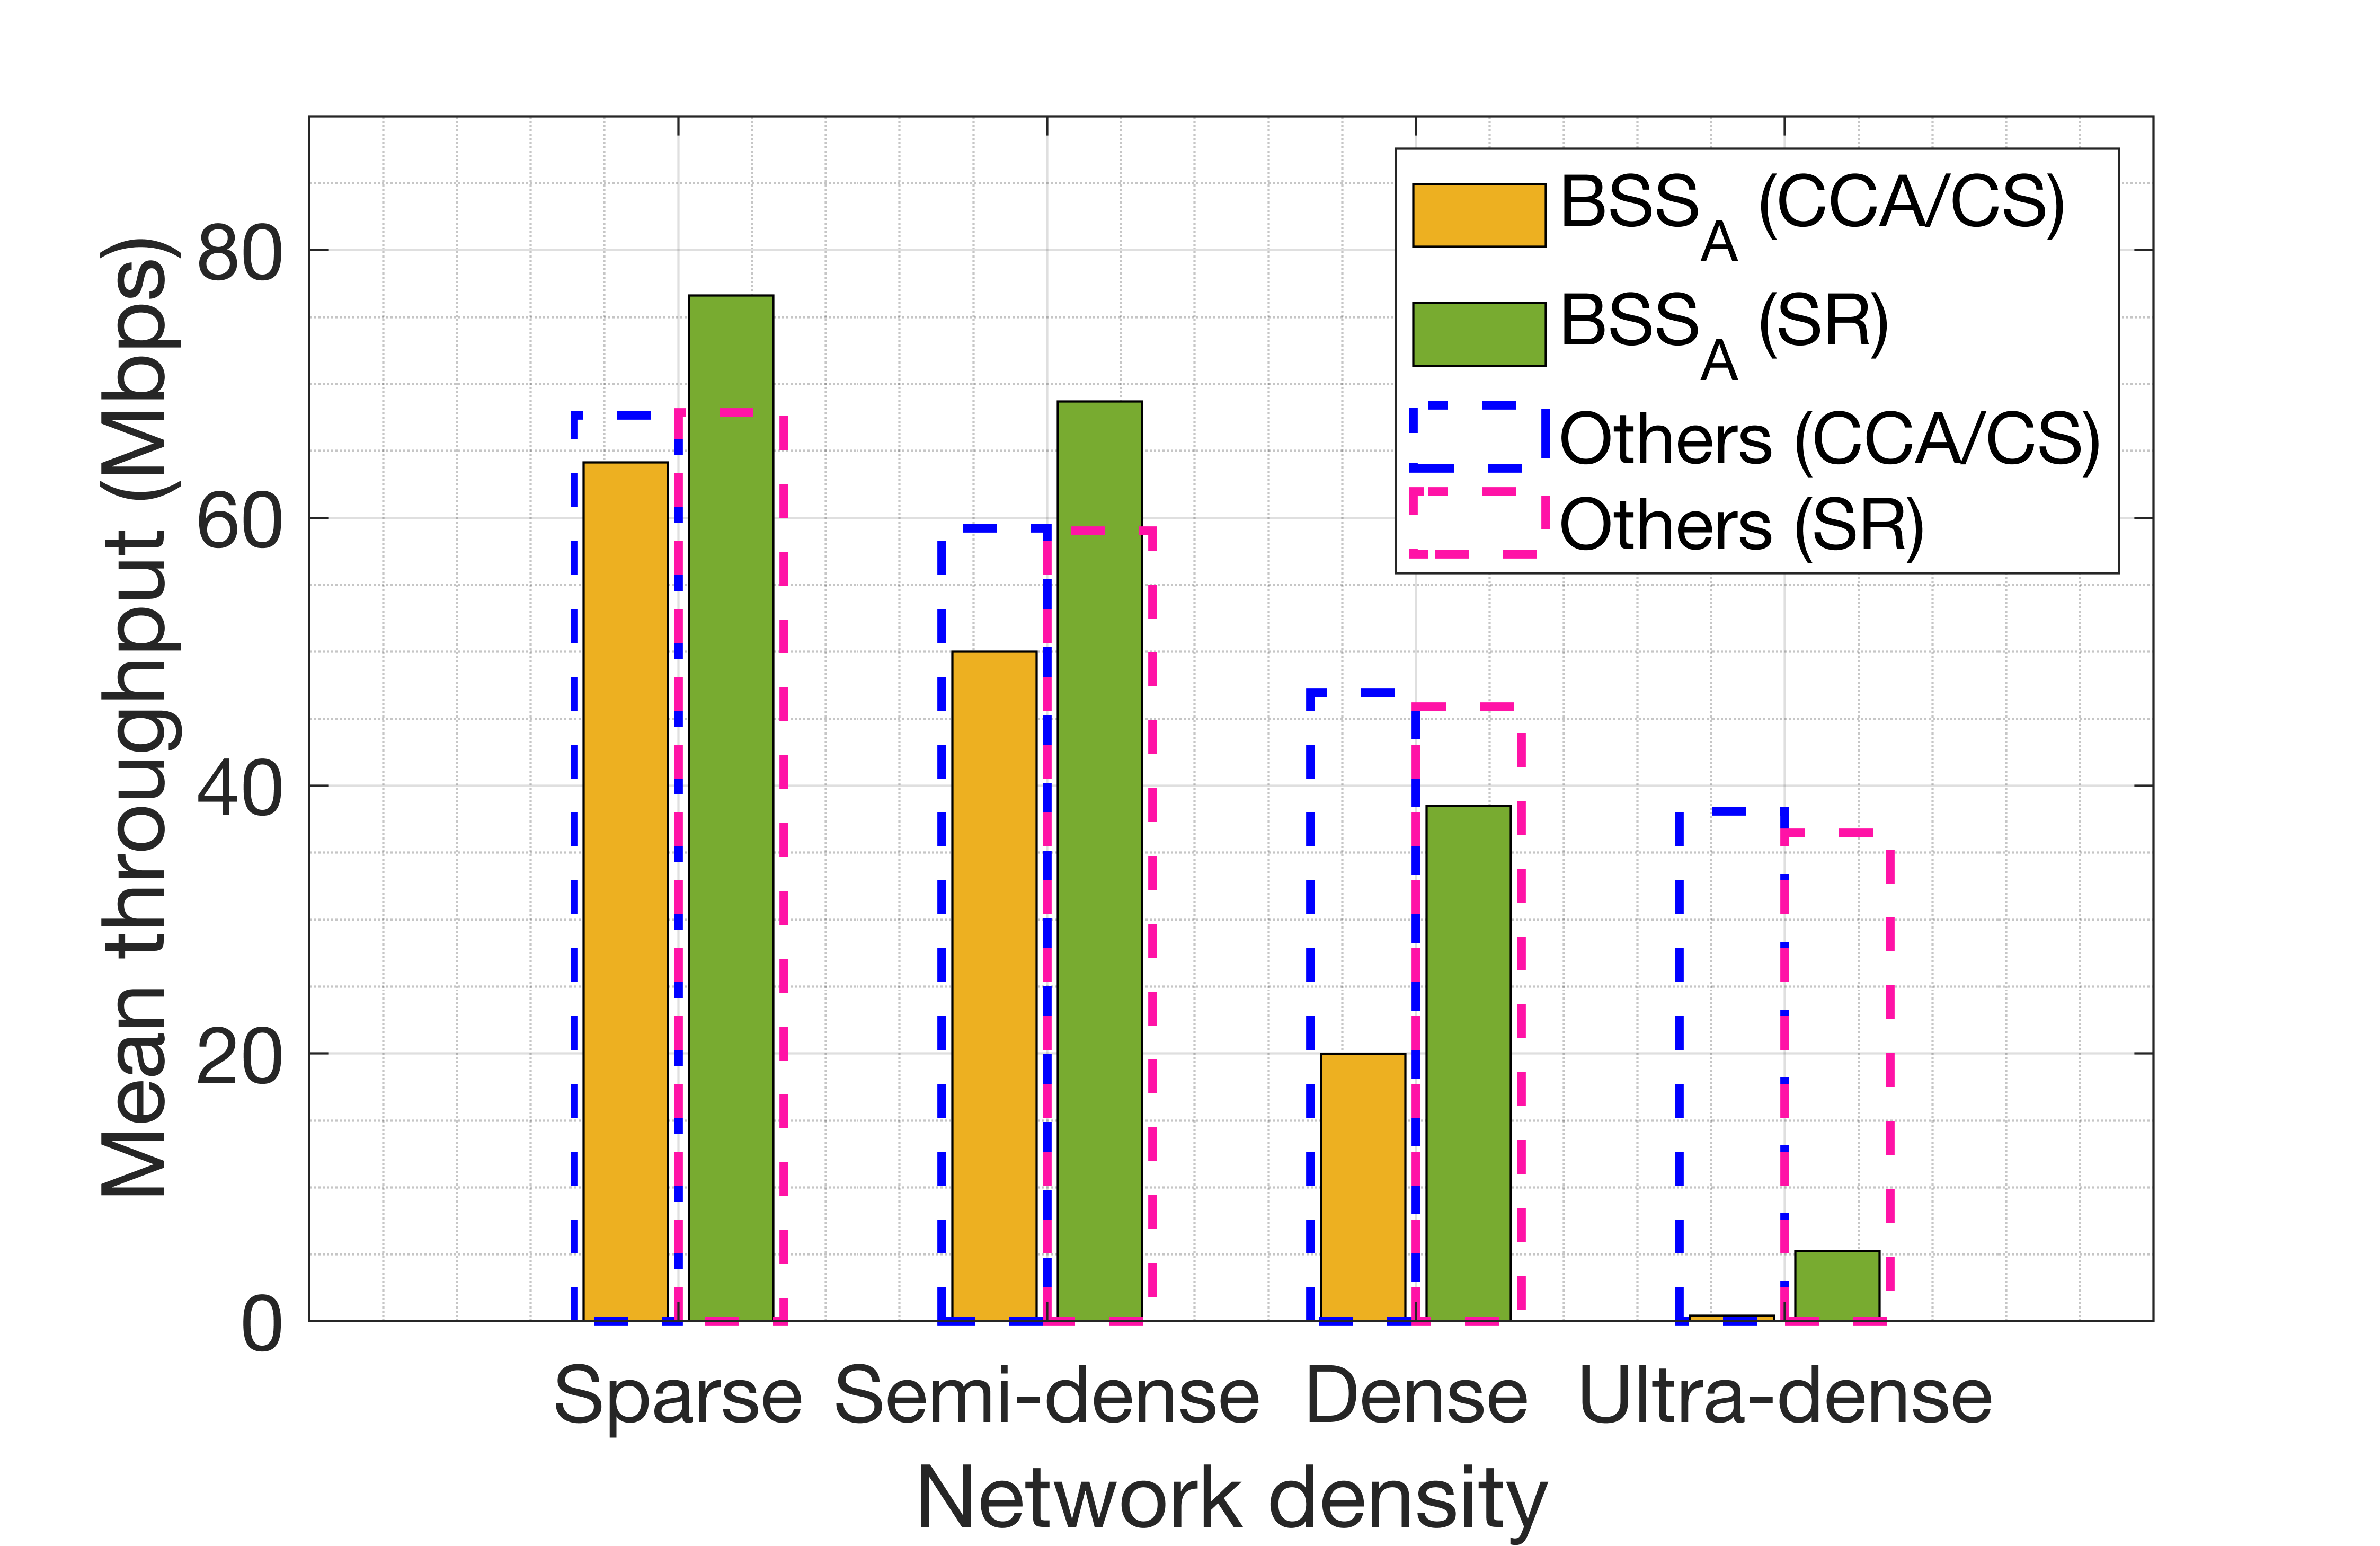
\includegraphics[width=.6\textwidth]{SIM_2_1}
	\caption{Mean throughput achieved with and without applying the SR operation in $\text{BSS}_A$, for each network density. Results show the mean throughput achieved by $\text{BSS}_A$ and the rest of BSSs.}
	\label{fig:SIM_2_1}
\end{figure}

First of all, if we focus on the throughput that $\text{BSS}_A$ experiences by default (amber solid bars), we notice a dramatic decrease as network density increases. Nevertheless, the SR operation allows $\text{BSS}_A$ to significantly improve the throughput (displayed by the green solid bars). Note, as well, that the maximum improvement is experienced at the dense scenario ($15\times15$ m). While the default performance is quite high for sparser scenarios, channel reutilization cannot be further improved at the ultra-dense scenario due to the high level of inter-BSS interference.

Apart from that, we observe that the average performance of the other BSSs (dashed bars) does not suffer radical changes for any of the network densities when $\text{BSS}_A$ applies SR. This is a really positive result, which indicates that SR allows improving the individual performance without affecting the rest of devices that do not apply the operation.

%%% TRAFFIC LOAD
\subsection{Traffic load}
\label{section:random_scenarios_traffic_load}
Besides network density, traffic load is another interesting factor to be studied with regards to the SR operation. To that purpose, we focus on the second densest scenario, which has been previously shown to achieve the maximum gains of the SR operation. In particular, we provide three different traffic loads ($l$), which are the same for all the BSSs: \emph{i)} low (1,000 packets/s, i.e., 12 Mbps), \emph{ii)} medium (2,000 packets/s, i.e., 24 Mbps), and \emph{iii)} high (10,000 packets/s, i.e., 120 Mbps). The traffic type considered is UDP in the downlink, which follows a Poisson distribution with $\lambda$ equal to the traffic load considered in each case.

Fig. \ref{fig:SIM_2_2} compares the performance achieved by default and SR configurations, for the different considered traffic load values. As done before, the results show the individual performance of $\text{BSS}_A$ and the average performance of the rest of BSSs. In particular, Fig. \ref{fig:SIM_2_2_2} shows the maximum improvements achieved by BSS$_A$ in terms of throughput. Notice that the SR configuration considers the OBSS/PD values that maximize BSS$_A$'s throughput. Based on that configuration, Fig. \ref{fig:SIM_2_2_1} shows the average channel occupancy (in \%).

\begin{figure}[ht!]
	\centering		
	%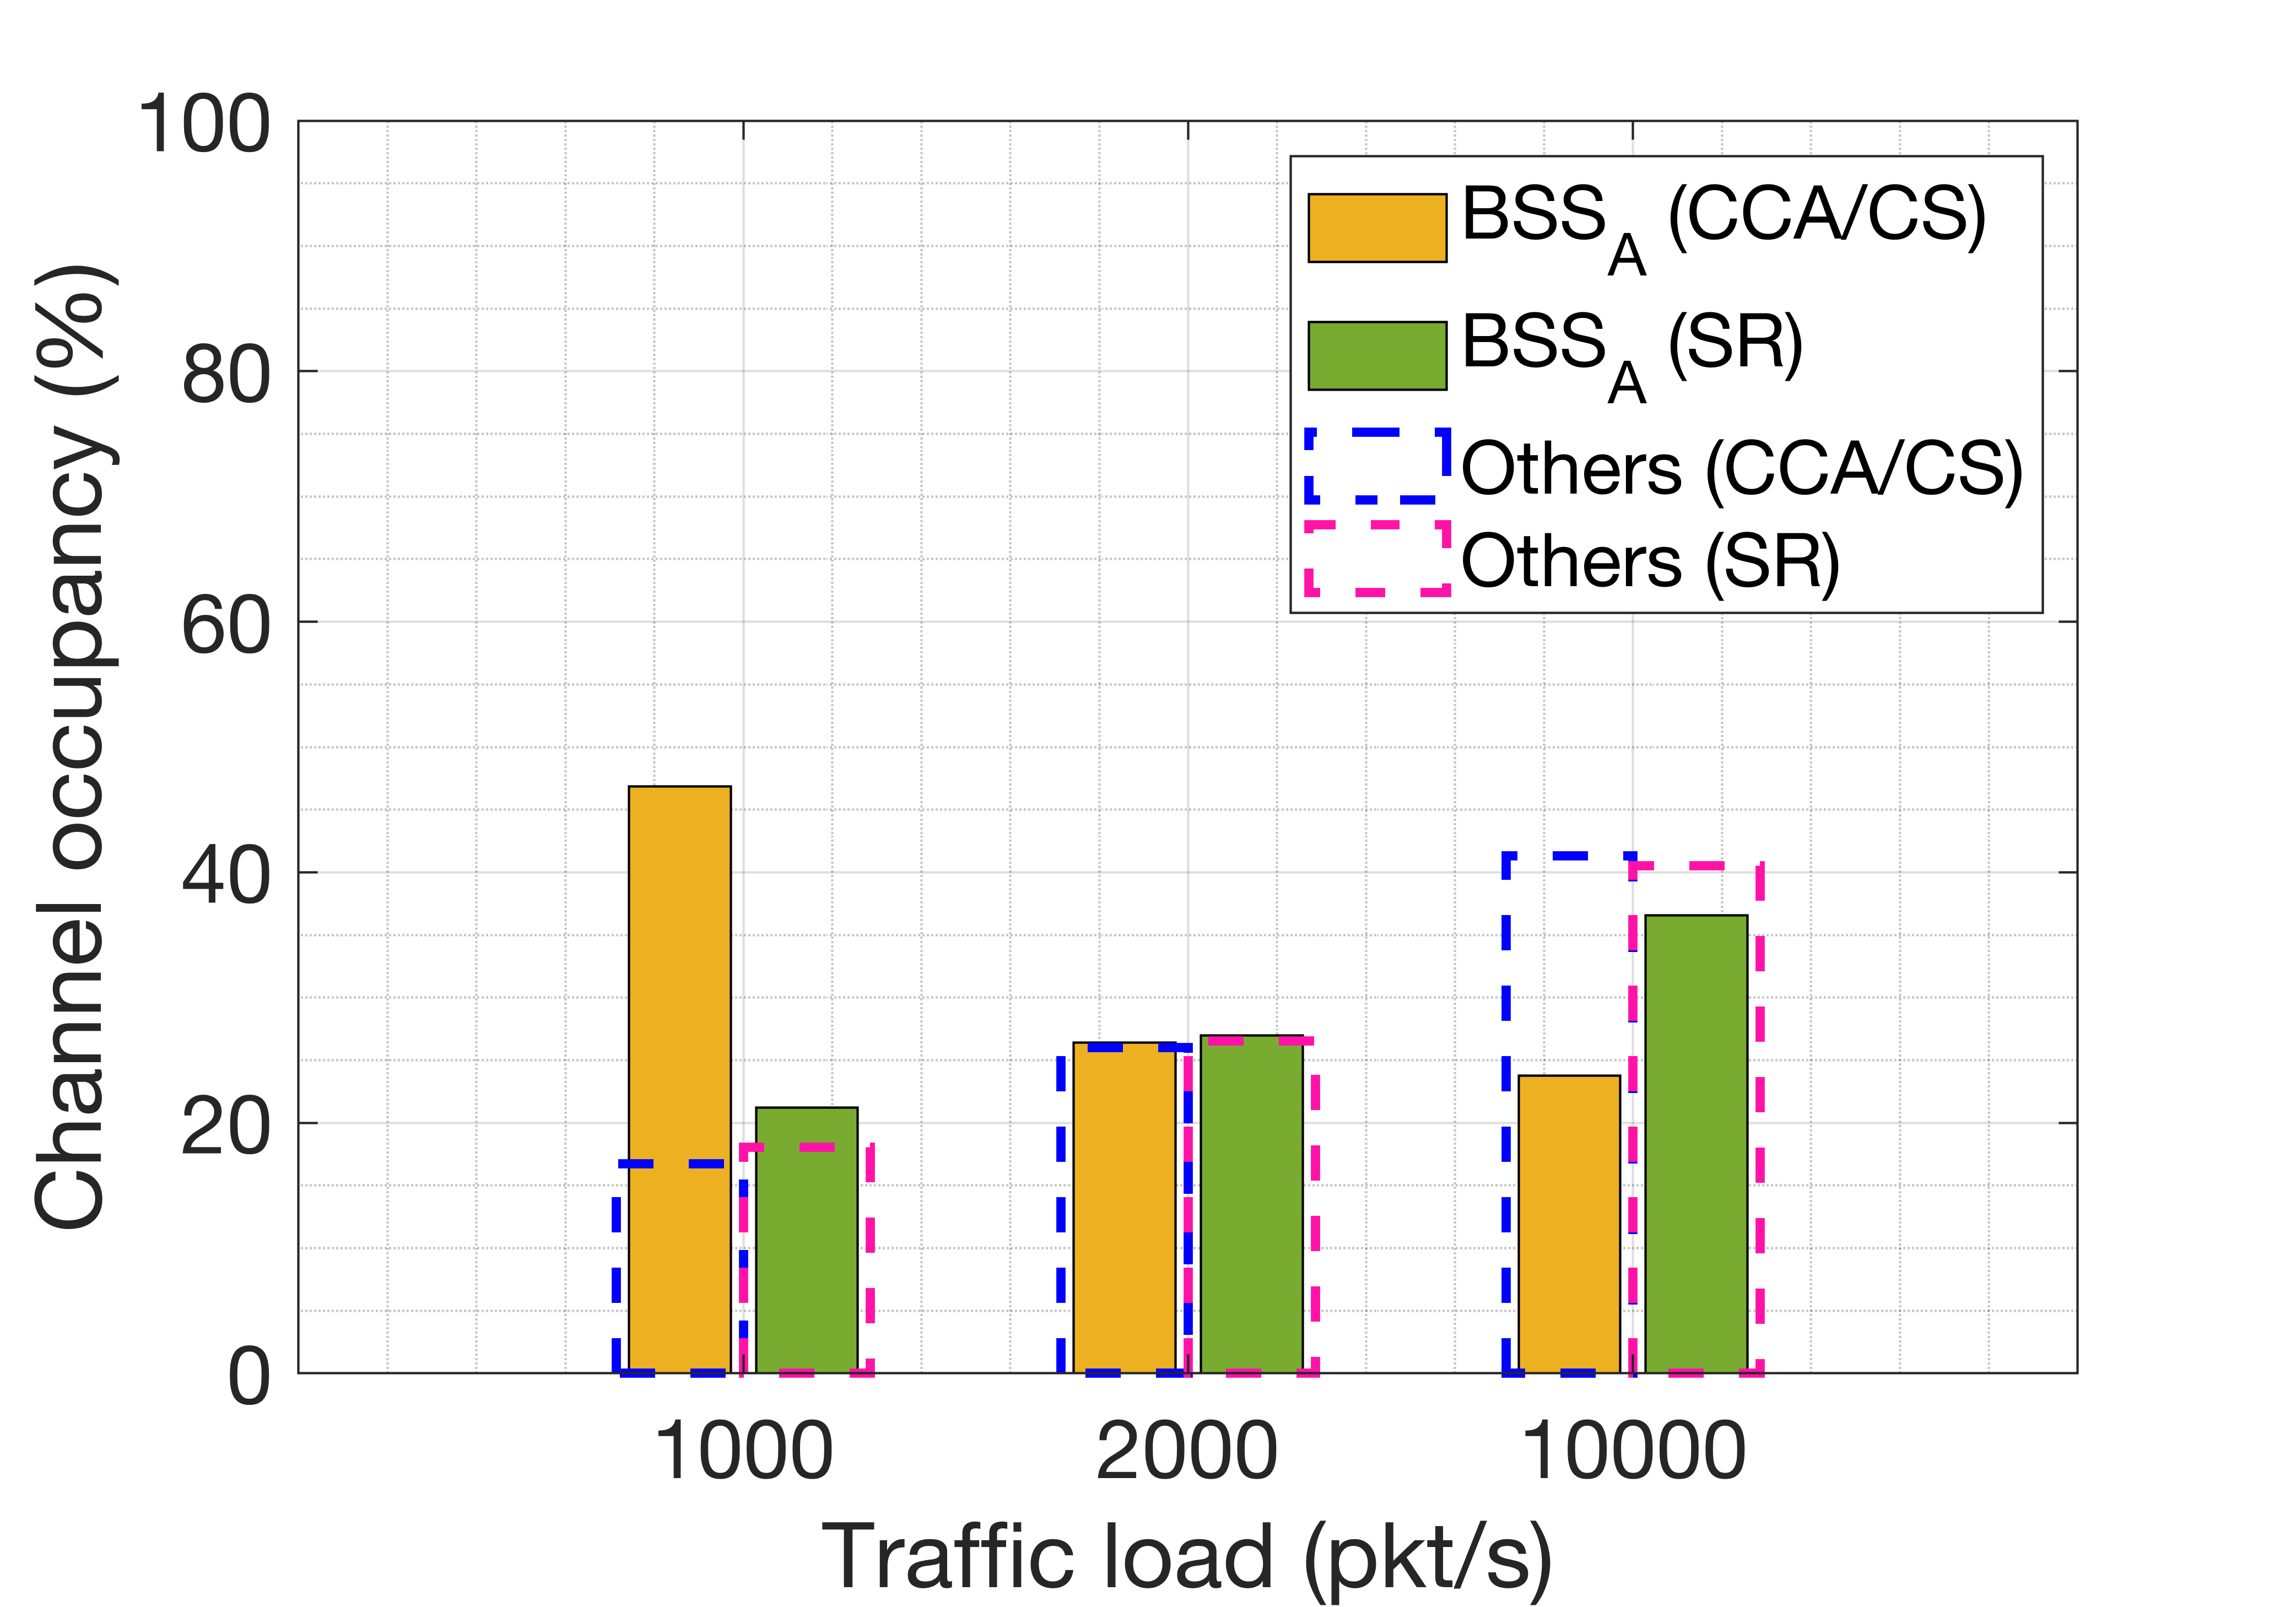
\includegraphics[width=\columnwidth]{SIM_2_2_1}
	\subfigure[Throughput]{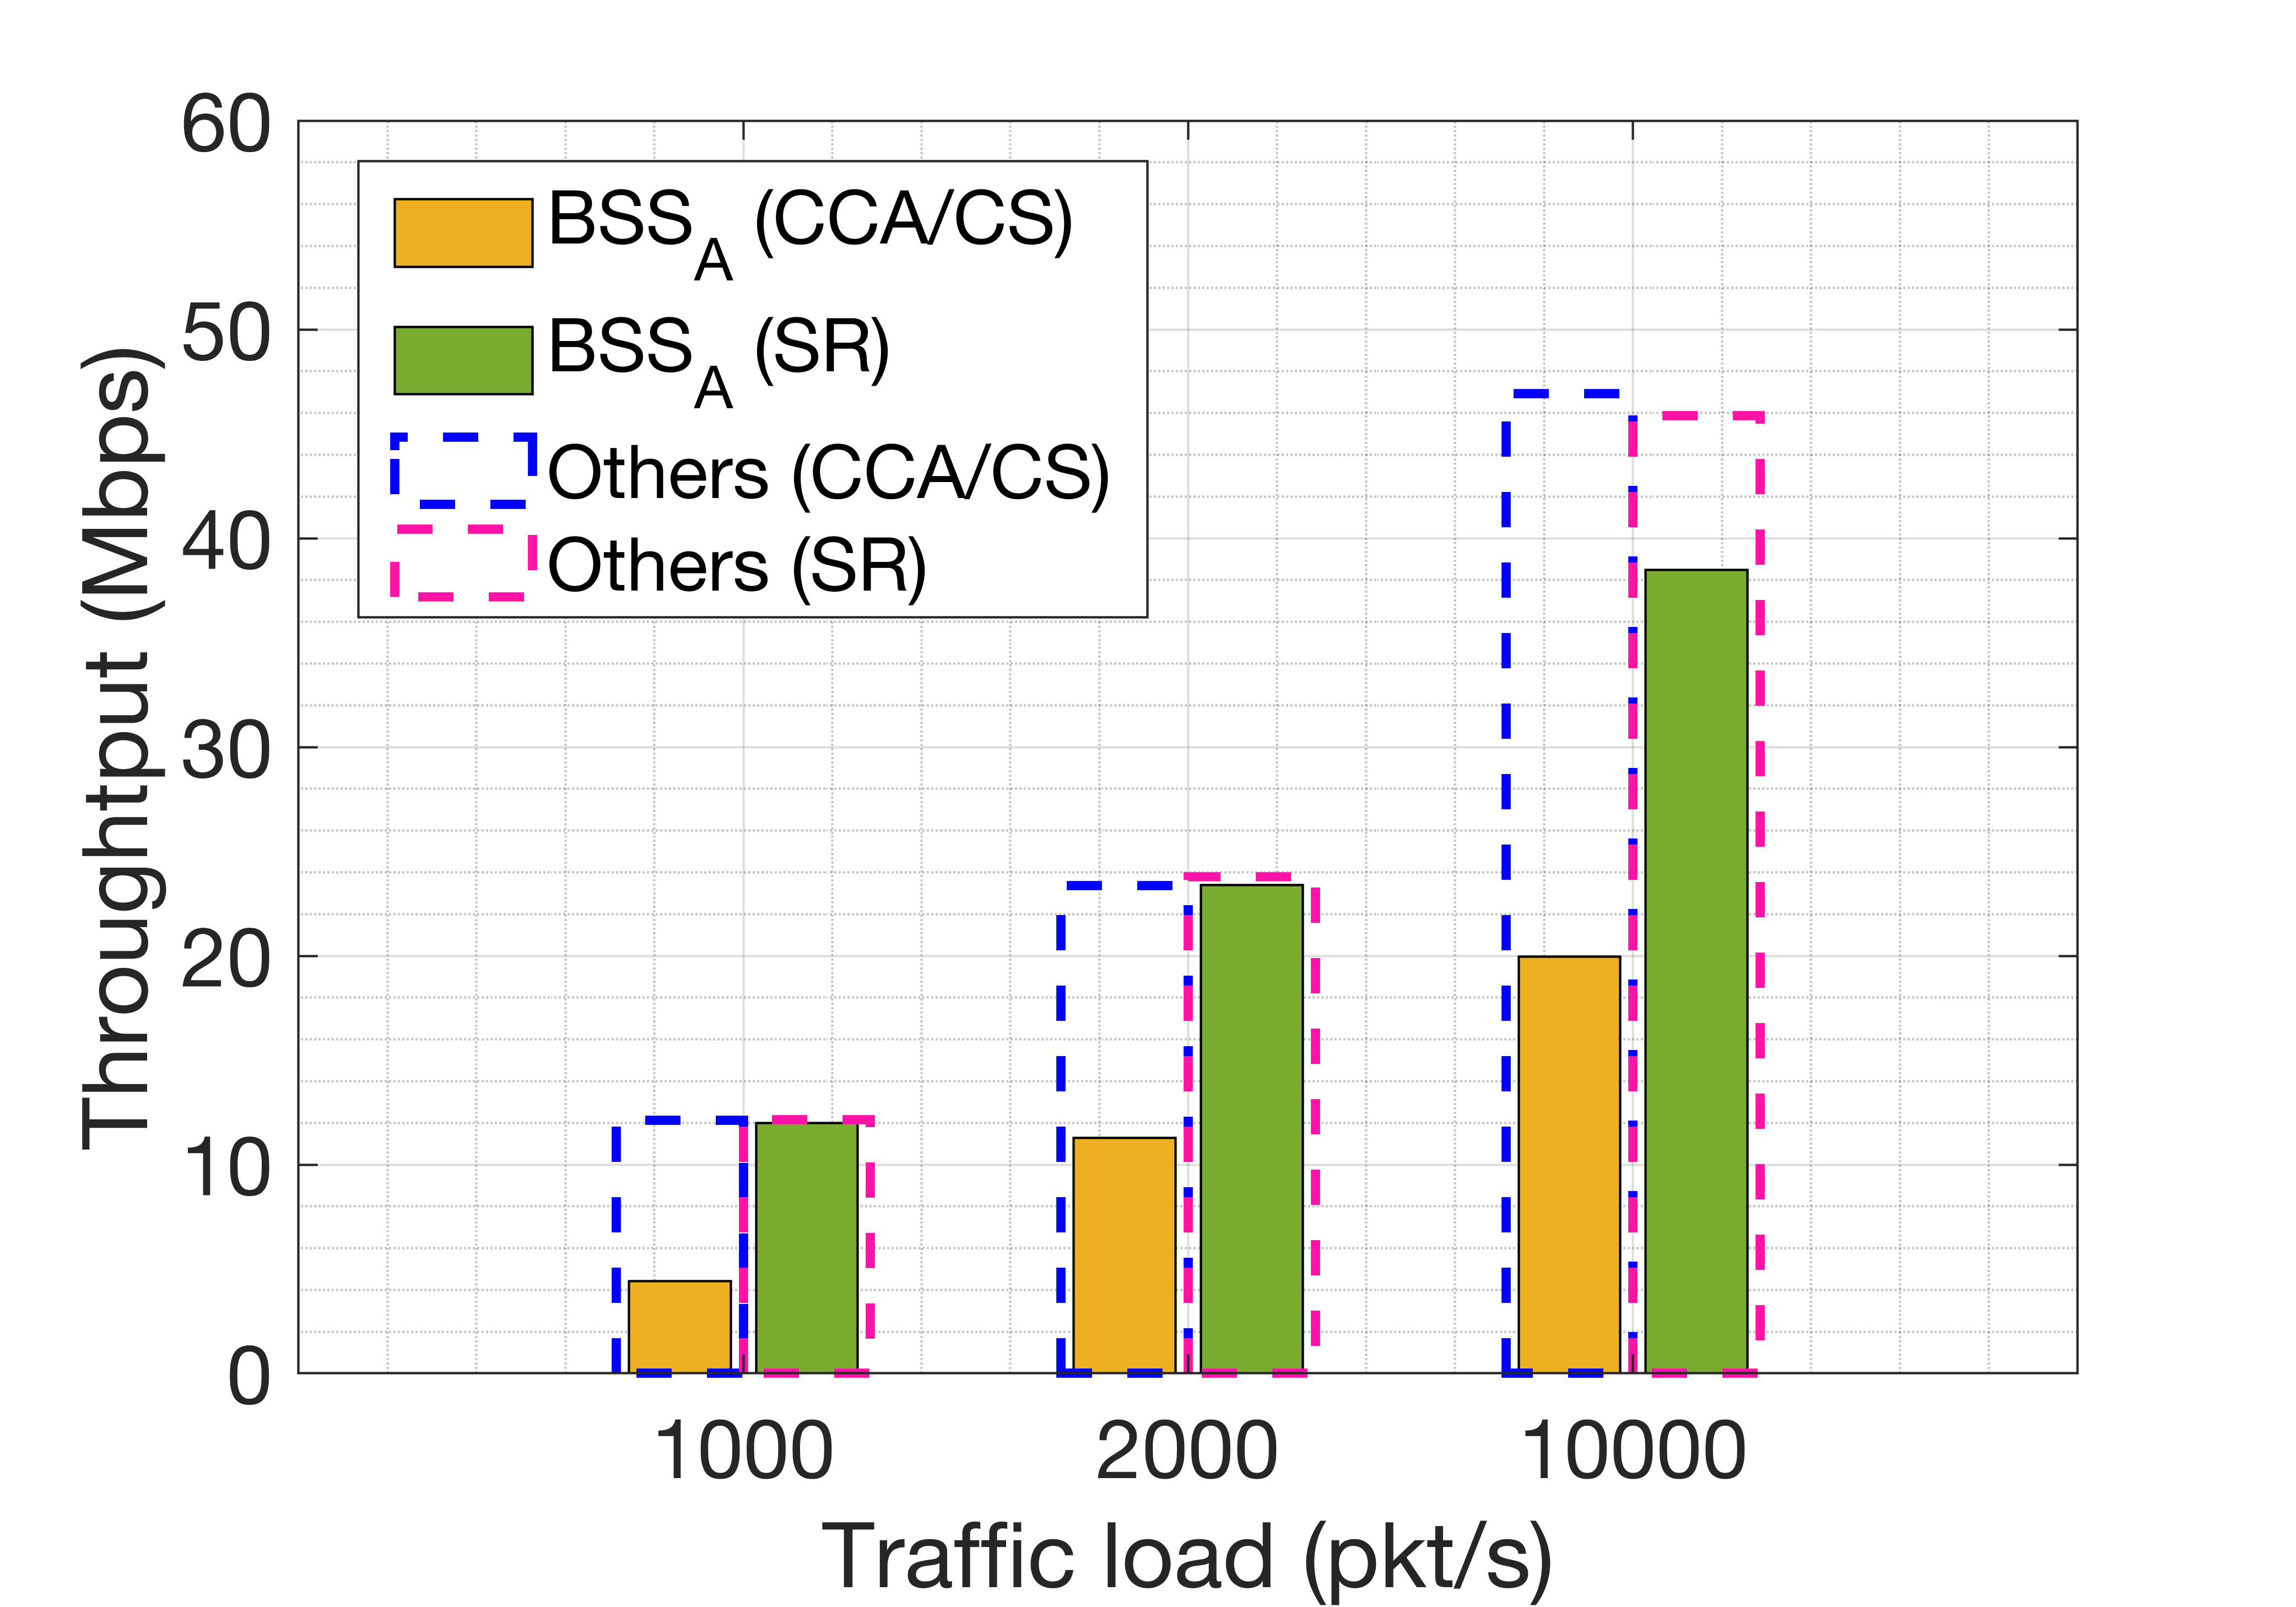
\includegraphics[width=.6\textwidth]{SIM_2_2_2}\label{fig:SIM_2_2_2}}%
	\subfigure[Channel occupancy]{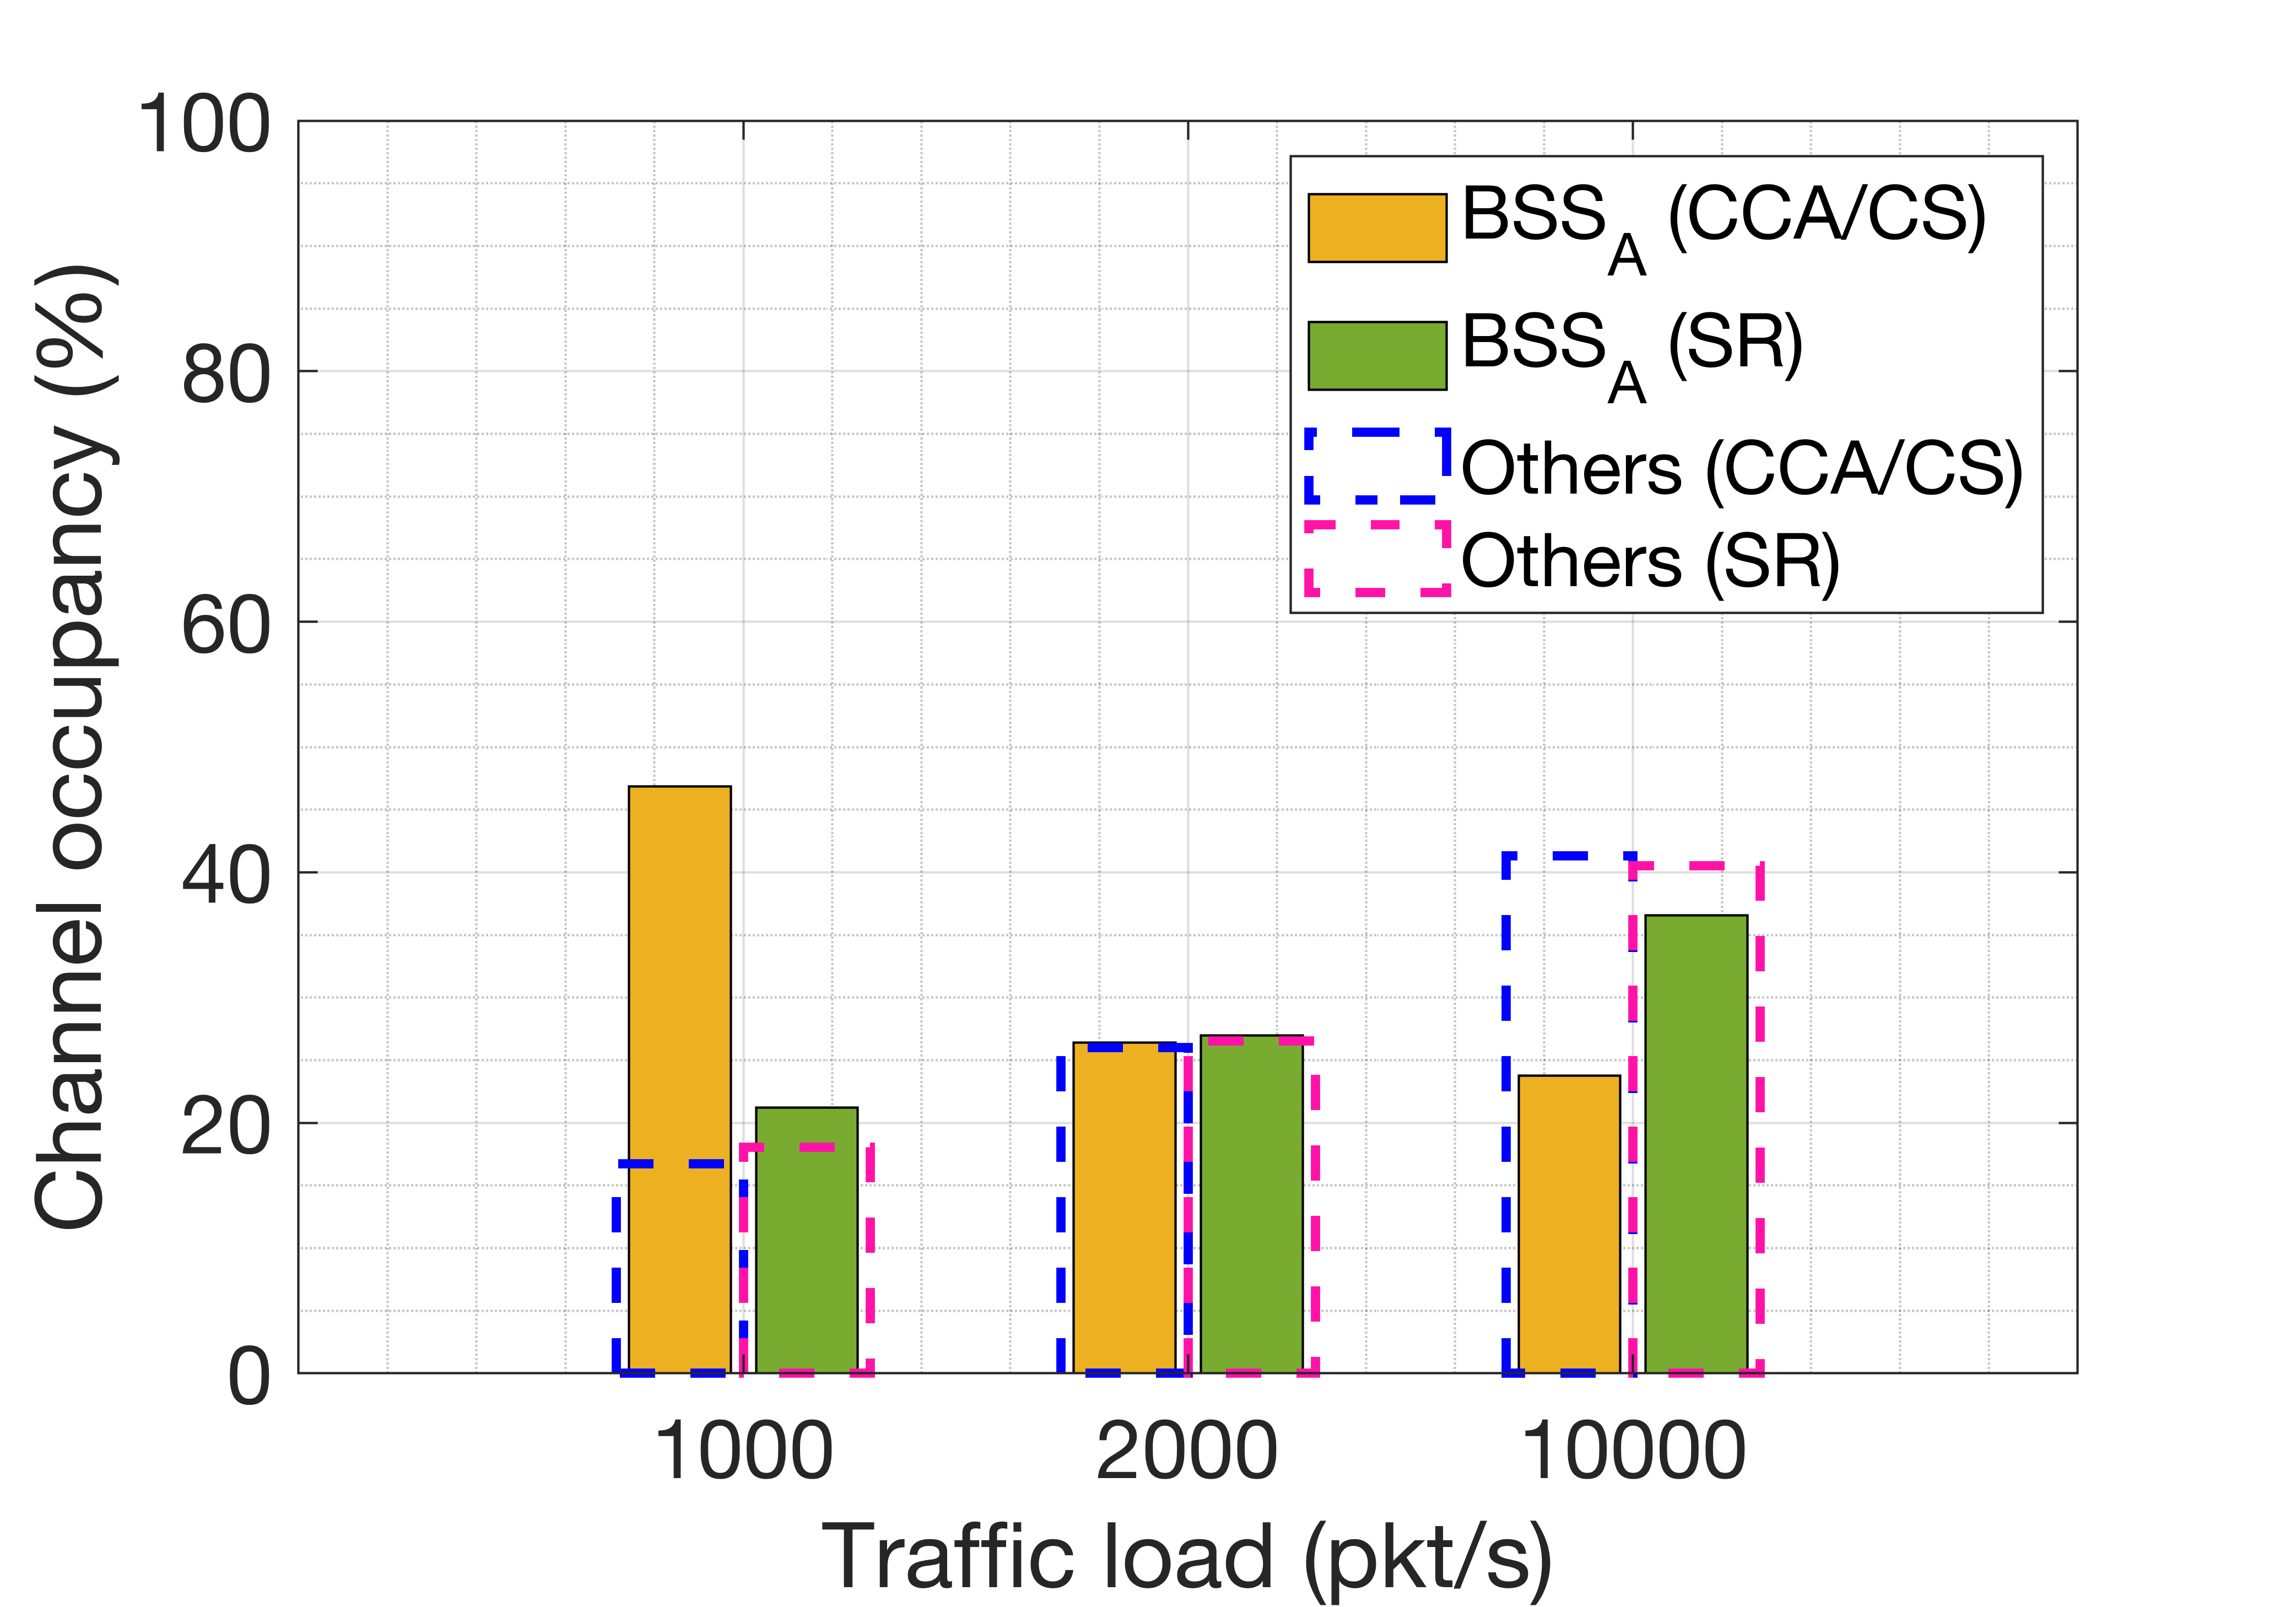
\includegraphics[width=.6\textwidth]{SIM_2_2_1}\label{fig:SIM_2_2_1}}
	\caption{Mean throughput and channel occupancy achieved with and without applying the SR operation in $\text{BSS}_A$, for each traffic load. Results are shown for $\text{BSS}_A$ and for the rest of BSSs (others).}
	\label{fig:SIM_2_2}
\end{figure}

As shown in Fig. \ref{fig:SIM_2_2_2}, $\text{BSS}_A$ obtains higher throughput gains as the traffic load increases. In particular, the highest gain is noticed for the largest traffic load (10,000 packets/s), which entails a saturation regime. This is a quite remarkable result since the interference noticed by $\text{BSS}_A$ is much higher when all the surrounding devices are constantly transmitting due to their high traffic load. Regarding channel occupation (shown in Fig. \ref{fig:SIM_2_2_1}), an interesting phenomenon is observed for the lowest traffic load. The fact is that the legacy CCA/CS configuration provides a higher channel occupancy than the SR one. However, this is not translated into a higher throughput, due to the high number of experienced collisions. Notice that collisions entail a high number of re-transmissions, which cause the observed increase in the occupancy. Finally, it is worth pointing out that the performance of the other BSSs is not affected in case $\text{BSS}_A$ applies SR.

%%% COLLABORATIVE SR
\subsection{Joint Spatial Reuse Operation}
\label{section:random_scenarios_collaborative}
So far, we have studied the effects of applying SR at a single BSS (i.e., $\text{BSS}_A$). Now, we assess the potential of the joint operation by defining different situations based on the number of BSSs that apply SR. Provided that $\text{BSS}_A$ always applies the SR operation, we propose three study cases: 
\begin{itemize}
	\item \textbf{Legacy:} all the other BSSs employ the default CCA/CS.
	\item \textbf{Mixed SR:} at the beginning of the simulation, each BSS randomly decides (with same probability) whether to apply the SR operation or to remain using the default configuration.
	\item \textbf{All SR:} all the BSSs apply the SR operation. 
\end{itemize}

In order to compare the effects of applying SR in parallel with other BSSs, we define the following metrics: \emph{i)} throughput ($\Gamma$), \emph{ii)} percentage of time occupying the channel ($\rho$), and \emph{iii)} average delay for transmitting a packet once it arrives at the queue ($d$). For each metric, we consider the performance improvements achieved by $\text{BSS}_A$ (indicated with subindex \emph{A}), and the average across the rest of BSSs (indicated with subindex \emph{O}).

Fig. \ref{fig:SIM_2_3} shows the potential improvements achieved when applying SR in each of the proposed scenarios. While Fig. \ref{fig:SIM_2_3_1} shows the performance of BSS$_A$, Fig. \ref{fig:SIM_2_3_2} focuses on the performance of the others. For that purpose, the empirical cumulative distribution function (CDF) is used for each of the performance metrics. Notice that we have considered the densest scenario ($25\times25$m) and the highest traffic load (10,000 packets/s), thus representing the worst-case situation. As done before, we have generated 50 random scenarios for averaging purposes, and, for each of them, we have tried all the possible OBSS/PD values to be used homogeneously by the BSSs applying the SR operation. Accordingly, we have used the best value to extract the maximum average improvement of SR with respect to the legacy configuration. In every situation (\emph{legacy}, \emph{mixed} and \emph{all SR}), we select the best OBSS/PD threshold from $\text{BSS}_A$'s point of view, which is also used to assess its impact on the others. Again, the SR configuration used for the channel occupancy is the one whereby $\text{BSS}_A$'s throughput is maximized.

\begin{figure*}[ht!]
	\centering		
	\subfigure[BSS$_A$]{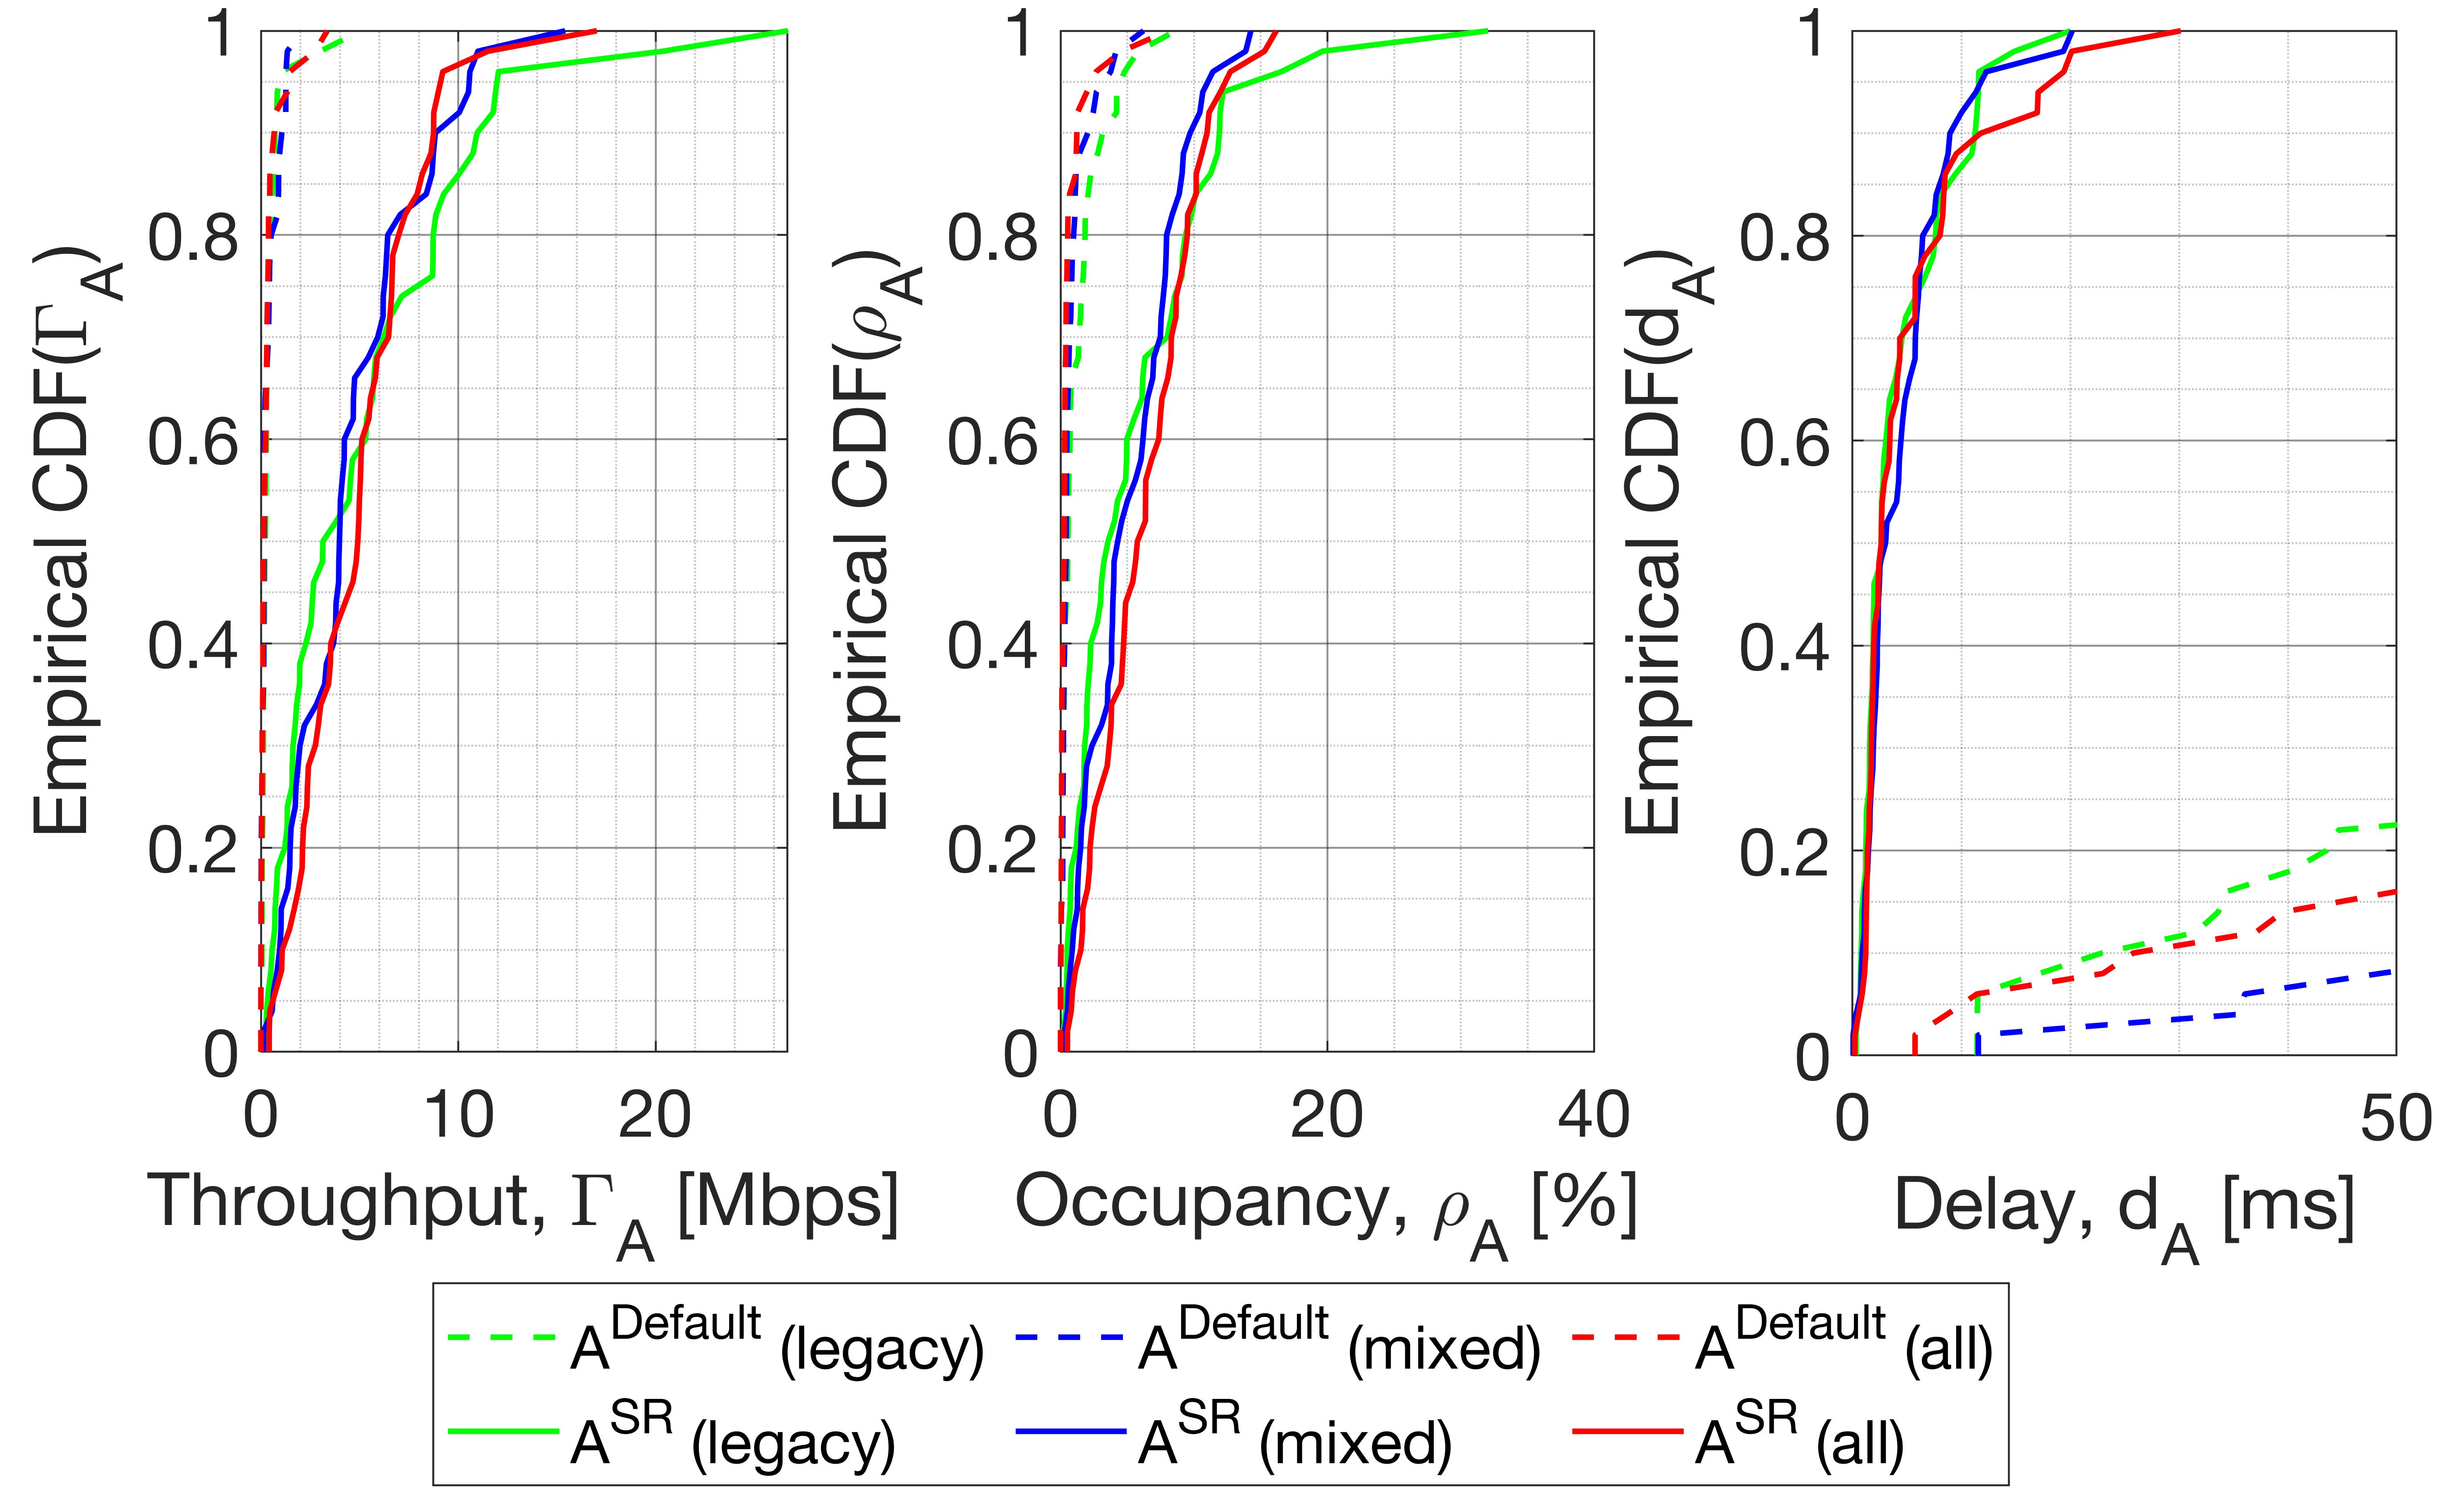
\includegraphics[width=.55\columnwidth]{SIM_2_3_1}\label{fig:SIM_2_3_1}}%
	\subfigure[Others]{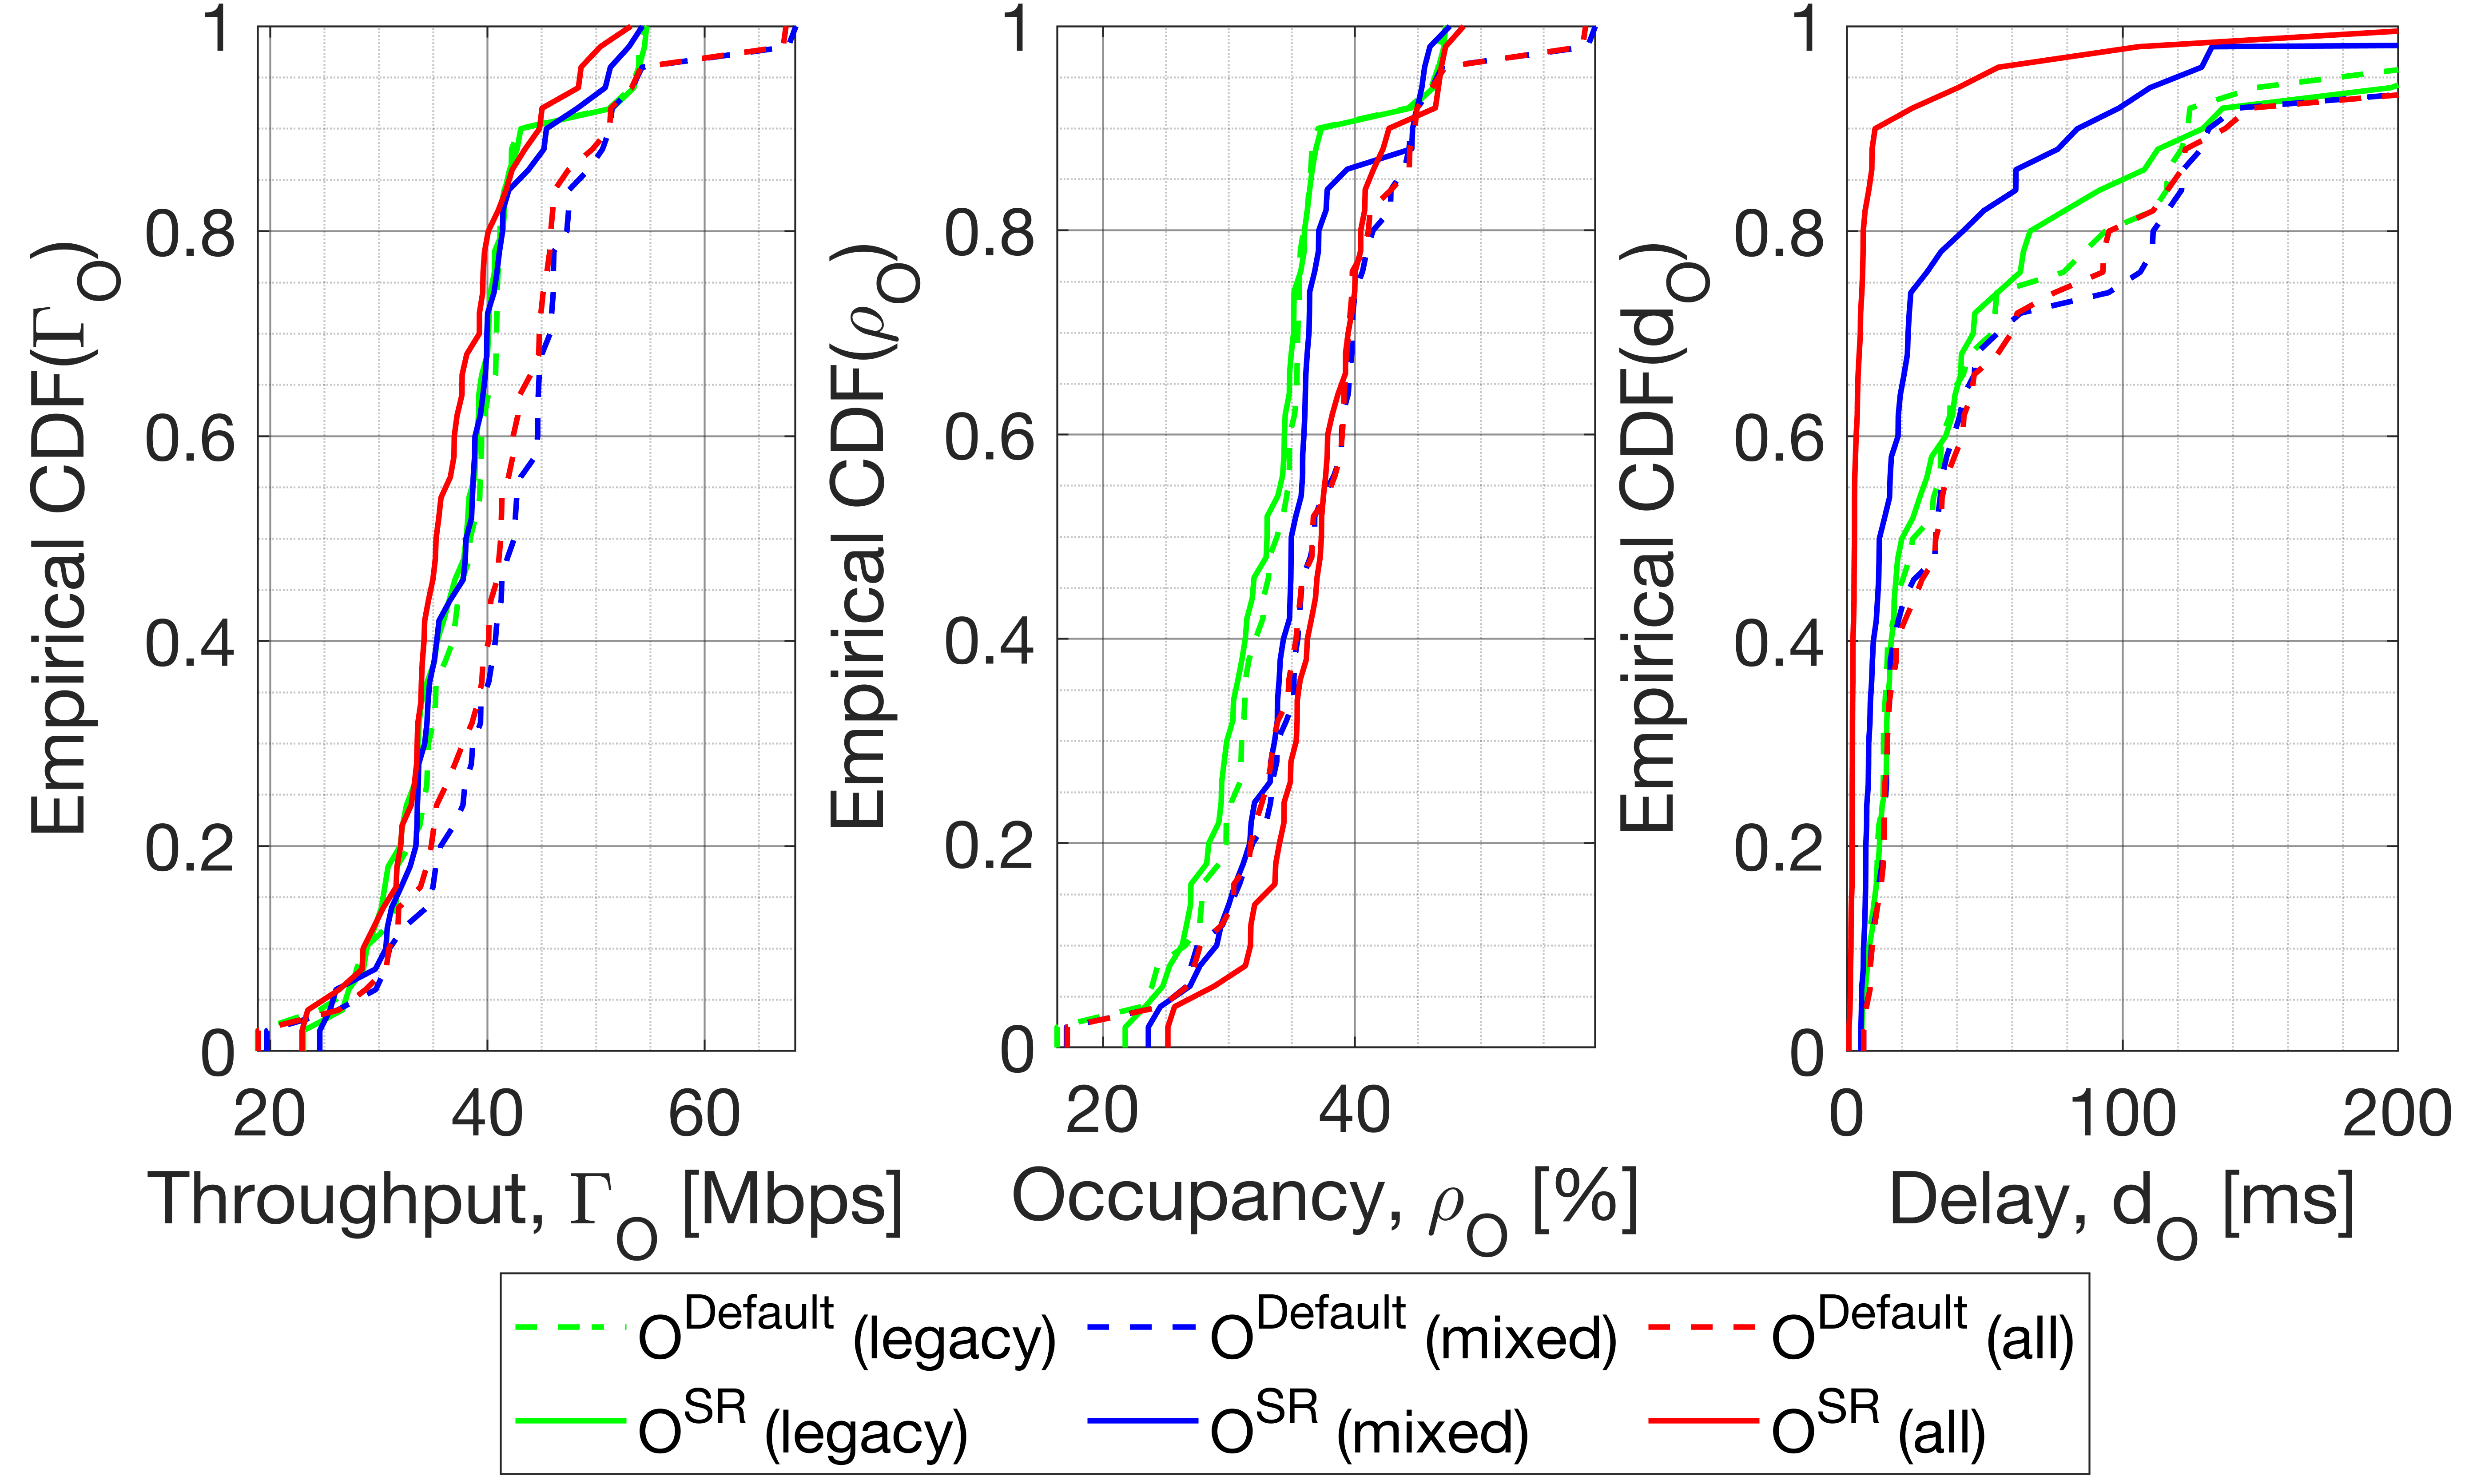
\includegraphics[width=.55\columnwidth]{SIM_2_3_2}\label{fig:SIM_2_3_2}}
	\caption{Mean performance improvements achieved for each SR setting by BSS$_A$ ($A$) and the others ($O$). The results are shown for the OBSS/PD values that maximize the performance of BSS$_A$.}\label{fig:SIM_2_3}
\end{figure*}

As shown in Fig. \ref{fig:SIM_2_3_1}, $\text{BSS}_A$ achieves similar performance improvements, regardless of whether the environment applies SR or not. In particular, a high gain is noticed on the average delay. Moreover, regarding the others' performance (Fig. \ref{fig:SIM_2_3_2}), a null improvement is observed on the throughput, even for the \emph{all SR} context. In contrast, the delay is notably reduced as the number of BSSs using SR increases.

% ----------------------------------
% -
% 	-- Gaps --
% -
% ----------------------------------
\section{Ways Forward and Research Opportunities}
\label{section:ways_forwad}
The IEEE 802.11ax SR operation can potentially increase spectral efficiency in dense deployments. However, it is already in a premature stage and further developments are expected to sustain progress towards next-generation wireless deployments. 

\subsection{Unexplored Areas within the Spatial Reuse Operation}
In the context of the SR operation, the following areas have not been fully exploited yet:
\begin{itemize}
	\item \textbf{Assignment of BSS colors:} as discussed in Sections \ref{section:bss_coloring} and \ref{section:obss_pd_based}, BSS coloring is key for the OBSS/PD-based SR operation since it allows differentiating between intra and inter-BSS frames. However, the way BSS colors are assigned to BSSs is not specified, thus leading to potential collisions and miss-behaviors regarding the SR operation.
	\item \textbf{Election of SRGs:} similarly to the BSS color, the SRG is used to sub-classify inter-BSS frames, so that different PD policies can be applied to increase spectral efficiency. However, forming SRGs is not trivial since inter-BSS interactions must be carefully captured to properly taking advantage of the SR operation. The set of policies regarding SRGs may be decided by the APs, as a result of monitoring phases.% (e.g., after experiencing several packet losses).
	\item \textbf{Establishment of OBSS/PD thresholds:} the election of OBSS/PD thresholds for each type of frame (SRG, and non-SRG) entails a set of trade-offs. On the one hand, too low values may lead to null improvement, thus framing the legacy operation whereby the channel is shared. On the other hand, too high values may generate performance anomalies such as the hidden-terminal problem or flow starvation. A potential solution to properly establish each OBSS/PD threshold is to capture all the inter-BSS interactions on a per-STA basis.
	\item \textbf{Optimal transmit power:} the current transmit power restriction is useful to prevent the accentuation of unfair situations. However, the performance of the SR operation may be further increased in case of properly leveraging the transmit power according to the noticed interactions among nodes.
	\item \textbf{Disabling the SR operation:} there are situations in which the SR operation may be harmful to certain devices (e.g., in terms of fairness). Therefore, a given BSS must be able to identify whether the SR operation must be disabled or not. This can be achieved by setting the OBSS/PD threshold to the default CCA/CS value. Alternatively, the SR operation can be disabled at STAs only, thus leading to an AP-only SR setting. In this regard, AP-AP interactions would be mostly targeted.
\end{itemize}

Solving most of the aforementioned problems is not straightforward and requires an in-depth analysis to offer optimal or close-to-optimal solutions. While BSS color assignment may appear to be straightforward (e.g., through graph coloring techniques), defining OBSS/PD thresholds is a very complex task that embraces many variables. In particular, inter-BSS interactions have been shown in this paper to significantly vary depending on the selected OBSS/PD values. Since the performance of IEEE 802.11 BSSs is not linear with the sensitivity and the transmission power (due to the nature of CSMA/CA), the optimal OBSS/PD threshold cannot be computed explicitly. Notice that the number of total combinations in an N-BSS scenario is $C = 21^\text{N}$, for 21 different non-SRG OBSS/PD thresholds. Therefore, the problem is intractable. If considering SRGs, the problem becomes even more complex since the number of combinations is $C = (21\times21)^\text{N}$ (provided that we have 21 values to be used for SRG and non-SRG OBSS/PD thresholds).

\subsection{Integration of the Spatial Reuse Operation with other Techniques}

% Other ways forward
In addition to problems specific to the SR operation, the integration with many other novel mechanisms remains unexplored. Among them, we highlight OFDMA \cite{bankov2018ofdma, dovelos2018optimal}, multiple antenna systems \cite{liao2016mu}, and scheduled transmissions \cite{nurchis2019target}. The potential of SR goes further when combined with other techniques. 

For instance, the combination of SR with directional transmissions may lead to efficient and performance maximizing communications, where SR is applied on a per-beam basis. Fig. \ref{fig:sr_and_beamforming} devises the potential of combining SR with directional transmissions. As illustrated, $\text{BSS}_A$ applies the SR operation on a per-beam basis, while $\text{BSS}_B$ remains using the default CCA/CS. In particular, collisions by hidden-node may be experienced for $\text{STA}_\text{A3}$, in case of using the inter-BSS OBSS/PD. However, channel reuse can be enhanced for transmissions to $\text{STA}_\text{A1}$ and $\text{STA}_\text{A2}$, which are out of range of $\text{AP}_B$. Therefore, the inter-BSS OBSS/PD can be used only for transmissions involving those two STAs, while a more conservative threshold can be employed for $\text{STA}_\text{A3}$.

\begin{figure}[ht!]
	\centering		
	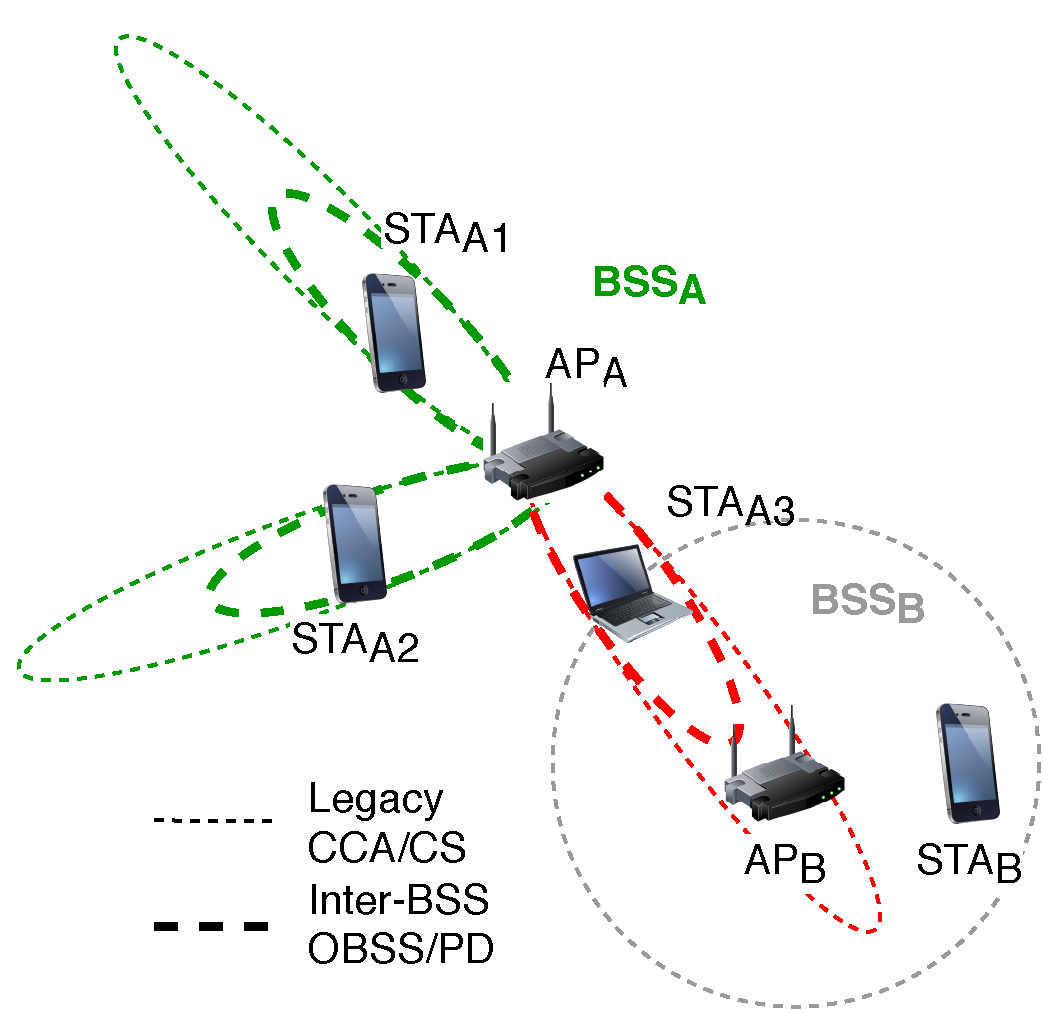
\includegraphics[width=0.5\textwidth]{sr_and_beamforming}
	\caption{Potential application of SR combined with directional transmissions.}
	\label{fig:sr_and_beamforming}
\end{figure}

\begin{figure*}[ht!]
	\centering		
	\subfigure[Scenario]{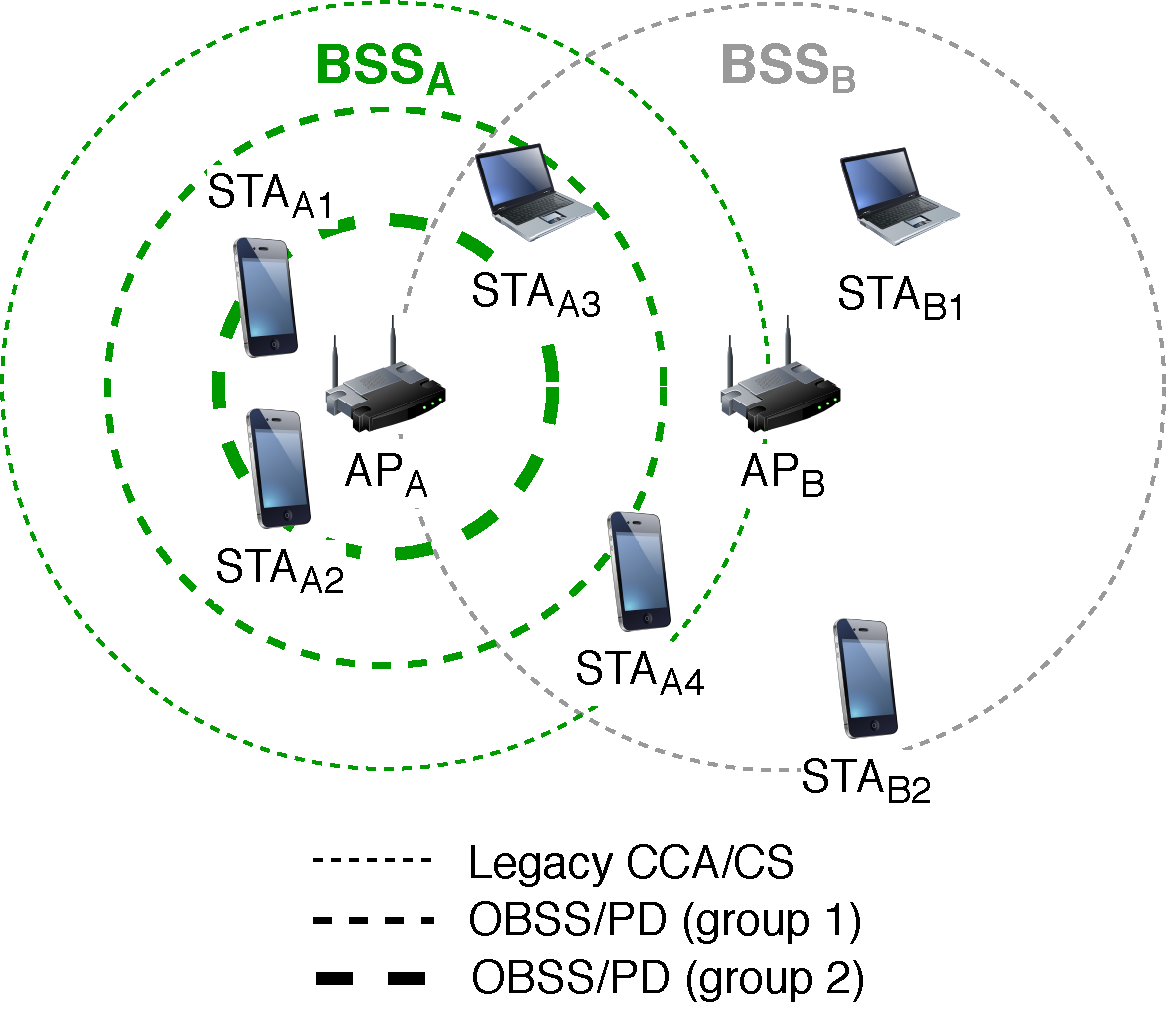
\includegraphics[width=0.4\textwidth]{sr_and_tb}\label{fig:sr_and_tb_a}}
	\subfigure[Packets exchange]{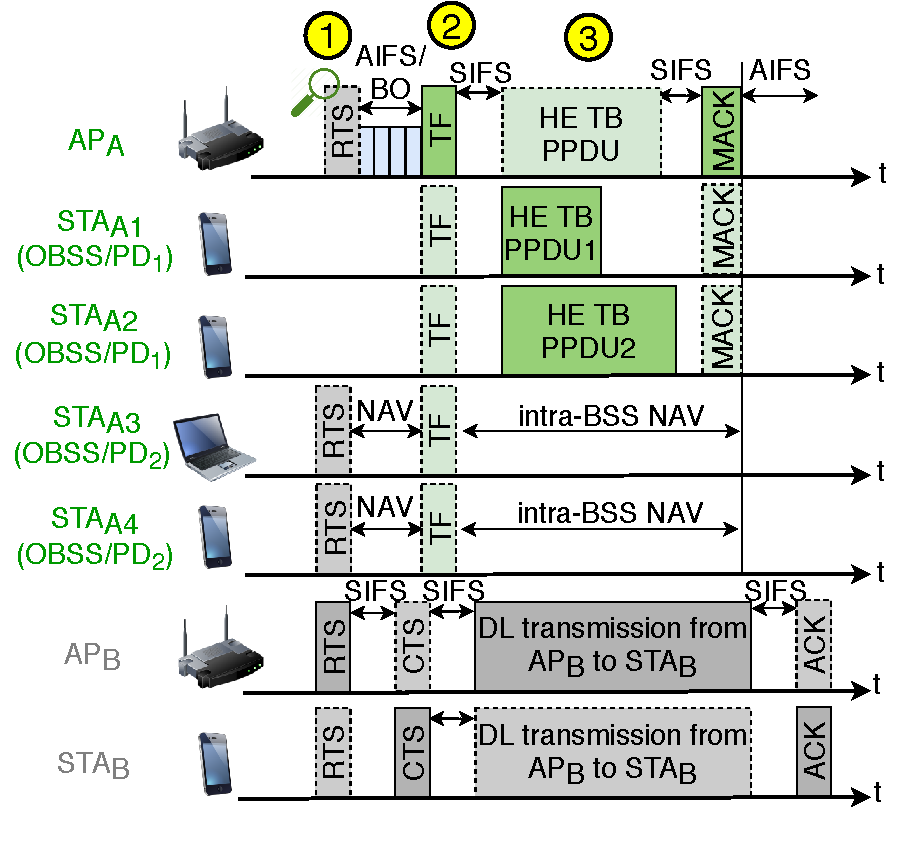
\includegraphics[width=.45\columnwidth]{sr_and_tb_b}\label{fig:sr_and_tb_b}}
	\caption{Potential application of SR combined with TB communications.}		
	\label{fig:sr_and_tb}
\end{figure*}

Similarly to the integration with directional antennas, the potential of SR can be further exploited through TB communications. In this case, users of a given BSS can be categorized into different types, so that different inter-BSS OBSS/PD values are assigned to them. Figure \ref{fig:sr_and_tb_a} shows how users can be grouped based on different OBSS/PD thresholds. As a result, transmissions within the same BSS can be scheduled in a differently, thus improving spectral efficiency. In the proposed example, $\text{STA}_\text{A1}$ and $\text{STA}_\text{A2}$ belong to the first group because of their privileged position with respect to $\text{AP}_A$. Therefore, a more aggressive OBSS/PD threshold is employed at the time of scheduling transmissions to these stations. The same reasoning can be applied to $\text{STA}_\text{A3}$, which, in this case, requires the usage of a more conservative OBSS/PD threshold for being scheduled in combination with SR. Finally, the legacy CCA/CS is used for $\text{STA}_\text{A4}$, in order to prevent negative interactions with respect to $\text{BSS}_B$. It is worth pointing out that users belonging to different groups can be scheduled together, provided that the most restrictive OBSS/PD threshold is used. 

In Fig. \ref{fig:sr_and_tb_b}, we show a data transmission resulting from the combination of TB communications and SR. In the yellow point \#1, $\text{AP}_A$ detects an inter-BSS transmission from $\text{AP}_B$, which can be ignored by using the most aggressive OBSS/PD, i.e., the one devoted for STAs in group 1. Accordingly, it schedules an uplink transmission from $\text{STA}_\text{A1}$ and $\text{STA}_\text{A2}$ (yellow point \#2). Finally, $\text{AP}_A$ receives the scheduled transmissions from group 1 (yellow point \#3).

\subsection{Artificial Intelligence to Address Spatial Reuse Optimization}
In light of the challenges posed by the 11ax SR operation, Artificial Intelligence (AI) emerges as a potential solution. In particular, WLANs are characterized by being highly varying in terms of users and channel dynamics. Moreover, we typically find decentralized deployments, at which none or little coordination is allowed. Hence, online learning stands as a suitable technique to address the optimization of SR in WLANs. In fact, many works on OBSS/PD adjustment, such as DSC \cite{smith2015dynamic} and COST \cite{selinis2018control}, are based on iterative methods. 

Machine Learning (ML), and more precisely Reinforcement Learning (RL), can contribute to improving the performance of the already existing methods. RL has been shown to properly fit with the decentralized nature of IEEE 802.11 WLANs \cite{long2007non, naddafzadeh2010distributed, zhou2011reinforcement, ghadimi2017reinforcement, wilhelmi2019collaborative, wilhelmi2019potential}. In particular, the usage of RL allows capturing subtle information that cannot be predicted before-hand (for instance, regarding inter-BSS interactions). Such information enables conducting a learning-based procedure, which is aimed at increasing performance while reducing the number of undesired situations (e.g., poor fairness).

% ----------------------------------
% -
% 	-- Conclusions --
% -
% ----------------------------------
\section{Conclusions}
\label{section:conclusions}
In this paper, we have provided an extensive tutorial of the IEEE 802.11ax SR operation, which aims to maximize the performance of next-generation WLANs by increasing the number of parallel transmissions. Our purpose has been to do so in a clear and easy-to-understand manner. Thus, significant efforts have been made in providing meaningful examples of the different specifications related to SR. %First of all, we have presented the concepts that enable such an operation, which mostly refer to BSS coloring, SRGs, and scheduled transmissions. From there, we described the 11ax SR specification, which has been supported with illustrative examples. 

Apart from the tutorial, we have modeled the SR operation analytically using CTMNs. Through this model, we have analyzed the new kind of inter-BSS interactions that may result from applying SR in an OBSS. In particular, we have considered BSSs with a single STA, but more complex interactions are expected to happen when applying the SR operation in BSSs with multiple STAs. Apart from the analytical analysis, we have implemented the 11ax SR operation in the Komondor simulator. The potential of SR in large-scale scenarios has been evaluated through extensive simulations.

Besides significant improvements are achieved by the SR operation, other important aspects have been identified. First of all, it is important to highlight the non-intrusive characteristic of the SR operation. In particular, devices using SR can increase their performance without affecting other overlapping networks or preventing them to transmit. This is a key feature to sustain performance growth. Moreover, the SR operation has been shown to perform better in scenarios with a high level of interference, i.e., high-density scenarios with a high traffic load. This confirms the utility of the SR for dense next-generation wireless networks.

However, finding the best SR configuration is far from trivial (it is a combinatorial problem), and remains an open problem to date. Indeed, the 11ax amendment does not provide any specification and/or guidelines on this matter. We left as future work the design of mechanisms able to find the optimal parameters within the IEEE 802.11ax SR operation. For that purpose, the usage of RL can be particularly targeted. In addition, SR can evolve and be combined with other novel techniques such as directional transmissions or distributed OFDMA, so that further performance gains can be achieved.

\begin{appendices}
\section{IEEE 802.11ax Frames}
\label{section:frames}
In this Section, we introduce the type of frames that are considered in the 11ax amendment. Such information is key to properly understand the SR operation.

% HE PPDUs
\subsection{HE PPDU formats}
Below, we briefly describe the Physical Protocol Data Unit (PPDU) formats available in the 11ax:
\begin{itemize}
	\item SU (Single User) HE PPDU: are meant for single user communications.
	\item  HE Extended Range HE PPDU: are meant for single user long-range transmissions, hence only contemplate 20 MHz bandwidths in a single spatial stream.
	\item  MU (Multi-User) HE PPDU: due to the OFDMA operation, such kind of PPDUs are meant for multiple transmissions to one or more users.
	\item Trigger-Based (TB) HE PPDU: in this case, MU UL transmissions are scheduled by the AP, which decides which STAs are expected to transmit during a specific elapse of time. The TB HE PPDUs can make use of OFDMA and/or MU-MIMO.
\end{itemize}

The new fields included in the abovementioned HE PPDU formats are HE Signal A Field (HE-SIG-A), HE Signal B Field (HE-SIG-B), HE Short Training Field (HE-STF), and HE Long Training Field (HE-LTF), which are shown in Fig. \ref{fig:appendix_1}.
\begin{figure}[ht!]
	\centering
	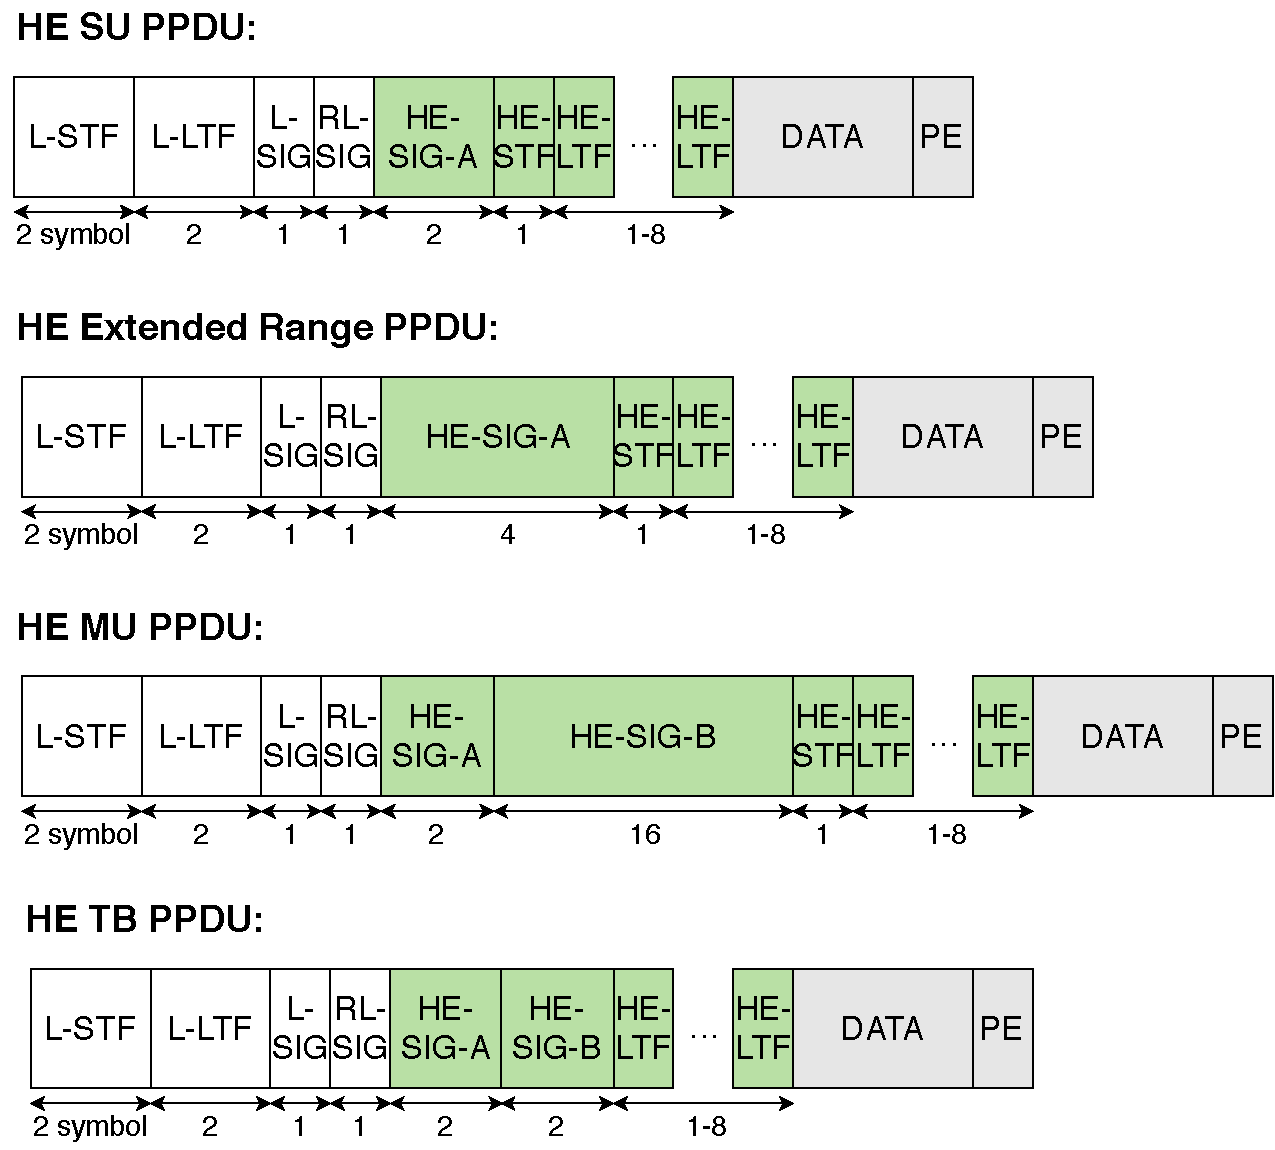
\epsfig{file=fig_25.pdf, width=.6\columnwidth}
	\caption{HE PPDU formats. New IEEE 802.11ax fields are highlighted in green.}
	\label{fig:appendix_1}
\end{figure}

Among the new fields, we highlight HE-SIG-A, which includes the following elements related to the SR operation:
\begin{itemize}
	\item BSS color: it is used as an identifier of the BSS (refer to Section \ref{section:bss_coloring}).
	\item Spatial Reuse: this field indicates whether the HE node supports the SR operation. If this is the case, the field also indicates the limit on the transmission power to be used during the SR opportunities that can potentially be detected. Notice that a single Spatial Reuse field (of length of 4 bits) is carried in HE SU/MU/ER PPDUs,  while HE TB PPDUs may include up to four Spatial Reuse fields. In particular, each field is meant for the SR operation in each allowed channel width (i.e., 20 MHz, 40 MHz, 80 MHz, and 160 MHz).
\end{itemize}

Besides supporting HE PPDU formats, HE STAs are required to be compatible with legacy formats. More information regarding HE PPDU formats can be found in \cite{rhode2017whitepaper}. 

% Other
\subsection{Management Fields for Spatial Reuse}
Some operations auxiliary to SR are enabled by control frames, which are Beacon, Probe Response, and (Re)Association Response frames. Beacons are used by APs to announce the presence of a BSS and to provide details of it. In particular, an AP, by means of Beacons, may request a STA to gather information regarding the environment: information of BSSs matching a particular BSSID and/or SSID, channel-specific report, or HE Operation element of neighboring HE APs. With this information, the AP can make decisions related to the SR operation. Regarding Probe Responses, they are meant to carry the information requested by devices scanning the area through Probe Requests. Finally, (Re)Association Response frames are sent by APs to which a STA attempts to associate.

The abovementioned kind of frames are important to the SR operation because they carry, among other fields, the following information:
\begin{itemize}
	\item \textbf{HE Capabilities:} it is used by HE STAs to announce support for certain HE capabilities.
	\item \textbf{HE Operation:} it defines the operation of HE STAs. For instance, it indicates whether BSS coloring is enabled or not.
	\item \textbf{BSS Color Change Announcement:} it is used by HE APs to indicate the utilization of a new BSS color so that the associated STAs and the surrounding devices can be aware of the change.
	\item \textbf{Spatial Reuse Parameter Set (SRPS) element:} this element provides the necessary information to carry out the OBSS/PD-based SR operation, which is defined in Section \ref{section:obss_pd_based}. The SRPS element is further defined in Appendix \ref{section:srps}.
\end{itemize}

\subsubsection{Spatial Reuse Parameter Set element}
\label{section:srps}
The format of the SRPS element is optionally present in Beacons, Probe Responses and (Re)Association responses. Figure 	\ref{fig:appendix_2} shows the SRPS element in detail.
% SR PARAMETER SET ELEMENT
\begin{figure}[ht!]
	\centering
	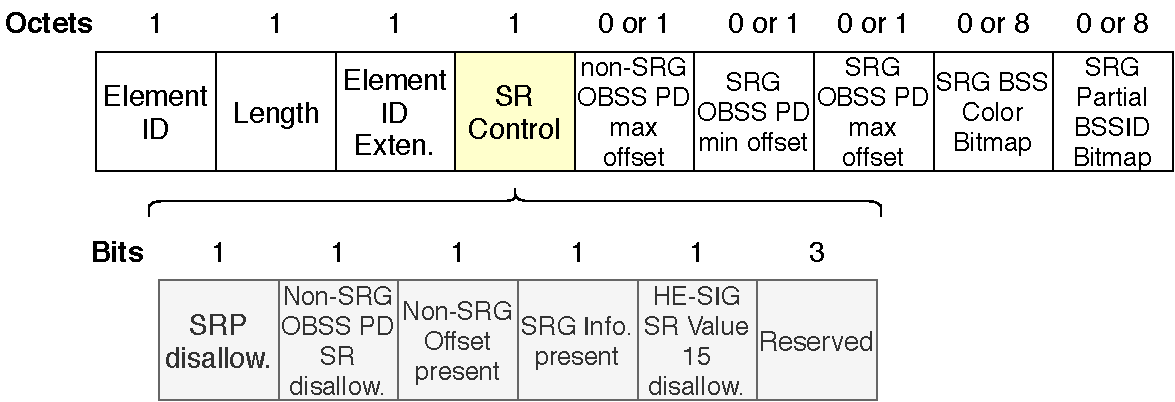
\epsfig{file=fig_26.pdf, width=.9\columnwidth}
	\caption{Spatial Reuse Parameter Set element.}
	\label{fig:appendix_2}
\end{figure}

Each item in the SRPS element is next described:
\begin{itemize}
	\item Element ID: set to 255.
	\item Length: not defined.
	\item Element ID extension: set to 39.
	\item SR Control field: contains the following parameters:
	\begin{itemize}
		\item PSR Disallowed: indicates whether PSR transmissions are allowed or not at non-AP STAs that are associated with the AP that transmitted this element.
		\item Non-SRG OBSS/PD SR Disallowed: indicates whether non-SRG OBSS/PD SR transmissions are allowed or not at non-AP STAs that are associated with the AP that transmitted this element.
		\item Non-SRG Offset Present: indicates whether the Non-SRG OBSS/PD Max Offset subfield is present in the element.
		\item SRG Information Present: indicates whether the SRG OBSS/PD Min Offset, SRG OBSS/PD Max Offset, SRG BSS Color Bitmap, and SRG Partial BSSID Bitmap subfields are present in the element.
		\item HE-SIG-A Spatial Reuse Value 15 disallow: indicates whether non-AP STAs that are associated with the AP that transmitted this element may set the TXVECTOR parameter SPATIAL\_REUSE to PSR\_AND\_NON-SRG-OBSS-PD\_PROHIBITED to avoid PSR transmissions.
	\end{itemize}
	\item Non-SRG OBSS/PD Max Offset: integer to generate the maximum Non-SRG OBSS/PD threshold.
	\item Non-SRG OBSS/PD Min Offset: integer to generate the minimum Non-SRG OBSS/PD threshold.
	\item SRG OBSS/PD Max Offset: integer to generate the maximum SRG OBSS/PD threshold.
	\item SRG BSS Color Bitmap: indicates which BSS Color values are used by the members of the SRG.
	\item SRG Partial BSSID Bitmap: indicates which partial BSSID values are used by members of the SRG.
\end{itemize}

\end{appendices}

\section*{Acknowledgment}
This  work  has  been  partially  supported  by  the  Spanish Ministry of Economy and Competitiveness under the Maria de Maeztu  Units  of  Excellence  Programme  (MDM-2015-0502), by PGC2018-099959-B-100 (MCIU/AEI/FEDER,UE), by the Catalan Government under SGR grant for research support (2017-SGR-11888), by SPOTS project (RTI2018-095438-A-I00) funded by the Spanish Ministry of Science, Innovation and Universities, and  by a Gift from the Cisco University Research Program (CG\#890107, Towards Deterministic Channel Access in High-Density WLANs) Fund, a corporate advised fund of Silicon Valley Community Foundation.

The authors would like to thank Dr. Malcolm Smith and Dr. Adrian Garcia for their thorough reviews and insightful comments.

\bibliographystyle{unsrt}
\bibliography{bib}


\end{document}
